%
% User guide for ExEfProb: Exact Effectus Probability
%
% Conventions
% ===========
%
% - Write \Python to refer to the language; similarly for \EfProb
%
% - Use British spelling in explanation, US for programming
%
% - within \index{...} use ~ instead of a space. In sub-index use a 
%   and two hyphens if the main work is repeated at the end, like in
%   \index{state!quantum~--}
%
% - Use marginpar instead of sidenote to describe a ``todo'' item
%
% - Use \cite{} instead of \citep{}, so that references appear in 
%   the margin
%
%
%
% Discussion points
% =================
%
% - importance of checking that something is a state/predicate
%   * associated: allow syntac 0.3*s + 0.7*t for states s,t
%
% - as_pred or aspred? What is done elsewhere in python
%
%
% Remarks
% =======
%%
%% - package Qcuircuit for drawing quantum circuit diagrams at:
%%   http://physics.unm.edu/CQuIC/Qcircuit/
%% - check Stochastic Matlab
%% - https://www.manning.com/books/practical-probabilistic-programming
%% - many models at (including GPA):
%%   http://forestdb.org/
%%
%% ToDo's
%% ======
%%

%% - Mermin Magic square via Pauli operators: 3x3 square, only 0,1,
%%   each row and the first two columns have parity zero, the third
%%   one has parity one ??  
%%
%%   Generalisations of these are getting atten
%
% Literature
% ==========
%
%  https://en.wikipedia.org/wiki/Quantum_cognition
%
\documentclass[leqno]{tufte-book} % Use the tufte-book class which in
                                  % turn uses the tufte-common class

\newif\ifignore % when set to true, additional text appears containing
                % further explanations or proofs (see \auxproof below)
%\ignoretrue 
\ignorefalse
\newcommand{\auxproof}[1]{
\ifignore\mbox{}\newline
\textbf{PROOF:} \dotfill\newline
{\it #1}\mbox{}\newline
\textbf{ENDPROOF}\dotfill
\fi}

\hypersetup{colorlinks} % Comment this line if you don't wish to have
                        % colored links

\usepackage{microtype} % Improves character and word spacing

\usepackage{lipsum} % Inserts dummy text

\usepackage{booktabs} % Better horizontal rules in tables

\usepackage{graphicx} % Needed to insert images into the document

\graphicspath{{graphics/}} % Sets the default location of pictures

\setkeys{Gin}{width=\linewidth,totalheight=\textheight,keepaspectratio} 
% Improves figure scaling

\usepackage{fancyvrb} % Allows customization of verbatim environments
\usepackage{qcircuit}
\usepackage{listings} 
\usepackage{fancybox,shadow}
%\usepackage{etex} % to get more space
\usepackage{amsmath}
%\usepackage{amssymb}
%\usepackage{amstext}
%\usepackage{mathtools}
%\usepackage{mathrsfs}
%\usepackage{stmaryrd}
%\usepackage{enumitem}
%\usepackage{cmll}
\usepackage{eurosym}
\usepackage{hyperref}
\usepackage{refcount}
\usepackage{url}
\usepackage{xspace} 
\usepackage{MnSymbol}
%\usepackage{nccmath}
%\usepackage{fancybox}
%\usepackage{xypic}
%\usepackage{xy}
%\xyoption{v2}
%\xyoption{curve}
%\xyoption{2cell}
%\UseTwocells
%\def\labelstyle{\textstyle}
%\def\twocellstyle{\textstyle}

\usepackage{xparse}
\usepackage{todonotes}
\presetkeys{todonotes}{size=\footnotesize,color=orange!30}{}
% For comments
\NewDocumentCommand\mycomment{om}{%
  \todo[color=blue!20]{%
  \IfNoValueF{#1}{\textbf{#1:} }#2}%
}

\input prooftree

\renewcommand{\arraystretch}{1.3}
\setlength{\arraycolsep}{2pt}



\setcounter{secnumdepth}{2} % number up-to subsections
\setcounter{tocdepth}{3}


\newtheorem{theorem}{Theorem}
\newtheorem{lemma}[theorem]{Lemma}
\newtheorem{proposition}[theorem]{Proposition}
\newtheorem{corollary}[theorem]{Corollary}
\newtheorem{definition}[theorem]{Definition}
\newtheorem{example}[theorem]{Example}
\newtheorem{examples}[theorem]{Examples}
\newtheorem{remark}[theorem]{Remark}
\newtheorem{question}[theorem]{Question}
\newtheorem{conjecture}[theorem]{Conjecture}


%
% Part of the stuff below can be removed.
%
\fvset{fontsize=\normalsize} % The font size of all verbatim text can
                             % be changed here

\newcommand{\hangp}[1]{\makebox[0pt][r]{(}#1\makebox[0pt][l]{)}} 
% New command to create parentheses around text in tables which take
% up no horizontal space - this improves column spacing

\newcommand{\hangstar}{\makebox[0pt][l]{*}} 
% New command to create asterisks in tables which take up no
% horizontal space - this improves column spacing

%\usepackage{xspace} 
% Used for printing a trailing space better than using a tilde (~)
% using the \xspace command

\newcommand{\monthyear}{\ifcase\month\or January\or February\or March\or April\or May\or June\or July\or August\or September\or October\or November\or December\fi\space\number\year} % A command to print the current month and year

\newcommand{\openepigraph}[2]{ % This block sets up a command for
                               % printing an epigraph with 2 arguments
                               % - the quote and the author
\begin{fullwidth}
\sffamily\large
\begin{doublespace}
\noindent\allcaps{#1}\\ % The quote
\noindent\allcaps{#2} % The author
\end{doublespace}
\end{fullwidth}
}

\newcommand{\blankpage}{\newpage\hbox{}\thispagestyle{empty}\newpage} 
% Command to insert a blank page

%\usepackage{units} % Used for printing standard units

\newcommand{\hlred}[1]{\textcolor{Maroon}{#1}} % Print text in maroon

\newcommand{\hangleft}[1]{\makebox[0pt][r]{#1}} 
% Used for printing commands in the index, moves the slash left so the
% command name aligns with the rest of the text in the index

\newcommand{\hairsp}{\hspace{1pt}} % Command to print a very short space

\newcommand{\ie}{\textit{i.\hairsp{}e.}\xspace} % Command to print i.e.

\newcommand{\eg}{\textit{e.\hairsp{}g.}\xspace} % Command to print e.g.
\newcommand{\etc}{\textit{etc.}\xspace} % Command to print e.g.

\newcommand{\na}{\quad--} % Used in tables for N/A cells

%\newcommand{\measure}[3]{#1/#2$\times$\unit[#3]{pc}} 
% Typesets the font size, leading, and measure in the form of:
% 10/12x26 pc.

\newcommand{\tuftebs}{\symbol{'134}} 
% Command to print a backslash in tt type in OT1/T1

\providecommand{\XeLaTeX}{X\lower.5ex\hbox{\kern-0.15em\reflectbox{E}}\kern-0.1em\LaTeX}

\newcommand{\tXeLaTeX}{\XeLaTeX\index{XeLaTeX@\protect\XeLaTeX}} 
% Command to print the XeLaTeX logo while simultaneously adding the
% position to the index

\newcommand{\doccmdnoindex}[2][]{\texttt{\tuftebs#2}} 
% Command to print a command in texttt with a backslash of tt type
% without inserting the command into the index

\newcommand{\doccmddef}[2][]{\hlred{\texttt{\tuftebs#2}}\label{cmd:#2}\ifthenelse{\isempty{#1}} % Command to define a command in red and add it to the index
{ % If no package is specified, add the command to the index
\index{#2 command@\protect\hangleft{\texttt{\tuftebs}}\texttt{#2}}% Command name
}
{ % If a package is also specified as a second argument, add the command and package to the index
\index{#2 command@\protect\hangleft{\texttt{\tuftebs}}\texttt{#2} (\texttt{#1} package)}% Command name
\index{#1 package@\texttt{#1} package}\index{packages!#1@\texttt{#1}}% Package name
}}

\newcommand{\doccmd}[2][]{% Command to define a command and add it to the index
\texttt{\tuftebs#2}%
\ifthenelse{\isempty{#1}}% If no package is specified, add the command to the index
{%
\index{#2 command@\protect\hangleft{\texttt{\tuftebs}}\texttt{#2}}% Command name
}
{%
\index{#2 command@\protect\hangleft{\texttt{\tuftebs}}\texttt{#2} (\texttt{#1} package)}% Command name
\index{#1 package@\texttt{#1} package}\index{packages!#1@\texttt{#1}}% Package name
}}

% A bunch of new commands to print commands, arguments, environments,
% classes, etc within the text using the correct formatting
\newcommand{\docopt}[1]{\ensuremath{\langle}\textrm{\textit{#1}}\ensuremath{\rangle}}

\newcommand{\docarg}[1]{\textrm{\textit{#1}}}

\newenvironment{docspec}{\begin{quotation}\ttfamily\parskip0pt\parindent0pt\ignorespaces}{\end{quotation}}

\newcommand{\docenv}[1]{\texttt{#1}\index{#1 environment@\texttt{#1} environment}\index{environments!#1@\texttt{#1}}}

\newcommand{\docenvdef}[1]{\hlred{\texttt{#1}}\label{env:#1}\index{#1 environment@\texttt{#1} environment}\index{environments!#1@\texttt{#1}}}

\newcommand{\docpkg}[1]{\texttt{#1}\index{#1 package@\texttt{#1} package}\index{packages!#1@\texttt{#1}}}

\newcommand{\doccls}[1]{\texttt{#1}}

\newcommand{\docclsopt}[1]{\texttt{#1}\index{#1 class option@\texttt{#1} class option}\index{class options!#1@\texttt{#1}}}

\newcommand{\docclsoptdef}[1]{\hlred{\texttt{#1}}\label{clsopt:#1}\index{#1 class option@\texttt{#1} class option}\index{class options!#1@\texttt{#1}}}

\newcommand{\docmsg}[2]{\bigskip\begin{fullwidth}\noindent\ttfamily#1\end{fullwidth}\medskip\par\noindent#2}

\newcommand{\docfilehook}[2]{\texttt{#1}\index{file hooks!#2}\index{#1@\texttt{#1}}}

\newcommand{\doccounter}[1]{\texttt{#1}\index{#1 counter@\texttt{#1} counter}}

\usepackage{makeidx} % Used to generate the index
\makeindex % Generate the index which is printed at the end of the document

% This block contains a number of shortcuts used throughout the book

%
% Names
%
\newcommand{\EfProb}{\textit{EfProb}\xspace}
\newcommand{\Python}{\textrm{Python}\xspace}

%
% Abbreviations
%
\newcommand{\CN}{\mathbb{C}}     % complex numbers
\newcommand{\RN}{\mathbb{R}}     % real numbers
\newcommand{\RNpos}{\RN_{\geq 0}}  % positive real numbers
\newcommand{\NN}{\mathbb{N}}     % natural numbers
\newcommand{\Mat}{\mathsf{M}}
\newcommand{\tr}{\mathsf{tr}}
\newcommand{\gp}{\mathsf{gp}}
\newcommand{\extr}{\mathsf{extr}}
\newcommand{\lb}{\mathsf{lb}}
\newcommand{\ub}{\mathsf{ub}}
\newcommand{\intd}{{\kern.2em}\mathrm{d}{\kern.03em}}
\newcommand{\andthen}{\mathrel{\&}}
\newcommand{\truth}{\mathsf{truth}}
\newcommand{\falsity}{\mathsf{falsity}}
\newcommand{\scalar}{\mathrel{*}}

%
% Logic
%
\newcommand{\all}[2]{\forall{#1}.\,#2}
\newcommand{\allin}[3]{\forall{#1\in#2}.\,#3}
\newcommand{\ex}[2]{\exists{#1}.\,#2}
\newcommand{\exin}[3]{\exists{#1\in#2}.\,#3}
\newcommand{\lam}[2]{\lambda#1.\,#2}
\newcommand{\lamin}[3]{\lambda#1\in#2.\,#3}
\newcommand{\tuple}[1]{\langle#1\rangle}
\newcommand{\one}{\ensuremath{\mathbf{1}}}
\newcommand{\zero}{\ensuremath{\mathbf{0}}}

%
% Probability
%
\newcommand{\ket}[1]{\ensuremath{|#1\rangle}}
\newcommand{\bigket}[1]{\ensuremath{\big|#1\big\rangle}}
\newcommand{\bra}[1]{\langle\,#1\,|}
\newcommand{\bigbra}[1]{\ensuremath{\big\langle#1\big|}}
\newcommand{\ortho}{\mathop{\sim}}
\newcommand{\tensor}{\mathrel{@}}
\newcommand{\indic}[1]{\mathbf{1}_{#1}}
\newcommand{\Prob}[1]{\mathrm{Pr}\left({#1}\right)}



%
% Category theory
%
\newcommand{\Dst}{\mathcal{D}}
\newcommand{\Mlt}{\mathcal{M}}
\newcommand{\Giry}{\mathcal{G}}


%
% Miscellenuous
%
\newcommand{\Qdiscard}{\rule{0.2em}{1em}}
\newcommand{\idmap}[1][]{\ensuremath{\mathrm{id}_{#1}}}
\newcommand{\after}{\mathrel{\circ}}


\newcommand{\cgr}[2][scale=0.45]{\raisebox{0.1em}{\begingroup
\setbox0=\hbox{\includegraphics[#1]{#2}}%0
\parbox{\wd0}{\box0}\endgroup}}


% Python style for highlighting
% Default fixed font does not support bold face
\DeclareFixedFont{\ttb}{T1}{txtt}{bx}{n}{12} % for bold
\DeclareFixedFont{\ttm}{T1}{txtt}{m}{n}{12}  % for normal
% Custom colors
\usepackage{color}
\definecolor{deepblue}{rgb}{0,0,0.5}
\definecolor{deepred}{rgb}{0.6,0,0}
\definecolor{deepgreen}{rgb}{0,0.5,0}

\newcommand\pythonstyle{\lstset{
language=Python,
basicstyle=\ttm,
otherkeywords={self,>>>},             % Add keywords here
keywordstyle=\ttb\small\color{deepblue},
emph={@,+\%%
% fix needed for highlighting operators
literate={.+}{{{\color{red}.+}}}2 {.**}{{{\color{red}.\**{}}}}2 {*}{{{\color{red}*}}}1
},          % Custom highlighting
emphstyle=\ttb\small\color{deepred},    % Custom highlighting style
stringstyle=\small\color{deepgreen},
frame=tb,                         % Any extra options here
showstringspaces=false            % 
}}
\lstnewenvironment{python}[1][] % Python environment
{
%\begin{fullwidth}
%\begin{minipage}{\textwidth}
\pythonstyle
\lstset{basicstyle=\normalfont\ttfamily\small#1}
%\end{fullwidth}
%\end{minipage}
}
{}
\newcommand\pythonexternal[2][]{{ % Python for external files
\pythonstyle
\lstinputlisting[#1]{#2}}}
\newcommand\pythoninline[1]{\pythonstyle\lstinline[basicstyle=\normalfont\ttfamily\small]{#1}} % Python for inline

%----------------------------------------------------------------------------------------
%	BOOK META-INFORMATION
%----------------------------------------------------------------------------------------

\title{EfProb User Manual
%\thanks{Thanks to Edward R.~Tufte for his inspiration.}
} 

\author[Jacobs \& Cho]{Bart Jacobs and Kenta Cho} % Author

%\publisher{Publisher of This Book} % Publisher

%----------------------------------------------------------------------------------------

\begin{document}

\frontmatter

%----------------------------------------------------------------------------------------
%	EPIGRAPH
%----------------------------------------------------------------------------------------

%% \thispagestyle{empty}
%% \openepigraph{The public is more familiar with bad design than good design. It is, in effect, conditioned to prefer bad design, because that is what it lives with. The new becomes threatening, the old reassuring.}{Paul Rand, {\itshape Design, Form, and Chaos}}
%% \vfill
%% \openepigraph{A designer knows that he has achieved perfection not when there is nothing left to add, but when there is nothing left to take away.}{Antoine de Saint-Exup\'{e}ry}
%% \vfill
%% \openepigraph{\ldots the designer of a new system must not only be the implementor and the first large-scale user; the designer should also write the first user manual\ldots If I had not participated fully in all these activities, literally hundreds of improvements would never have been made, because I would never have thought of them or perceived why they were important.}{Donald E. Knuth}

%----------------------------------------------------------------------------------------

\maketitle 

%% %----------------------------------------------------------------------------------------
%% %	COPYRIGHT PAGE
%% %----------------------------------------------------------------------------------------

%% \newpage
%% \begin{fullwidth}
%% ~\vfill
%% \thispagestyle{empty}
%% \setlength{\parindent}{0pt}
%% \setlength{\parskip}{\baselineskip}
%% Copyright \copyright\ \the\year\ \thanklessauthor

%% \par\smallcaps{Published by \thanklesspublisher}

%% \par\smallcaps{tufte-latex.googlecode.com}

%% \par Licensed under the Apache License, Version 2.0 (the ``License''); you may not use this file except in compliance with the License. You may obtain a copy of the License at \url{http://www.apache.org/licenses/LICENSE-2.0}. Unless required by applicable law or agreed to in writing, software distributed under the License is distributed on an \smallcaps{``AS IS'' BASIS, WITHOUT WARRANTIES OR CONDITIONS OF ANY KIND}, either express or implied. See the License for the specific language governing permissions and limitations under the License.\index{license}

%% \par\textit{First printing, \monthyear}
%% \end{fullwidth}

\tableofcontents 
%\listoffigures 
%\listoftables 

%% %----------------------------------------------------------------------------------------
%% %	DEDICATION PAGE
%% %----------------------------------------------------------------------------------------

%% \cleardoublepage
%% ~\vfill
%% \begin{doublespace}
%% \noindent\fontsize{18}{22}\selectfont\itshape
%% \nohyphenation
%% Dedicated to those who appreciate \LaTeX{} and the work of \mbox{Edward R.~Tufte} and \mbox{Donald E.~Knuth}.
%% \end{doublespace}
%% \vfill
%% \vfill



\cleardoublepage
\chapter{Introduction} 

This text gives a hands-on introduction to the \EfProb library.  The
latter is an embbeded language in \Python, for probability.  The
`\textit{Ef}' in \EfProb stands for `Effectus', and `\textit{Prob}
stand for `Probability'. An effectus\index{effectus} is an abstract
(categorical) model that captures the essentials of discrete,
continuous and quantum probability and
logic\cite{Jacobs15,ChoJWW15}. The \EfProb library is based on this
categorical model, providing a uniform approach to discrete,
continuous, and quantum probability. However, in order to be able to
use and understand the basic of the \EfProb library it is not required
to understand the underlying categorical semantics.

The \EfProb library makes it easy to model various problems in
probability theory and to compute outcomes: probabilities of events
and of predicates can be computed, product and conditional states can
be formed, expectations and variances can be calculated, \etc These
computations can be done for \eg~Bayesian networks, hidden Markov
models, stochastic kernels, and quantum protocols.

The library consists of two \Python files:
\begin{enumerate}
\item \pythoninline{efprob\_dc.py}, for discrete and continuous
  probability, in combined form, discused in Chapters~\ref{ch:dp}
  and~\ref{ch:cp};

\item \pythoninline{efprob\_qu.py}, for quantum probability, described in
  Chapter~\ref{ch:qp}.
\end{enumerate}

\noindent There is some overlap in the explanations in the three
chapters. This is intentional, so that these chapters can be read
largely independently.  The reader is encouraged to load these files
before studying the relevant chapters, and to try out the examples and
make variations on them while progressing through the text.

In the text below many examples are shown using \Python in interactive
mode, from the command line, as in:
\begin{python}
>>> from efprob_dc import *
>>> s = flip(0.2)
>>> s
0.2|True> + 0.8|False>
\end{python}

\noindent The lines starting with \pythoninline{>>>} describe user
input, and the other lines describe the output given by the system.
The first line imports the relevant library. It will be omitted in the
sequel. 

All the examples used in this manual are also collected in three
separate files, with minimal explanations. These files have
self-explanatory names:
\begin{itemize}
\item \pythoninline{discrete-illustrations.py}
\item \pythoninline{continuous-illustrations.py}
\item \pythoninline{quantum-illustrations.py}
\end{itemize}

\noindent These files can be excuted, modified, and studied more
closely.

The basics of the \EfProb library exist and are reasonably stable.
This basis is already being used in several research papers. This
usage is the reason for publicly releasing the library at this early
stage, so that results can be reconstructed and checked by
others. Further research on extensions and adaptations of the basic
library are still going on. Therefore new versions will appear from
time to time.

For the same reason, this manual is still evolving, and is incomplete
as it stands. Still we hope that it is useful, because it already
explains many basic aspects of the library and contains several
examples of how it can be used.

We conclude this introduction with several loosely related remarks
about the \EfProb library.
\begin{itemize}
\item The focus of the development of the library is on providing a
  new language and logic for probability, based on states and
  predicates. The library is not meant for large scale computation,
  for instance like in data analytics. In our development of the
  library we prefer semantical clarity to execution speed. Also, the
  \EfProb library does not come with any guarantees with respect to
  the correctness of the outcomes, see also the discussion about
  precision and side-conditions below.

\item We envision that the library could be useful in \emph{teaching}
  the basics of probability theory from a unified perspective. The
  \EfProb library is especially useful in quickly calculating
  probabilities, and experimenting with various formulations.

\item At the same time the library could be useful in scientific
  \emph{research} as well, in order to quickly model new examples and
  compute outcomes. We request that usage of the \EfProb library, if
  any, is mentioned in the acknowledgements of research papers.

\item The \EfProb library requires \Python, version $\geq$ 3.5.
  \EfProb heavily relies on existing libraries in \Python, in
  particular \pythoninline{math} and \pythoninline{numpy} (used as
  \pythoninline{np}) for linear algebra and matrices.

\item It is important to keep in mind that the main functionality of
  the library is \emph{computing} numerical outcomes, and not, for
  instance, logical reasoning. Often, these numerical outcomes are
  approximations, arising from the inherent limitations of using a
  computer for real number arithmetic. Sometimes we do use random
  states and/or random predicates to \emph{test} certain
  properties. But these numerical tests should never be taken as a
  logical \emph{proof}.

\item Despite the fact that numerical approximations are used in the
  EfProb calculations, the underlying semantics is \emph{exact}, and
  the library computes probabilities using the standard mathematical
  formulas, including, for instance, integration. This is in contrast
  to languages based on sampling, such as BLOG\cite{MilchMRSOK07} and
  Church\cite{GoodmanMRBT08}.

\item Many mathematical structures used in probability theory are
  required to satisfy certain properties. For instance: the
  probabilities occurring in a distribution must add up to one; or:
  the integral over the domain of definition of a probability density
  function (pdf) must be one; or: a quantum state is a matrix that
  must be positive and have a trace that is equal to one.

A fundamental question that exists in the current setting is: should
such properties be checked by \EfProb or should it be left as a
responsability of the user that these properties are satisfied --- for
instance when defining distributions / pdf's / quantum states?

Here it is relevant that in the presence of computational
approximations equations --- such as: a trace equals one --- can never
be checked reliable. In the continuous case the problem is more
serious, since it must be checked that a certain property
(\eg~positivity of a function) holds for infinitely many points, and
it's not effectively possible to do so. Hence, necessarily, the
responsability for side-conditions lies with the user.

That being said, the \EfProb does perform a few basic checks,
sometimes using margins of error. In our experience, these checks can
be useful to detect and prevent mistakes. Some check functions only
print warnings, explaining the margins, when side-conditions fail. The
checking of side-conditions is thus handled pragmatically. It is one
of the least stable parts of the library.

\item Because side-conditions are not checked systematically, the
  \EfProb language is unsafe. What we have is the familiar tension
  between expressive embedded languages and denotationally-sound
  type-safe languages.
% Quoted from Qwire paper.

But again, the \EfProb library does perform some basic checks. For
instance, states, predicates and channels use `domains' as types, as
will be explained below. It is checked that types match, for instance
when the validity of a predicate in a state is computed, or when
state/predicate transformation is applied. In case of a non-match, an
exception is thrown.
\end{itemize}


%----------------------------------------------------------------------------------------

\mainmatter

%----------------------------------------------------------------------------------------
%	CHAPTER 1
%----------------------------------------------------------------------------------------

\chapter{Discrete Probability}\label{ch:dp}

A \emph{discrete finite probability distribution},\index{distribution}
or simply a \emph{distribution} for short, is a weighted combination
of `things', where the weights are numbers from the unit interval
$[0,1]$ that add up to one. Such a weighted sum is also called a
\emph{convex combination}.\index{convex!combination} Here is an
example, using the RGB colour model.  This model describes each colour
as an additive combination of the primary colours red (R), green (G)
and blue (B). A particular colour can then be described as a convex
combination:
$$0.3\ket{R} + 0.2\ket{G} + 0.5\ket{B}.$$

\noindent This formal sum describes a particular weighted combination
of red, green, and blue. The `ket' notation $\ket{-}$ is borrowed from
the quantum world. It has no mathematical meaning, but is convenient
to separate the weights in the unit interval $[0,1]$ from the `things'
that are weighed. A graphical representation (`plot') of the above
convex combination can be seen in the
margin.\marginnote[-5\baselineskip]{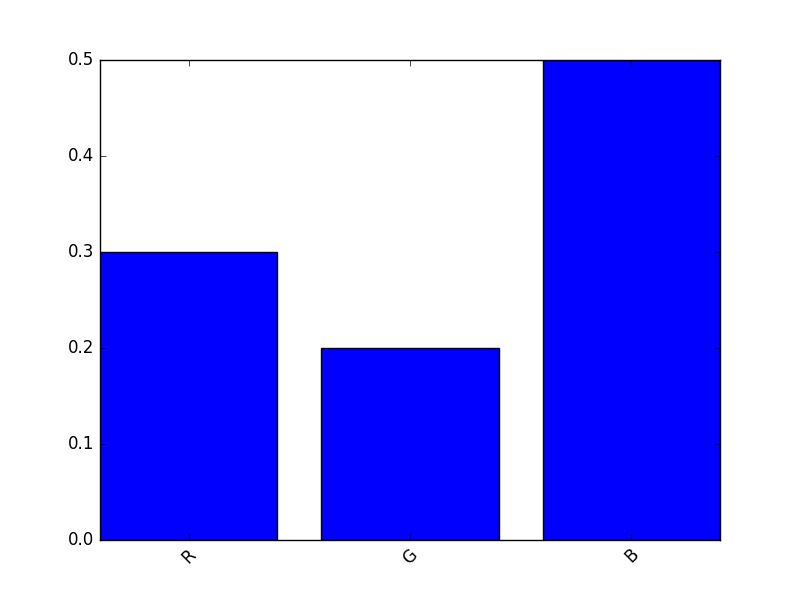
\includegraphics{Pictures/RGB.png}}

This chapter describes how to form such distributions, and how to
manipulate them via various other structures, like predicate, channels
and random variables. The same approach will be used for continuous
probability and also for quantum probability, so that the similarities
(and also some dissimilarities) between the three forms of probability
become clear. In order to emphasise this similarity, we will use
uniform terminology. Therefore, we often call a (discrete finite
probability) distribution a \emph{state}.


\section{States}\label{sec:dstate}

In our embedded language \EfProb within \Python one can define a
state for a fair (balanced) coin as:
\begin{python}
>>> fflip = State([0.5, 0.5], [True, False])
>>> fflip
0.5|True> + 0.5|False>
\end{python}

\noindent We see that the `things' that we weigh in this distribution
are in the second list argument of the class constructor
\pythoninline{State}. The set of these `things' is what we call the
\emph{domain} of the distribution. The elements of the domain of a
distribution are printed using the ket-notation $\ket{-}$, as
explained in the beginning of this
chapter. Subsection~\ref{subsec:dplot} below describes how
distributions can be plotted.

We can also define use another domain, as in:
\begin{python}
>>> fflipHT = State([0.5, 0.5], ['H', 'T'])
>>> fflipHT
0.5|H> + 0.5|T>
\end{python}

\noindent In principle, anything is allowed as domain element, as long
as it is already known to \Python at the moment that the state is
defined.\sidenote{One can define one's own domain elements in \Python,
  but this should be done before the definition of the state that uses
  these domain elements.}

\EfProb is an embedded language within \Python. This means that we
can define \Python itself to define a parametrised coin as:
\begin{python}
>>> def flip(r):
...     return State([r, 1-r], [True,False])
>>> flip(0.2)
0.2|True> + 0.8|False>
\end{python}

\noindent This \pythonstyle{flip} function is actually predefined in
\EfProb. 

In a similar way we can now define a fair dice as:\marginnote{The
  \EfProb library does not check or enforce that the probabilities in
  user-defined states add up to one. As explained in the introduction,
  the main reason is that such checks have limited value because of
  small precision errors in calculations in \Python. In addition, it
  gives some more flexibility, for instance to use
  \emph{subdistribution}, where the sum of probabilities is below
  one. The disadvantage of not having these checks is that
  non-probabilistic and even false results can be obtained.}
\begin{python}
>>> fdice = State([1/6,1/6,1/6,1/6,1/6,1/6], [1,2,3,4,5,6])
>>> fdice
0.167|1> + 0.167|2> + 0.167|3> + 0.167|4> + 0.167|5> + 0.167|6>
\end{python}

\noindent The probabilities are pretty-printed with only three
decimals. This can be adjusted in the library itself.

There is a predefined function for uniform distributions,
for which we only have to give the domain. Hence it is easier to
define:
\begin{python}
>>> fdice = uniform_state([1,2,3,4,5,6])
>>> fdice
0.167|1> + 0.167|2> + 0.167|3> + 0.167|4> + 0.167|5> + 0.167|6>
\end{python}

\noindent If you like, you can also use a sequence of points as
domain:
\begin{python}
>>> fdice = uniform_state(['*','**','***','****','*****','******'])
>>> fdice
0.167|*> + 0.167|**> + 0.167|***> + 0.167|****> + 0.167|*****> + 0.167|******>
\end{python}

\noindent There is also a function that produces a singleton state
$1\ket{x}$ with domain $D$ (which must contain $x$), namely
\pythoninline{point_state(x, D)}, see for instance:
\begin{python}
>>> point_state(True, [True,False])
1|True> + 0|False>
>>> point_state(3, [1,2,3,4,5,6])
0|1> + 0|2> + 1|3> + 0|4> + 0|5> + 0|6>
\end{python}

\noindent When you are happy with natural numbers as domain you
can use \Python's built-in function \pythoninline{range}.
For an arbitrary number $n$,
\pythoninline{range(n)} is the sequence
of $0, 1, 2, \dotsc, n-1$ and can be used as domain:
\begin{python}
>>> uniform_state(range(5))
0.2|0> + 0.2|1> + 0.2|2> + 0.2|3> + 0.2|4>
>>> point_state(2, range(4))
0|0> + 0|1> + 1|2> + 0|3>
\end{python}

\noindent The simplest possible distribution $1\ket{0}$ with domain
$\{0\}$ can be produced as \pythoninline{point_state(0,range(1))} or
also as \pythoninline{uniform_state(range(1))}.

For testing purposes it is useful to have a random discrete
probability. It works as described
below, internally using \Python's random number generator. Each time
it gives a different answer.
\begin{python}
>>> random_state(range(5))
0.133|0> + 0.273|1> + 0.175|2> + 0.119|3> + 0.3|4>
>>> random_state(range(5))
0.252|0> + 0.25|1> + 0.452|2> + 0.035|3> + 0.0103|4>
\end{python}



\begin{remark}
\label{rem:poisson}
As sketched above, several basic \emph{finite} discrete distributions
can be represented in \EfProb. But what about \emph{infinite}
discrete distributions? The most prominent example is the
\emph{Poisson} distribution, with the natural numbers $\NN$ as domain,
given by the formal sum:
$$\sum_{k\in\NN}\, \frac{\lambda^{k} \cdot e^{-\lambda}}{k!}\bigket{k}$$

\noindent where $\lambda \geq 0$ is the `mean' or `rate' parameter.

The representation of the Poisson distribution/state in \EfProb
involves restriction to a certain upper bound $\ub\in\NN$, making the
above distribution finite. But since the weights then no longer add up
to one, we compensate in an appropriate way. This representation is
thus an approximation of the `real' Poisson distribution, where the
user can choose the upper bound sufficiently high for the required
level of precision.

The implementation of this restricted Poisson distribution looks as
follows.
\begin{python}
def poisson(lam, ub):
    probabilities = [(lam ** k) * (e ** -lam) / factorial(k) 
                     for k in range(ub)]
    s = sum(probabilities)
    return State([p/s for p in probabilities], range(ub))
\end{python}

\noindent With mean $3$ and upperbound $20$ we see that the last
probability is already really small:
\begin{python}
>>> poisson(3,20)
0.0498|0> + 0.149|1> + 0.224|2> + 0.224|3> + ... + 3.01e-09|18> + 4.76e-10|19>
\end{python}
\end{remark}


\subsection{Operations on states}\label{subsec:dstate:operations}

The three standard operations on states are: product, convex sum, and
marginal. We discuss them one by one below.

\paragraph{Product states}
A `joint' or `product'
distribution/state\index{product!of~discrete~states}\index{state!discrete~product~--}
can be formed via the product operator \pythoninline{@}. For instance,
the product of a coin with bias \pythoninline{0.2} and a coin with
bias \pythoninline{0.7} is written as:
\begin{python}
>>> flip(0.2)
0.2|True> + 0.8|False>
>>> flip(0.7)
0.7|True> + 0.3|False>
>>> flip(0.2) @ flip(0.7)
0.14|True,True> + 0.06|True,False> + 0.56|False,True> + 0.24|False,False>
\end{python}

\noindent We see that the product distribution contains all possible
pairs of domain elements, with multiplied probabilities. Of course,
the sum of the weights is still one.

It is is not necessary that the two states that are combined in a
product have the same length or domain:
\begin{python}
>>> flip(0.2) @ uniform_state(range(4))
0.05|True,0> + 0.05|True,1> + 0.05|True,2> + 0.05|True,3> + 
   0.2|False,0> + 0.2|False,1> + 0.2|False,2> + 0.2|False,3>
\end{python}

\noindent Multiple products are also possible:
\begin{python}
>>> flip(0.2) @ uniform_state(range(4)) @ flip(0.8)
0.04|True,0,True> + 0.01|True,0,False> + 0.04|True,1,True> + 0.01|True,1,False> + 
   0.04|True,2,True> + 0.01|True,2,False> + 0.04|True,3,True> + 
   0.01|True,3,False> + 0.16|False,0,True> + 0.04|False,0,False> + 
   0.16|False,1,True> + 0.04|False,1,False> + 0.16|False,2,True> + 
   0.04|False,2,False> + 0.16|False,3,True> + 0.04|False,3,False>
\end{python}

\noindent Since the domain of a product state is the cartesian product
of the domains of the component states, such products states grow
quickly in size. If we have $k$ states $s_{1}, s_{2}, \ldots, s_{k}$,
where each state $s_i$ has domain size $n_{i}$, then the product state
$s_{1} \tensor s_{2} \tensor \cdots \tensor s_{k}$ has size $n_{1}
\cdot n_{2} \cdot \ldots \cdot n_{k}$.\sidenote{The parallel product
  operator \pythoninline{@} is `strictly' associative, so that
  \pythoninline{(s1 @ s2) @ s3} and \pythoninline{s1 @ (s2 @ s3)} are
  the same states.}

One can use \Python's power operator \pythoninline{**} to
get multiple products of a state with itself:
\begin{python}
>>> flip(0.2) ** 3
0.008|True,True,True> + 0.032|True,True,False> + 0.032|True,False,True> + 
   0.128|True,False,False> + 0.032|False,True,True> + 0.128|False,True,False> + 
   0.128|False,False,True> + 0.512|False,False,False>
\end{python}

\noindent This is the same as \pythoninline{flip(0.2) @ flip(0.2) @
  flip(0.2)}.


\paragraph{Convex sums of states} Discrete states are formal convex
sums over their domains. But there is an additional form of convex
sum,\index{convex!sum~of~discrete~states} namely of states
themselves. For instance in:
\begin{python}
>>> convex_state_sum((0.2,flip(0.3)), (0.5,flip(0.8)), (0.3,flip(1)))
0.76|True> + 0.24|False>
\end{python}

\noindent In such a convex sum of states it is required that the
weights (here: \pythoninline{0.2}, \pythoninline{0.5} and
\pythoninline{0.3}) add up to one and that all the states have the
same domain.



\paragraph{Marginalisation of joint states}

The product operation \pythoninline{@} \emph{constructs} a new, joint
state from `component' states. Marginalisation \emph{destructs} a
joint state. When applied to a state built with \pythoninline{@},
marginalisation returns the original components. In order to give a
bit more generality to a demonstration like the one below, we use
randomly generated states.
\begin{python}
>>> s = random_state(range(3))
>>> t = random_state(range(2))
>>> s
0.255|0> + 0.465|1> + 0.28|2>
>>> t
0.507|0> + 0.493|1>
>>> s @ t
0.13|0,0> + 0.126|0,1> + 0.236|1,0> + 0.229|1,1> + 0.142|2,0> + 0.138|2,1>
>>> (s @ t) % [1,0]
0.255|0> + 0.465|1> + 0.28|2>
>>> (s @ t) % [0,1]
0.507|0> + 0.493|1>
\end{python}

\noindent We use the post-fix operation \pythoninline{\% [1,0]} for
the \emph{first} marginal, and \pythoninline{\% [0,1]} for the
\emph{second} marginal. On a state built up from $n$ components one
can use `selectors' given by a list of $n$ \pythoninline{0}'s and
\pythoninline{1}'s. A `\pythoninline{1}' at position $i$ means: keep
this $i$-th component; a `\pythoninline{0}' at position $i$ says:
delete this $i$-th component. For instance we remove the
really big state and keep the two smaller ones in:
\begin{python}
>>> (random_state(range(100)) @ flip(0.5) @ uniform_state(range(2))) % [0,1,1]
0.25|True,0> + 0.25|True,1> + 0.25|False,0> + 0.25|False,1>
\end{python}

\noindent Marginalisation involves summation over all probabilities
that are projected out, \ie~that are discarded in a certain dimension,
as indicated by a \pythoninline{0} in a marginalisation selector
\pythoninline{\% [...]}. 

In general, a joint state \pythoninline{s} is called
\emph{independent} or \emph{non-entwined} if it is the product of its
marginals, that is, if it is equal to \pythoninline{(s \% [1,0]) @ (s
  \% [0,1])}. If the state \pythoninline{s} is defined as product
\pythoninline{s1 @ s2}, then it is always non-entwined. We shall see
an illustration of an entwined state (via conditioning) in
Example~\ref{ex:entwinednessviaconditioning}.

We add the following general observation about entwinedness of joint states.
\begin{equation}
\label{eqn:entwined}
\begin{array}{rcl}
\begin{array}{c}
r_{1}\ket{0,0} + r_{2}\ket{0,1} + r_{3}\ket{1,0} + r_{4}\ket{1,1}
\\[-.4em]
\mbox{is non-entwined}
\end{array}
& \quad\mbox{iff}\quad &
r_{1}\cdot r_{4} = r_{2}\cdot r_{3}
\end{array}
\end{equation}



\subsection{Plotting states}\label{subsec:dplot}

So far we have described states as finite formal convex sums
$r_{1}\ket{x_1} + \cdots + r_{n}\ket{x_n}$. The \EfProb library also
supports, to some extend, plotting states, as bar charts. The command
below generates the picture in the
margin.\marginnote[-3\baselineskip]{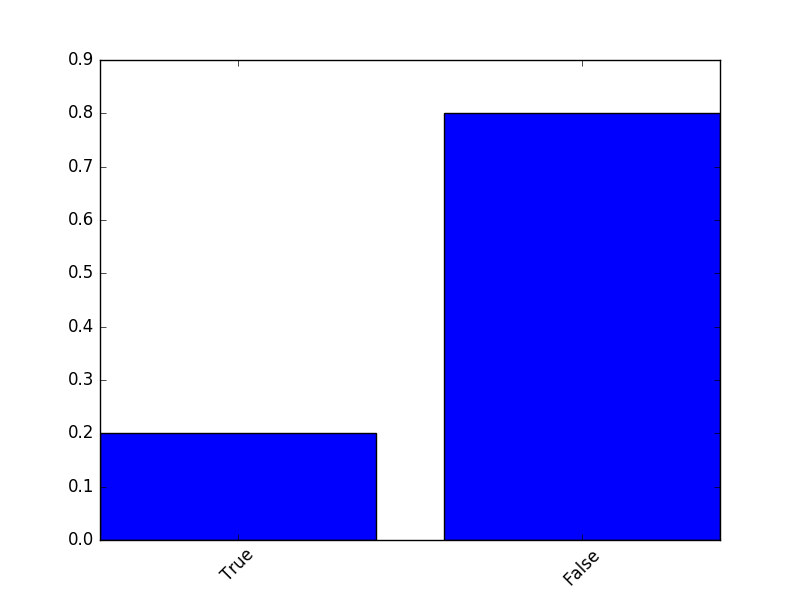
\includegraphics{Pictures/flip_02.png}}
\begin{python}
>>> flip(0.2).plot()
\end{python}

\noindent The probability of each element of the domain is indicated
by the height of the corresponding bar. This works for domains of a
`reasonable' size. For instance, the plot of the the state
\pythoninline{poisson(7,20)} gives the picture below.
\begin{center}
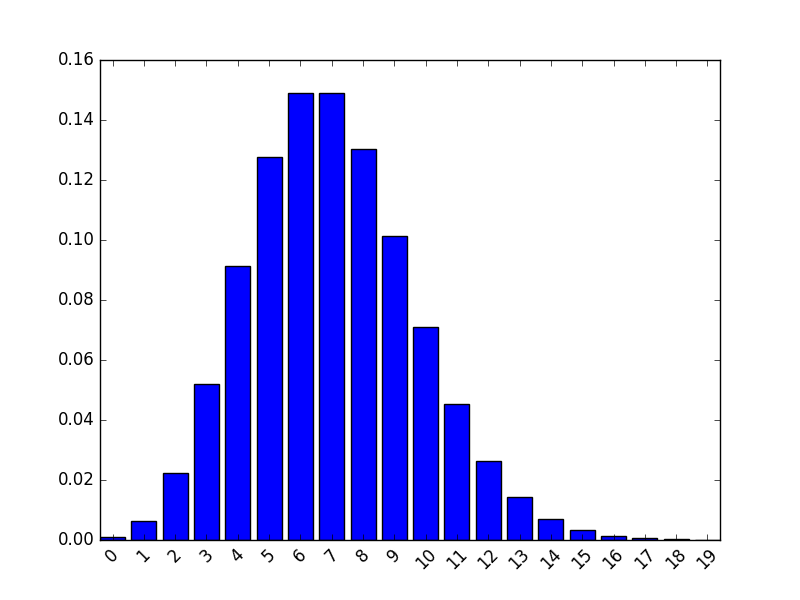
\includegraphics[width=!,totalheight=!,scale=0.5]{Pictures/poisson_7_20.png}
\end{center}

\noindent This is still quite readable. But when we move to a domain
of 50 elements the plot becomes quite dense and the individual domain
elements are hard to distinguish. The example below describes an
instance of \pythoninline{random\_disc\_state(50)}.
\begin{center}
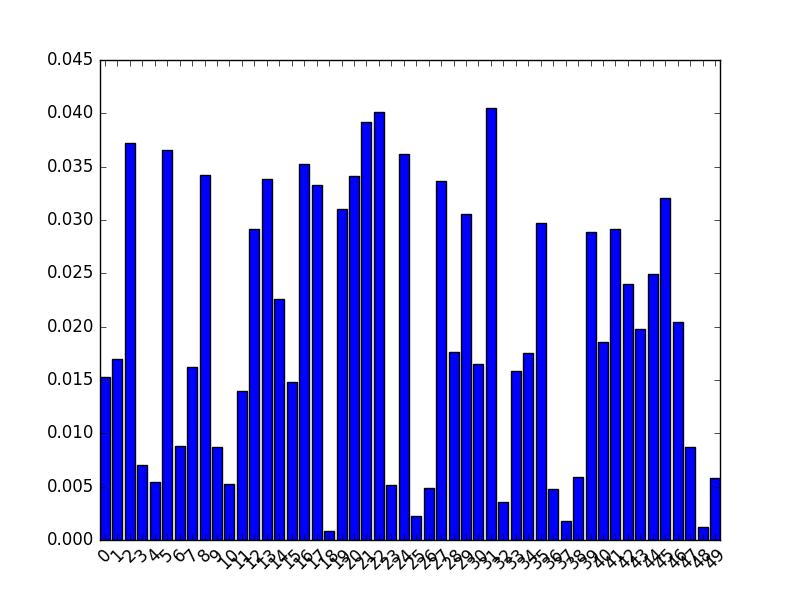
\includegraphics[width=!,totalheight=!,scale=0.5]{Pictures/random_disc_50.png}
\end{center}

A 2-dimensional product/joint state can also be plotted. In addition,
one can plot a `slice' of a product state, as shown below.
\begin{python}
>>> s = State([0.1,0.5,0.25,0.15], range(4))
>>> (s @ flip(0.3)).plot()
>>> (s @ flip(0.3)).plot(...,True)
\end{python}

\noindent This gives, respectively:
\begin{gather*}
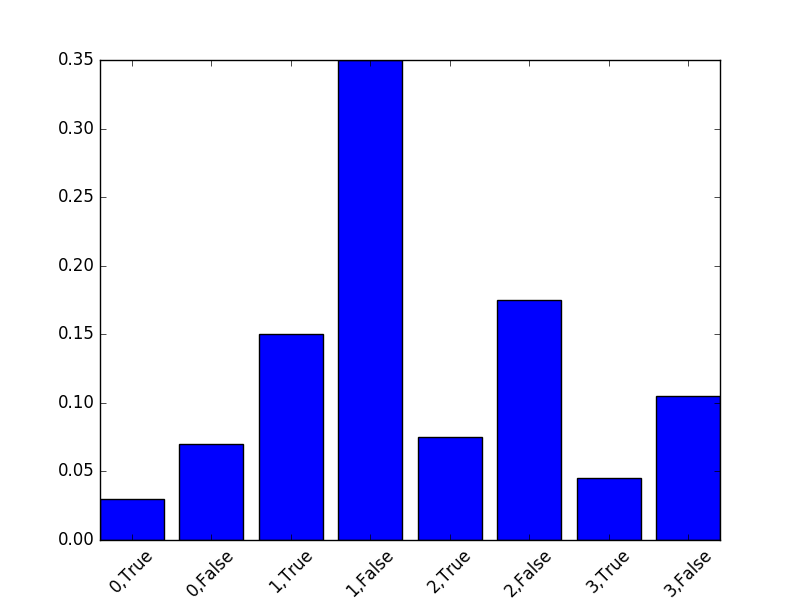
\includegraphics[width=!,totalheight=!,scale=0.35]{Pictures/product_flip.png}
\hspace*{1em}
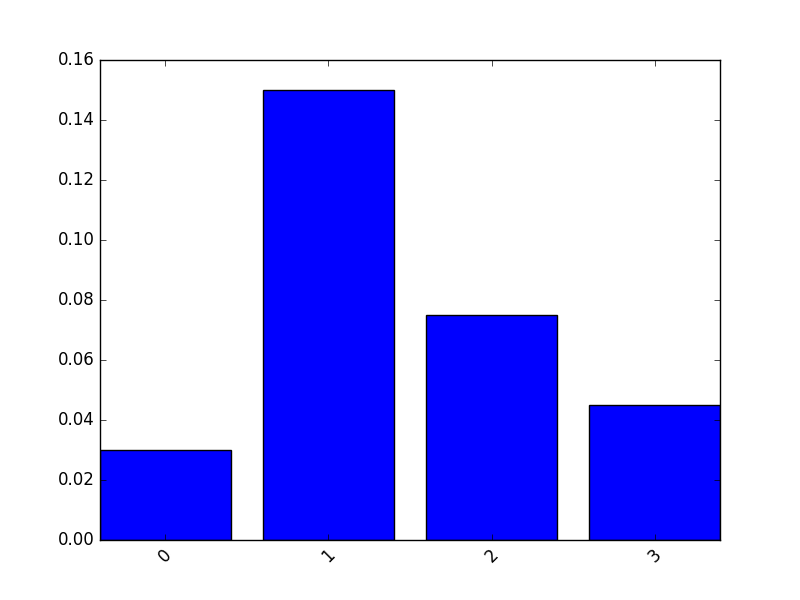
\includegraphics[width=!,totalheight=!,scale=0.35]{Pictures/product_flip_slice.png}
\end{gather*}



\subsection{An excursion on domains of states}\label{subsec:ddomain}

The domain of distribution is a list of `things' that can be
made visible via the \pythoninline{dom} attribute of a state:
\begin{python}
>>> flip(0.8).dom
[True, False]
\end{python}

\noindent If we ask for the domain of a product state we get the
combination of their domains, printed via \pythoninline{*} as:
\begin{python}
>>> (flip(0.8) @ uniform_state(range(5))).dom
[True, False] * range(0, 5)
\end{python}

\noindent You can go one level deeper and ask for the 
discrete domain; it yields a list of domains:
\begin{python}
>>> (flip(0.8) @ uniform_state(range(5))).dom.disc
[[True, False], range(0, 5)]
\end{python}

So far we have constructed joint states only via the product
operator \pythoninline{@}. But we can also defined them directly,
as in:
\begin{python}
>>> s = State([0.1,0.1,0.1,0.7], [[True,False], [0,1]])
>>> s
0.1|True,0> + 0.1|True,1> + 0.1|False,0> + 0.7|False,1>
\end{python}

\noindent This is relevant especially if we wish to define
a non-entwined state.





\section{Predicates}\label{sec:dpred}

Predicates in logic are statements about some space/domain of
elements, such as $x \geq 5$, where $x$ is a variable that ranges for
instance over the domain of natural or real numbers. In predicate
logic predicates are standardly interpreted as \emph{subsets} 
$S\subseteq X$ of a given space $X$.  In the present context we call
such predicates
\emph{sharp}.\index{sharp~predicate!discrete~--}\index{predicate!sharp~discrete~--}
They can be identified with their `characteristic' function $\indic{S}
\colon X \rightarrow \{0,1\}$ given by $\indic{S}(x) = 1$ iff $x\in
S$.  Here, in probabilistic logic, we shall use a more general notion
of predicate,\index{predicate!discrete~--} given by a function
$p\colon X \rightarrow [0,1]$, where $[0,1] \subseteq \RN$ is the unit
interval. Sharp predicate are obviously included in this more general
`fuzzy' notion of predicate.  In a probabilistic setting a sharp
predicate is often called an \emph{event}.\index{event}

The collection of sharp predicates on a set $X$ has a certain
algebraic/logical structure, captured by the notion of a Boolean
algebra. There are truth and falsity predicate $\one, \zero, X
\rightarrow \{0,1\}$ given by the functions which are always $1$, or
always $0$. Also there is negation, written as $\ortho p$, and defined
by $(\ortho p)(x) = 1 - p(x)$. Clearly, $\ortho\ortho p = p$,
$\ortho\one = \zero$ and $\ortho\zero = \one$. In addition, there is
conjuction of predicates $p\wedge q$ given by pointwise
multiplication: $(p \wedge q)(x) = p(x) \cdot q(x)$.

These logical operations do not only work for sharp predicate $X
\rightarrow \{0,1\}$ but for non-sharp $X \rightarrow [0,1]$ as well.
But in that case we do not get a Boolean algebra, but what is called
an \emph{effect module}\cite{Jacobs15}.\index{effect!module} Here it
does not directly matter what the general laws of an effect module
are; it suffices to know the relevant operations on predicates $X
\rightarrow [0,1]$.  Besides negation $\ortho{}$, truth and falsity,
there are two more operation in an effect module that we have not yet
mentioned, namely:
\begin{itemize}
\item partial sum $p+q$ of predicates $p,q$; it is defined if $p(x) +
  q(x) \leq 1$, for all $x\in [0,1]$, and in that case it is determined
  as pointwise addition: $(p+q)(x) = p(x) + q(x)$;

\item scalar multiplication $r\cdot p$, where $r\in [0,1]$ is a
  `probabilistic scalar' and $p$ is a predicate. The resulting
  predicate $r\cdot p \colon X \rightarrow [0,1]$ is defined by
  $(r\cdot p)(x) = r\cdot p(x)$.
\end{itemize}

Recall that a distribution on a (finite) set $X$ can be identified
with a function $\omega \colon X \rightarrow [0,1]$ that satisfies
$\sum_{x}\omega(x) = 1$. Thus, a state is a predicate, but not the
other way around. A predicate is also a function $p\colon X
\rightarrow [0,1]$, but for predicates there is no requirement that
the probabilities $p(x) \in [0,1]$ add up to one. Although they look
similar, it is important to keep states and predicates apart.
Predicates are closed under certain operations, like scalar
multiplication, which do not exist for states.

In the sequel we shall use two important operations combining a state
$\omega$ and a predicate $p$, namely \emph{validity} $\omega\models
p$, and conditioning $\omega|_{p}$. But first we describe the basic
`effect module' operations on predicates in the \EfProb library.


\subsection{Operations on predicates}\label{subsec:dpred:operations}

In this section we discuss the following operations on predicates.
\begin{itemize}
\item orthosupplement, or negation \pythoninline{\~}

\item scalar multiplication \pythoninline{*}

\item partial sum \pythoninline{+}

\item parallel conjunction \pythoninline{@}

\item sequential conjunction \pythoninline{\&}
\end{itemize}

\noindent But first we mention a few ways to obtain predicates in the
first place.

Predicates in \EfProb have a domain, exactly like states have a
domain. We sometimes say that \pythoninline{p} is a predicate on state
\pythoninline{s} if \pythoninline{p} and \pythoninline{s} have the
same domain. This will be most relevant when we discuss validity and
conditioning later on, but it is good to have this idea already in
mind now.

A (discrete) predicate is given by a domain together with
a probability in $[0,1]$ for each of the domain elements.
These probabilities are listed first, as in:
\begin{python}
>>> p = Predicate([0.2, 1, 0.5, 0.0], ['a', 'b', 'c', 'd'])
>>> p
a: 0.2 | b: 1 | c: 0.5 | d: 0
\end{python}

\noindent When printed, these domain elements are enumerated together
with the associated probability.

There are several predefined predicates. The truth predicate on the
domain \pythoninline{[True,False]} is described as:
\begin{python}
>>> truth([True, False])
True: 1 | False: 1
\end{python}

\noindent Similarly, we can describe for instance the falsity
predicate on the domain of the dice distribution:
\begin{python}
>>> falsity([1,2,3,4,5,6])
1: 0 | 2: 0 | 3: 0 | 4: 0 | 5: 0 | 6: 0
\end{python}

\noindent It is useful to have
a predicate which is $1$ only at one element of its domain.
This predicate
is called \pythoninline{point\_pred}. It is illustrated in:
\begin{python}
>>> point_pred(3, range(4))
0: 0 | 1: 0 | 2: 0 | 3: 1
\end{python}

\noindent In the previous section we have seen a function
\pythoninline{random_state}. There is a similar random-predicate
function --- but this time the probabilities do not add up to one.
\begin{python}
>>> random_pred(range(5))
0: 0.806 | 1: 0.593 | 2: 0.758 | 3: 0.68 | 4: 0.442
\end{python}

\noindent Each time this function is called, different probabilities
appear.

As mentioned in the beginning of this section, each state is a
predicate --- but not the other way around. In the \EfProb library
the casting of a state to a predicate can be done via an explicit
method on states, called \pythoninline{as\_pred}.
\begin{python}
>>> s = flip(0.75)
>>> s
0.75|True> + 0.25|False>
>>> s.as_pred()
True: 0.75 | False: 0.25
\end{python}

\noindent We shall make only limited use of this
\pythoninline{as\_pred} method. In our experience it works well to
define predicates directly, instead of via states.

In the remainder of this section we describe operations on predicates.

\paragraph{Orthosupplement} 
As described in the beginning of this section, the
orthosupplement\index{orthosupplement!discrete~--} of a predicate $p$
changes all of its probabilities $p(x)$ into $1-p(x)$, for each
element $x$ in the domain, see:
\begin{python}
>>> p = random_pred(range(5))
>>> p
0: 0.15 | 1: 0.803 | 2: 0.132 | 3: 0.819 | 4: 0.855
>>> ~p
0: 0.85 | 1: 0.197 | 2: 0.868 | 3: 0.181 | 4: 0.145
\end{python}

\noindent Obviously, the orthosupplement of truth is falsity; and
taking the orthosupplement twice returns the original predicate.


\paragraph{Scalar multiplication}
Each predicate $p$ can be multiplied pointwise by a scalar $r\in
[0,1]$, as in:
\begin{python}
>>> s = flip(0.75)
>>> p = s.as_pred()
>>> p
True: 0.75 | False: 0.25
>>> 0.2 * p
True: 0.15 | False: 0.05
\end{python}

\noindent We see that the result of this scalar
multiplicaiton\index{scalar~multiplication!discrete~--} is no longer a
state. There are some obvious equalities, making \pythoninline{*} a
monoid action, namely $1\scalar p = p$ and $r_{1} \scalar (r_{2}
\scalar p) = (r_{1}\scalar r_{2}) \scalar p$.  In addition, scalar
multiplication with zero yields falsity.

In this way we can define a `uniform' predicate, says with domain
\pythoninline{range(6)} and constant value \pythoninline{0.3}, as:
\begin{python}
>>> 0.3 * truth(range(6))
0: 0.3 | 1: 0.3 | 2: 0.3 | 3: 0.3 | 4: 0.3 | 5: 0.3
\end{python}


\paragraph{Partial sum} Pointwise addition of predicates $p,q$ is
only possible when $p(x) + q(x) \leq 1$ for each element $x$ of the
domain.\sidenote{This condition is not checked in the \EfProb
  library.} In that case we can safely add predicates $p,q$ to form a
partial sum\index{partial~sum!of~discrete~predicates} predicate $p+q$,
as in:
\begin{python}
>>> point_pred(3,range(4)) + point_pred(0,range(4))
0: 1 | 1: 0 | 2: 0 | 3: 1
\end{python}

\noindent The sum of predicates \pythoninline{p} and
\pythoninline{\~p} always exists and yields the (constant 1) truth
predicate.

It is not hard to see that predicates, like states are closed under
convex combinations. With the sum operator \pythoninline{+} we can
write such combinations simply as:
\begin{python}
>>> 0.3 * truth(range(4)) + 0.7 * point_pred(0,range(4))
0: 1 | 1: 0.3 | 2: 0.3 | 3: 0.3
\end{python}


\paragraph{Parallel conjunction}
Recall from Subsection~\ref{subsec:dstate:operations} that states can
be put in parallel with the operator \pythoninline{@}. Similarly, if
we have predicates \pythoninline{p1} on state \pythoninline{s1} and
\pythoninline{p2} on state \pythoninline{s2}, then \pythoninline{p1 @
  p2} is a predicate on \pythoninline{s1 @ s2}. Below is an example of
such a parallel
conjunction\index{parallel~conjunction!of~discrete~predicates}
predicate predicate, together with its domain.
\begin{python}
>>> p = Predicate([0.2, 0.8, 0.5, 0.0], ['a', 'b', 'c', 'd'])
>>> q = truth([True,False])
>>> p @ q
a,True: 0.2 | a,False: 0.2 | b,True: 0.8 | b,False: 0.8 | 
   c,True: 0.5 | c,False: 0.5 | d,True: 0 | d,False: 0
>>> (p @ q).dom
['a', 'b', 'c', 'd'] * [True, False]
\end{python}

\noindent Thus, the domain is the cartesian product of the underlying
domains; and the probability on a tuple in this cartesian product is
the product of the probabilities on the tuples. For this reason,
the following predicates are the same:
$$\begin{array}{ccccc}
\mbox{\pythoninline{(r * p) @ q}}
& \qquad &
\mbox{\pythoninline{r * (p @ q)}}
& \qquad &
\mbox{\pythoninline{p @ (r * q)}}
\end{array}$$

\noindent If the sum \pythoninline{p1 + p2} is defined, the following
predicates are also the same.
$$\begin{array}{ccc}
\mbox{\pythoninline{(p1 + p2) @ q}}
& \qquad &
\mbox{\pythoninline{(p1 @ q) + (p2 @ q)}}
\end{array}$$

\noindent Similarly, \pythoninline{@} preserves \pythoninline{+} in
its second argument.


\paragraph{Sequential conjunction}
In contrast to parallel conjunction \pythoninline{@}, sequential
conjunction\index{sequential~conjunction!of~discrete~predicates}
\pythoninline{\&} requires that the two predicates involved have the
same domain. The result is the obtained by the pointwise
multiplication of the probabilities on each domain element:
\begin{python}
>>> p1 = Predicate([0.3, 0.8, 0.01], ['x', 'y', 'z'])
>>> p2 = Predicate([0.5, 0.2, 0.25], ['x', 'y', 'z'])
>>> p1 & p2
x: 0.15 | y: 0.16 | z: 0.0025
>>> (p1 & p2).dom
['x', 'y', 'z']
\end{python}

\noindent This conjunction operator \pythoninline{\&} is commutative
and has truth as neutral element. It preserves sums \pythoninline{+}
in each argument separately.\marginnote[-2\baselineskip]{In quantum
  logic, this operator \pythoninline{\&} is \emph{not} commutative and
  corresponds to `and-then'; there it really makes sense to call
  \pythoninline{\&} \emph{sequential} conjunction, see
  Subsection~\ref{subsec:qpred:operations}. In the current setting of
  discrete (and continuous) probability we use the same name for
  consistency. An additional advantage of calling \pythoninline{\&}
  `sequential conjunction' --- instead of just `conjunction' --- is
  that this name is clearly different from `parallel conjunction'
  \pythoninline{@}.}

Using sequential conjunction \pythoninline{\&} we can define
disjunction\index{disjunction} \pythoninline{|} as its 
De Morgan dual:
$$\begin{array}{ccc}
\mbox{\pythoninline{p | q}}
& \qquad\mbox{is}\qquad &
\mbox{\pythoninline{\~( \~p \& \~q )}}
\end{array}$$



\subsection{Validity}\label{subsec:dpred:validity}

For a state $\omega = \sum_{i} r_{i}\ket{x_i}$ with domain $X$
and a predicate $p\colon X \rightarrow [0,1]$ one can define
the validity\index{validity!discrete~--} $\omega\models p$ of
predicate $p$ in state $\omega$. This validity $\omega\models p$ is
a number in the unit interval $[0,1]$ defined as:
\begin{equation}
\label{eqn:dvalidity}
\begin{array}{rcl}
\omega\models p
\;=\;
\sum_{i}\, r_{i} \cdot p(x_{i}).
\end{array}
\end{equation}

\noindent This number describes the expected value of $p$ in $\omega$.

In \Python the operator \pythoninline{|=} already has a fixed
meaning. We shall use instead \pythoninline{>=} for validity, since it
looks reasonably similar to $\models$. Let a state \pythoninline{s}
have a domain with $n$ elements, with corresponding probabilities
$s_{i}$, for $0\leq i < n$, where $\sum_{i}s_{i} = 1$. Similarly, let
a predicate \pythoninline{p} have the same domain with $n$ elements,
with probabilities $p_{i}$. The validity \pythoninline{s >= p} is then
given by the formula $\sum_{i} s_{i}\cdot p_{i}$. More abstractly, it
is the matrix product $p^{T}\cdot s$, where $p^T$ is the transpose of
$p$.

Here is an example, using the (fair) dice state
\pythoninline{fdice} from Section~\ref{sec:dstate} and the predicates
`even' and `odd', telling whether the number of dots is even or odd.
\begin{python}
>>> fdice = uniform_state([1,2,3,4,5,6])
>>> even = Predicate([0,1,0,1,0,1], [1,2,3,4,5,6]))
>>> odd = ~even
>>> fdice >= even
0.5
>>> fdice >= odd
0.5
>>> fdice >= even + odd
1.0
>>> fdice >= even & odd
0.0
>>> fdice >= even | odd
1.0
\end{python}

\noindent We see that sum \pythoninline{+} and disjunction
\pythoninline{|} give the same outcome. This is because the predicates
\pythoninline{even} and \pythoninline{odd} are sharp. In general there is
a difference, see \eg:
\begin{python}
>>> fdice >= (0.5 * even + 0.2 * odd) + even
0.85
>>> fdice >= (0.5 * even + 0.2 * odd) | even
0.6
\end{python}

\noindent The message is that one should be careful in reading the
logical operators \pythoninline{+} and \pythoninline{|} as `or' in a
probabilistic setting.


Validity $\models$ satisfies some basic mathematical properties:
$$\begin{array}{rcl}
\omega \models \truth
& = &
1
\\
\omega \models \falsity
& = &
0
\\
\omega\models \ortho p
& = &
1 - (\omega\models p)
\\
\omega \models r * p
& = &
r * (\omega\models p)
\\
\omega \models p_{1} + p_{2}
& = &
(\omega\models p_{1}) + (\omega\models p_{2})
\\
\omega \tensor \sigma \models p \tensor q
& = &
(\omega\models p) \cdot (\sigma\models q).
\end{array}$$

\noindent Such properties can be tested (but not proven!) by using
random states and predicates, as in:
\begin{python}
>>> s1 = random_state(range(100))
>>> s2 = random_state(range(50))
>>> p1 = random_pred(range(100))
>>> p2 = random_pred(range(50))
>>> (s1 @ s2) >= (p1 @ p2)
0.25646568531521891
>>> (s1 >= p1) * (s2 >= p2)
0.25646568531521891
\end{python}

The validity \pythoninline{s >= p} is defined only when the state
\pythoninline{s} and the predicate \pythoninline{p} have the same
domain. Often it happens that the domain of the state is `broader'
than the domain of the predicate. In that case we need to `widen' the
predicate. This is called
\emph{weakening}.\index{weakening!of~discrete~predicates} 

More generally, if you have defined a term or a predicate in a context
of assumptions $\Gamma$, then you can also use this same term or
predicate in an enlarged context $\Gamma,\Delta$. Often, weakening is
done implicitly. However, in certain settings weakening requires more
care.
\begin{enumerate}
\item In a \emph{linear} setting, like in linear logic, weakening does
  not exist. In the current setting of quantum logic, we do have
  weakening, since discarding is possible in a quantum
  setting.\sidenote{The companion of weakening is
    \emph{contraction},\index{contraction} making it possible to move
    someting from a context $\Gamma,\Gamma$ to a context
    $\Gamma$. This involves copying of resources, which is not
    possible in a quantum setting, because of
    no-cloning. Semantically, weakening requires projections
    $\Gamma,\Delta \rightarrow \Gamma$, whereas contraction requires
    diagonals $\Gamma \rightarrow \Gamma,\Gamma$.}

\item Usually in logic, weakening is handled automatically, via
  variables, see the the next illustration.
$$\begin{prooftree}
x:A \vdash M(x):B
\justifies
x:A, y:C \vdash M(x):B
\end{prooftree}$$

\noindent The term $M(x)$, depending on variable $x:A$, is weakened to
a larger context with an additional variable $y:B$. In doing so the
term $M$ does not change. This may seem obvious, but in a formalism
without variables, like in the current embedded language \EfProb, we
need to make clear somehow that $M$ has moved.
\end{enumerate}

Here is an example.
\begin{python}
>>> fdice = uniform_state([1,2,3,4,5,6])
>>> even = Predicate([0,1,0,1,0,1], [1,2,3,4,5,6])
>>> fdice >= even
0.5
>>> fdice @ flip(0.3) >= even @ truth([True,False])
0.5
>>> flip(0.3) @ fdice >= truth([True,False]) @ even
0.5
\end{python}

\noindent The predicate \pythoninline{even} can be used as a predicate
on the state \pythoninline{fdice}, but not on the `broader' states
\pythoninline{fdice @ flip(0.3)} or on \pythoninline{flip(0.3) @
  fdice}. However, the predicate \pythoninline{even} can be widened to
these product states, via parallel conjunction \pythoninline{@} with
\pythoninline{truth}, on the right or on the left. Notice that we do
have to provide the \pythoninline{truth} predicate with the right
domain.

Weakening involves some bookkeeping, see for instance
Example~\ref{ex:churchmedical} below. It is not difficult, but one has
to be aware of it, in order to avoid error messages. The conclusion is:
\begin{quote}
Weakening of a predicate works via parallel conjunction with truth,
either on the left or on the right. One then extends the type of a
predicate so that it matches a larger state, without affecting the
validity of the predicate.
\end{quote}




\subsection{Conditioning}\label{subsec:dpred:conditioning}

Conditional probability deals with probabilities `given some
event'. In effectus theory and in the \EfProb library one can
condition a state with a predicate. We start with an illustration,
using the familiar fair dice:
\begin{python}
>>> fdice = uniform_state([1,2,3,4,5,6])
>>> even = Predicate([0,1,0,1,0,1], [1,2,3,4,5,6])
>>> atmost4 = Predicate([1,1,1,1,0,0], [1,2,3,4,5,6])
>>> fdice >= even
0.5
>>> fdice >= atmost4
0.66666666666666667
\end{python}

\noindent Now suppose that we wish to know the probability of
\pythoninline{even}, given that the outcome is at most 4. This
is obtained as:
\begin{python}
>>> fdice / atmost4 >= even
0.5
\end{python}

\noindent The state \pythoninline{fdice / atmost4} is a
\emph{conditional}\index{conditional!state!discrete~--} state,
obtained from \pythoninline{fdice} via conditioning. The probabilities
in \pythoninline{fdice} are updated in the light of the predicate
\pythoninline{atmost4}. Explicitly,
\begin{python}
>>> fdice / atmost4
0.25|1> + 0.25|2> + 0.25|3> + 0.25|4> + 0|5> + 0|6>
\end{python}

\noindent We see that the domain elements \pythoninline{5} and
\pythoninline{6} have probability \pythoninline{0} --- since the
predicate \pythoninline{atmost4} is false for \pythoninline{5} and
\pythoninline{6} --- and that the probabilities of the other elements
--- for which \pythoninline{atmost4} does hold --- have been
normalised, so that they add up to one. It may be clear that in this
conditional, updated state \pythoninline{fdice / atmost4} the
probability of getting an even number of dots is $\frac{1}{2}$.

Similarly:
\begin{python}
>>> fdice / even
0|1> + 0.333|2> + 0|3> + 0.333|4> + 0|5> + 0.333|6>
>>> fdice / even >= atmost4
0.66666666666666667
\end{python}


\begin{remark}
\label{rem:conditionalnotation}
We make the difference explicit between the traditional notation used
in conditional probability (on the left below), and the one that we
use (on the right).
$$\Prob{\mbox{\pythoninline{even | atmost4}}}
\qquad\mbox{and}\qquad
\mbox{\pythoninline{fdice / atmost4 >= even}}$$

\noindent We note the following.
\begin{enumerate}
\item In our notation the underlying state (\pythoninline{fdice}) is
  written explicitly, whereas it is left implicit in the traditional
  notation.

\item Our notation explicitly writes the modification of this state.
  The conditioned state \pythoninline{fdice / atmost4} is useful in
  itself, for instance in conditional expectation, see
  Section~\ref{sec:drandvar}.

\item The traditional notation uses the probability expression
  $\Prob{-}$ which is applied to events. Hence it suggests that its
  argument \pythoninline{even | atmost4} is an event, and thus that
  \pythoninline{|} is an operation on events. This suggestion is
  misleading. Conditioning is an operation between states and
  predicates (events, if you like), and not between two events.
\end{enumerate}
\end{remark}


Here is the mathematical account, see\cite{Jacobs17a} for details. Let
$\omega$ be a state and $p$ a predicate, both with domain $X$. If the
validity $\omega\models p$ is non-zero, one can form the
conditional\index{conditional!state!discrete~--} state $\omega|_{p}$,
which is written in \Python as $\omega/p$. This new state is an update
of $\omega$, given the evidence $p$.  This conditional state
$\omega|_{p}$ is defined by the formula:
\begin{equation}
\label{eqn:dconditiong}
\begin{array}{rcl}
\omega|_{p}
& = &
\displaystyle\sum_{x\in X} \frac{\omega(x)\cdot p(x)}{\omega\models p}
   \bigket{x}.
\end{array}
\end{equation}

\noindent Thus, $\omega|_{p}$ is a normalised product of $\omega$ and
$p$, where normalisation happens via dividing by the validity
$\omega\models p$.

Conditioning is a fundamental operation that forms the basis of
(statistical) learning: updating one's knowledge, in the form of
probabilities of domain elements, in the light of evidence, given by a
predicate.

Conditioning satisfies the following basic equations.
$$\begin{array}{rclcrcccl}
\omega|_{\one}
& = &
\omega
& \qquad\mbox{and}\qquad &
\big(\omega|_{p}\big)|_{q}
& = &
\omega|_{p\andthen q}
& = &
\big(\omega|_{q}\big)|_{p}.
\end{array}$$

\noindent In addition there is Bayes'\index{Bayes'~rule!discrete~--}
rule:
\begin{equation}
\label{eqn:dbayes}
\begin{array}{rcl}
\omega|_{p} \models q
& \;=\; &
\displaystyle\frac{\omega\models p\andthen q}{\omega\models q}.
\end{array}
\end{equation}

\noindent Further, for a predicates \pythoninline{p} on state
\pythoninline{s} and \pythoninline{q} on \pythoninline{t} one
can do conditioning component-wise via weakening:
$$\begin{array}{rcl}
\mbox{\pythoninline{(s @ t) / (p @ truth(t.dom))}}
& \qquad\mbox{is}\qquad &
\mbox{\pythoninline{(s / p) @ t}}
\\
\mbox{\pythoninline{(s @ t) / (truth(s.dom) @ q)}}
& \qquad\mbox{is}\qquad &
\mbox{\pythoninline{s @ (t / q)}}
\end{array}$$

\noindent Here is an illustration.
\begin{python}
>>> s = random_state(range(2))
>>> t = random_state(range(3))
>>> p = random_pred(range(2))
>>> (s @ t) / (p @ truth(t.dom))
0.131|0,0> + 0.161|0,1> + 0.266|0,2> + 0.104|1,0> + 0.127|1,1> + 0.21|1,2>
>>> (s / p) @ t
0.131|0,0> + 0.161|0,1> + 0.266|0,2> + 0.104|1,0> + 0.127|1,1> + 0.21|1,2>
\end{python}


\begin{example}
\label{ex:churchmedical}
The following example\sidenote{\label{note:churchmedical}See
  \url{https://probmods.org/conditioning.html\#example-causal-inference-in-medical-diagnosis}
  for the original description.} is copied from the probabilistic
programming language Church\cite{GoodmanMRBT08}\index{Church} and
translated to the current context. The example involves a number of
diseases:
\begin{itemize}
\item \pythoninline{LC} = lung-cancer, with a priori probability $0.01$;
\item \pythoninline{TB} = tuberculosis, with a priori $0.005$;
\item \pythoninline{CO} = cold, a priori $0.2$;
\item \pythoninline{SF} = stomach-flu, with $0.1$;
\item \pythoninline{OT} = other, also with $0.1$ a priori probability.
\end{itemize}

\noindent We incorporate these five a priori probabilities in a single
product state:
\begin{python}
>>> prior = flip(0.01) @ flip(0.005) @ flip(0.2) @ flip(0.1) @ flip(0.1)
\end{python}

\noindent The above five diseases are translated into five predicates on
this state, each addressing the appropriate component of the above
state, via weakening:
\begin{python}
>>> up = Predicate([1,0], [True,False])
>>> W = truth([True,False])

>>> LC = up @ W @ W @ W @ W
>>> TB = W @ up @ W @ W @ W
>>> CO = W @ W @ up @ W @ W
>>> SF = W @ W @ W @ up @ W
>>> OT = W @ W @ W @ W @ up
\end{python}

\noindent By construction, the validity \pythoninline{prior >= LC} is
\pythoninline{0.01}, and similarly for the other diseases.

Next, one considers the following four symptom predicates, depending
diseases.\marginnote{A discussion about the `logical' description that is
used here, in contrast to a `channel' description may be found later
on, in Example~\ref{ex:bayesianmodeling}.}
\begin{python}
>>> cough = 0.5 * CO | 0.3 * LC | 0.7 * TB |  0.01 * OT
>>> fever = 0.3 * CO | 0.5 * SF | 0.2 * TB | 0.01 * TB
>>> chest_pain = 0.4 * LC | 0.5 * TB | 0.01 * OT
>>> short_breath = 0.4 * LC | 0.5 * TB | 0.01 * OT
\end{python}

\noindent The scalar multiplications in these formulas serve as
``noisy-logical functions to describe the dependence of symptoms on
disease''.

Suppose we observe all these sympotoms. Then we can update
the state to:
\begin{python}
>>> post = prior / (cough & fever & chest_pain & short_breath)
\end{python}

\noindent The question that is asked (the `query') in the original
Church example is: what are the probabilities of the combinations lung
cancer (LC) and tuberculosis (TC), given these observed symptoms? This
is a typical conditional probability problem. The solution is obtained
by taking the appropriate marginals of the conditional state:
\begin{python}
>>> post % [1, 1, 0, 0, 0] 
0.0161|True,True> + 0.242|True,False> + 0.741|False,True> + 0.000919|False,False>
\end{python}

The distribution can also be obtained with Curch at the website
mentioned in sidenote~\ref{note:churchmedical}. The resulting picture
is included in the
margin.\marginnote{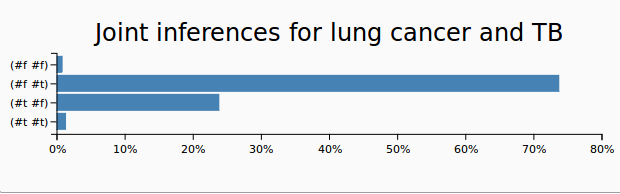
\includegraphics{Pictures/church-medical.png}}
Its True/False options correspond to the above ones, when read from
below. Generating this distribution via Church with 100 samples takes
about 20 seconds. It varies widely, as one can see by trying a few
times at the website. In contrast, our answer pops up in a fraction of
a second and is `exact', in the sense that it does not depend on
sampling but on the probabilistic computation.
%% \mycomment[K]{%
%% Anglican works for this much better,
%% though it's still not easy to obtain accurate values.
%% For some reason this example seems rather difficult for sampling-based approach.}

Instead of using the above marginal distribution, we could also
have asked for the validity of the two relevant attributes, as in:
\begin{python}
>>> post >= LC & TB
0.0161267427839
\end{python}

This medical example illustrates how one builds and analyses models in
the current setting:
\begin{itemize}
\item a `prior' state is defined that incorporates the prior
  probabilities;

\item predicates on this state capture the evidence;

\item observations translate into conditioning of the state;

\item queries are answered either by inspecting the posterior states
  directly, or by asking for specific validities in those states.
\end{itemize}
\end{example}


The following example illustrates another useful observation:
conditioning can introduce entwinedness. 

% Conditioning can also make states non-entwined, see the standard
% examples in Bayesian networks about blocking influence, given some
% evidence.


\begin{example}
\label{ex:entwinednessviaconditioning}
Consider the non-entwined joint state \pythoninline{s} below,
the predicate \pythoninline{p}, and the conditional state 
\pythoninline{t}. This \pythoninline{t} is entwined, since
it is not the product of its marginals:
\begin{python}
>>> s = flip(0.6) @ flip(0.8)
>>> s 
0.48|True,True> + 0.12|True,False> + 0.32|False,True> + 0.08|False,False>
>>> p = Predicate([1, 1, 1, 0], s.dom)
>>> t = s / p
>>> t 
0.522|True,True> + 0.13|True,False> + 0.348|False,True> + 0|False,False>
>>> (t % [1,0]) @ (t % [0,1])
0.567|True,True> + 0.0851|True,False> + 0.302|False,True> + 0.0454|False,False>
\end{python}

\noindent The fact that the state \pythoninline{t} is entwined can
also be deduced from~\eqref{eqn:entwined}.
\end{example}


\begin{example}
\label{ex:dtotalprobability}
This example illustrates the law of total
probability\index{law~of~total~probability}\index{probability!law~of~total~--}
in the current setting. We start from an arbitrary state and predicate
and the associated validity:
\begin{python}
>>> s = random_state(range(4))
>>> p = random_pred(range(4))
>>> s >= p
0.326073622519
\end{python}

\noindent Next we wish to obtain this same probability via the law of
total probability. This requires a test,\index{test} that is, a set of
predicates that add up to one. We choose a test of length 3. We create
it in the following way, where the scalar \pythoninline{0.5} is used
to ensure that the scaled predicates \pythoninline{0.5 * q1} and
\pythoninline{0.5 * q2} are orthogonal (summable).  The predicate
\pythoninline{q3} is then determined so that \pythoninline{q1 + q2 +
  q3} equals the truth predicate.
\begin{python}
>>> q1 = 0.5 * random_pred(range(4))
>>> q2 = 0.5 * random_pred(range(4))
>>> q3 = ~(q1 + q2)
>>> (s / q1 >= p) * (s >= q1) + (s / q2 >= p) * (s >= q2) +  (s / q3 >= p) * (s >= q3)
0.326073622519
\end{python}

\noindent This last formula is equivalent, by Bayes'
rule~\eqref{eqn:dbayes}, to:
\begin{python}
>>> (s >= q1 & p) + (s >= q2 & p) + (s >= q3 & p)
0.326073622519
\end{python}

\noindent In discrete and continuous probability such tests can be be
factored out. But this is not the case in quantum probability, see at
the end of Example~\ref{ex:polarisation}.
\end{example}


\section{Random variables}\label{sec:drandvar}

Random variables are used in probability theory to map elements of the
sample space (domain) to real numbers. Given a state on the domain,
one can then comppute the expected value, or variance. Here is a
simple example where this is useful.
\begin{quote}
If it rains, an umbrella sales person can earn \euro{100} per day. If
it is a fair weather day (s)he can lose \euro{20} per day. What is the
expected return if the probability of rain is 0.3?
\end{quote}

\noindent In an example like this it is important first to look for
the state. Here model it as \pythoninline{flip(0.3)}, with domain
\pythoninline{[True,False]}, describing whether or not it is
raining. We would like to map the domain element \pythoninline{True}
to \pythoninline{100} and the domain element \pythoninline{False} to
\pythoninline{-20}. This is achieved in \EfProb via:
\begin{python}
>>> rain_state = flip(0.3)
>>> umbrella_sales_rv = RandVar([100, -20], [True,False])
>>> umbrella_sales_rv.exp(rain_state)
16.0
\end{python}

\noindent We see that a random variable is defined by a list and a
domain (also a list). The first list gives the real number values
corresponding to the elements of the domain. A random variable has an
expectation\index{expectation!discrete~--} method \pythoninline{exp},
which takes a state as argument. This state must have the same domain
as the random variable. In a similar way one obtains the
variance\index{variance!discrete~--} or standard
deviation\index{standard~deviation!discrete~--} via the methods
\pythoninline{var} and \pythoninline{stdev}.

Here is another example of a random variable, now defined on (the
domain of) the product state of a pair of dices. Instead of using a
list, we use a function as first argument. It maps a pair $(x,y) \in
\{1,2,3,4,5,6\} \times \{1,2,3,4,5,6\}$ to the sum $x+y$.
\begin{python}
>>> fdice = uniform_state([1,2,3,4,5,6])
>>> twodice = fdice @ fdice
>>> sum_rv = RandVar.fromfun(lambda x,y: x+y, twodice.dom)
>>> sum_rv.exp(twodice)
7.0
\end{python}

% Alternative: RandVar(lambda *xs: xs[0] + xs[1], twodice.dom)

The \EfProb framework also supports \emph{conditional}
expectation,\index{conditional!expectation!discrete~--} simply via
conditional states. For instance, the expected sum values of two dices
given that both of them are even (or odd) are:
\begin{python}
>>> even = Predicate([0,1,0,1,0,1], [1,2,3,4,5,6])
>>> odd = ~even
>>> sum_rv.exp( twodice / (even @ even) )
8.0
>>> sum_rv.exp( twodice / (odd @ odd) )
6.0
\end{python}

% double check of even case
%
% 1/9*(2+2) + 1/9*(4+4) + 1/9*(6+6) + 2/9*(2+4) + 2/9*(2+6) + 2/9*(4+6)
% = 4/9 + 8/9 + 12/9 + 12/9 + 16/9 + 20/9 = 72/9 = 8

We can use \Python as `meta-language' to define for instance
a function that returns the expected value of \pythoninline{n}
dices:
\begin{python}
>>> def sums_exp(n): return RandVar.fromfun(lambda *xs: sum(xs), 
... (fdice ** n).dom).exp(fdice ** n)
>>> sums_exp(1)
3.5
>>> sums_exp(2)
7.0
>>> sums_exp(3)
10.5
>>> sums_exp(8)
28.000000000186169
\end{python}

\noindent The latter computation takes in the order of 15 seconds on
an ordinary laptop. The domain has size $6^{8} = 1.679.616$
elements.\marginnote{One sees a pattern emerging, namely that
  \pythoninline{sums\_exp(n)} equals \pythoninline{3.5 * n}. However,
  such formulas cannot be proven within \EfProb. It can only be
  tested, for small numbers.} The function involved uses a \Python
trick for arbitrary-length sequences of arguments, namely by adding a
star in \pythoninline{lambda *xs: sum(xs)}.

Below is a variation where we look at the `conditional' expected value
for \pythoninline{n} dices with \pythoninline{even} outcome, via
conditional states.\marginnote[3\baselineskip]{Here the pattern is
  \pythoninline{even\_sums\_exp(n)} equals \pythoninline{4 * n}.}
\begin{python}
>>> def even_sums_exp(n): return RandVar.fromfun(lambda *xs: sum(xs), 
... (fdice ** n).dom).exp( (fdice ** n) / (even ** n) )
... 
>>> even_sums_exp(1)
4.0
>>> even_sums_exp(2)
8.0
>>> even_sums_exp(8)
32.0
\end{python}

As described above, random variables are functions from a domain to
real numbers. This means that we can define various operations like
sum, product, scalar multiplication on random variable by applying
these operations point-wise. Such operations on random variables are
pre-defined in \EfProb.

\marginpar{Todo: relation between predicates and random variables}



\section{Channels}\label{sec:dchannel}

There are several ways to understand
channels,\index{channel!discrete~--} in discrete probability, namely
as:
\begin{itemize}
\item stochastic matrices;

\item probabilistic transition systems;

\item conditional probability tables, in Bayesian networks;

\item indexed collections of states with the same domain;

\item Kleisli maps for the distribution monad $\Dst$, between finite
  sets.
\end{itemize}

\noindent Channels form an abstraction notion of `map' in a
probabilistic setting, not only in discrete, but also in continuous
and in quantum probability. They can be used for forward state
transformation and backward predicate transformation. They can be
composed both sequentially and parallelly, and form the basic
ingredients of a probabilistic programming language.

Since channels are maps, they have a \emph{domain} and a
\emph{codomain}. These (co)domains are precisely as for states and
predicates. We often write \pythoninline{c : dom -> cod} to indicate
that \pythoninline{c} is a channel with domain \pythoninline{dom} and
codomain \pythoninline{cod}. These domain and codomain of a channel
\pythoninline{c} can be obtained via attributes \pythoninline{c.dom}
and \pythoninline{c.cod}.

We shall see several ways to define channels.
\begin{itemize}
\item Channels can be defined via (stochastic) matrix, provided with a
  domain and codomain; this is illustrated in
  Examples~\ref{ex:diseasetest} and~\ref{ex:genetic} below.

\item There are also special `conditional probability table' functions
  which are convenient to define channels associated with a Bayesian
  Network, see Examples~\ref{ex:paperacceptance}
  and~\ref{ex:bayesianmodeling}.

\item A channel can also be obtained from a list of states, all with
  the same domain. This is done via a static method
  \pythoninline{from\_states}, as in:
\begin{python}
>>> c = Channel.from_states([flip(0.2), flip(0.3), flip(0.5)])
>>> c
Channel of type: range(0, 3) --> [True, False]
>>> c.get_state(1)
0.3|True> + 0.7|False>
\end{python}

\noindent We see that when printed, only the domain and codomain of a
channel are shown. This channel maps an element $0 \leq i < 3$ in
\pythoninline{range(0,3)} to the $i$-th state in the list, used as
argument to the function \pythoninline{from\_states}. These states
can be extracted via the \pythoninline{get\_state} method.

\item Such a mapping from elements of a domain to states is a `Kleisli
  map' for the distribution monad $\Dst$, in categorical terminology.
  Given such a mapping, one can form an associated channel. For
  instance, the previous example can also be obtained via the function
  \pythoninline{chan\_fromklmap}.
\begin{python}
>>> d = chan_fromklmap(lambda i: flip(0.2) if i == 0 else
...                    flip(0.3) if i == 1 else flip(0.5), range(3), [True,False])
\end{python}
\end{itemize}




\subsection{State and predicate transformation}\label{subsec:dchannel:statepredtransform}

Let \pythoninline{c} be a channel, with domain \pythoninline{c.dom}.
Each state \pythoninline{s} whose domain \pythoninline{s.dom} is the
same as \pythoninline{c.dom} can be transformed into a state
\pythoninline{c >> s} with domain \pythoninline{c.cod}. We first
describe how such state transformation works. Subsequently we discuss
predicate transformation \pythoninline{c << p}, which works against
the direction of the channel.

For the time being we shall define channels as in
Example~\ref{ex:diseasetest}: a channel from a domain with $n$
elements to a domain with $m$ elements is given by an $n\times m$
stochastic matrix $M$, presented in linear form. The elements $M_{ij}$
of the matrix, for $0 \leq i < n$ and $0 \leq j < m$, satisfy
$\sum_{j}M_{ij} = 1$, for each $i$. Thus, if a state with a domain
with $n$ elements is given by probabilities $s_{i}$, with
$\sum_{i}s_{i} = 1$, then state transformation can be described as
$M\cdot s$, that is, as application of the matrix $M$ to the state
$s$. Explicitly, $(M\cdot s)_{j} = \sum_{i} M_{ij}\cdot s_{i}$.

Predicate transformation works in the other direction. If a predicate
\pythoninline{p} has a domain \pythoninline{p.dom} that is equal to
the codomain \pythoninline{c.cod} of a channel \pythoninline{c}, then
we can form the predicate \pythoninline{c << p} with domain
\pythoninline{c.dom}. It may be understood as the weakest
precondition\index{weakest~precondition!for~discrete~predicates} of
\pythoninline{p} along \pythoninline{c}.  If the channel
\pythoninline{c} has a matrix $M$ as in the previous paragraph, and
predicate \pythoninline{p} involves probabilities $p_j$, then the
pulled back predicate \pythoninline{c << p} has probabilities
$(p^{T}\cdot M)_{i} = \sum_{j} p_{j}\cdot M_{ij}$.

The following general result will be illustrated in
Example~\ref{ex:diseasetest} below. It shows how state- and
predicate-transformation behave appropriately wrt.\ validity, as
expressed by the following transformations validity equation.
\begin{equation}
\label{eqn:dvaliditytransformation}
\begin{array}{rcl}
c \gg s \models p
& \;=\; &
s \models c \ll p.
\end{array}
\end{equation}


\begin{example}
\label{ex:diseasetest}
We start with an illustration of the use of channels, which is typical
for Bayesian reasoning, taken from\cite{JacobsZ16}.  For explanatary
reasons we shall be very explicit about the domains involved. The
setting is given by some disease with a priori probability of
$1\%$. There is a test for the disease with the following
`sensitivity'. If someone has the disease, then the test is $90\%$
positive; but if someone does not have the disease, there is stil a
$5\%$ chance that the test is positive.
\begin{python}
>>> disease_domain = ['D', '~D']
>>> prior = State([1/100, 99/100], disease_domain)
>>> disease_pred = Predicate([1,0], disease_domain)
>>> prior
0.01|D> + 0.99|~D>
>>> prior >= disease_pred
0.01
>>> test_domain = ['T', '~T']
>>> test_pred = Predicate([1,0], test_domain)
>>> sensitivity = Channel([[9/10, 1/20], [1/10, 19/20]], disease_domain, test_domain)
>>> sensitivity.dom
['D', '~D']
>>> sensitivity.cod
['T', '~T']
\end{python}

\noindent The channel can be seen as a map \pythoninline{sensitivity :
  disease\_domain -> test\_domain}. We first use the channel to
compute the probability that a test for an arbitrary person is
positive. This is done via \emph{state transformation}, using the
operator \pythoninline{>>}, as in:
\begin{python}
>>> sensitivity >> prior
0.0585|T> + 0.942|~T>
\end{python}

% 1/100*9/10 + 99/100*1/20 = 9/1000 + 99/2000 = 117/2000

\noindent This probability \pythoninline{0.0585} is the fraction
\pythoninline{117/2000}. Notice that via state transformation
\pythoninline{sensitivity >> prior} the state \pythoninline{prior} on
the disease domain \pythoninline{['D', '~D']} is transformed into a
state on the test domain \pythoninline{['T', '~T']}. State
transformation \pythoninline{>>} happens via a `push forward' in the
direction of the channel.

The a-priori-positive-test probability \pythoninline{117/2000} can
also be obtained via validity \pythoninline{>=} of predicates, in two
different ways:
\begin{python}
>>> sensitivity >> prior >= disease_pred
0.0585
>>> prior >= sensitivity << test_pred
0.0585
\end{python}

\noindent First we ask for the validity of the disease predicate in
the transformed state \pythoninline{sensitivity >>
  prior}. Next we use \emph{predicate transformation}
\pythoninline{<<} to transform the test predicate on domain
\pythoninline{['T', '~T']} into a predicate \pythoninline{sensitivity
  << test\_pred} on the disease domain \pythoninline{['D',
    '~D']}. Thus, in predicate transformation a predicate is `pulled
back', in the opposite direction of the channel. The validity of this
pulled-back predicate is then computed in the prior state. It yields
the same outcome, via the general rule described
in~\eqref{eqn:dvaliditytransformation}.

Once we have this pulled back predicate \pythoninline{sensitivity
  << test\_pred} we can use it to condition the prior state into
a posterior state. A bit pedantically:
\begin{python}
>>> posterior = prior / (sensitivity << test_pred)
>>> posterior
0.154|D> + 0.846|~D>
\end{python}

\noindent This value \pythoninline{0.154} is the truncated fraction
\pythoninline{18/117}. It gives the probability of having the disease,
given a positive test.
\end{example}


Later on, in Example~\ref{ex:paperacceptance} we shall see more
examples of Bayesian networks, also with \EfProb support for defining
the relevant channels from conditional probability
tables\index{conditional!probability~table} (CPTs).

We include another example illustrating how to incorporate hidden
Markov models\index{hidden~Markov~model} as channels.  This example is
adapted from the reference manual of the probabilistic language
BLOG\cite{MilchMRSOK07}.\index{BLOG}


\begin{example}
\label{ex:genetic}
We consider the four types of bases found in a DNA molecule: adenine
(A), cytosine (C), guanine (G), and thymine (T). These four letters A,
C, G, T will be used to form a domain, a prior distribution
\pythoninline{s0} on that domain, and four predicates on
\pythoninline{s0} for the different components.
\begin{python}
>>> ACGT = ['A', 'C', 'G', 'T']
>>> s0 = State([0.3, 0.2, 0.1, 0.4], ACGT)
>>> A = Predicate([1,0,0,0], ACGT)
>>> C = Predicate([0,1,0,0], ACGT)
>>> G = Predicate([0,0,1,0], ACGT)
>>> T = Predicate([0,0,0,1], ACGT)
>>> s0 >= A
0.3
\end{python}

\noindent The transition from one state to a next is given by a channel
\pythoninline{trs}. There is also a channel \pythoninline{obs} that
gives the probability of each predicate in a particular state.
\begin{python}
>>> trs = Channel([[0.1, 0.3, 0.3, 0.3],
...                [0.3, 0.1, 0.3, 0.3],
...                [0.3, 0.3, 0.1, 0.3],
...                [0.3, 0.3, 0.3, 0.1]], ACGT, ACGT)
>>> obs = Channel([[0.85, 0.05, 0.05, 0.05],
...                [0.05, 0.85, 0.05, 0.05],
...                [0.05, 0.05, 0.85, 0.05],
...                [0.05, 0.05, 0.05, 0.85]], ACGT, ACGT)
\end{python}

\noindent The question that is addressed in the BLOG\index{BLOG}
example is the following. Suppose we have consecutive observations: C,
A, A, A, G; what is the resulting state/distribution?

The dynamics of hidden Markov models is given by (1)~update with
observation, (2)~make a transition. This is done consecutively by
using both predicate transformation and state transformation:
\begin{python}
>>> s1 = trs >> (s0 / (obs << C))
>>> s1
0.286|A> + 0.138|C> + 0.295|G> + 0.281|T>
>>> s2 = trs >> (s1 / (obs << A))
>>> s2
0.126|A> + 0.295|C> + 0.289|G> + 0.29|T>
>>> s3 = trs >> (s2 / (obs << A))
>>> s3 
0.148|A> + 0.284|C> + 0.284|G> + 0.284|T>
>>> s4 = trs >> (s3 / (obs << A))
>>> s4
0.158|A> + 0.28|C> + 0.281|G> + 0.281|T>
>>> s5 = trs >> (s4 / (obs << G))
>>> s5
0.295|A> + 0.29|C> + 0.126|G> + 0.29|T>
\end{python}

\noindent Of course, one may handle such a sequence of observations
automatically by iteration.

The above probabilities are the same as the ones in the BLOG reference
manual. An important difference is that they are obtained here in an
`exact' manner, via actual computations, where in BLOG they are
obtained via iterated sampling.
\end{example}



\subsection{Sequential and parallel composition}\label{subsec:dchannel:composition}

Channels can be composed both sequentially and in parallel. For
sequential composition \pythoninline{d * c}, read as
`\pythoninline{d} after \pythoninline{c}', it is required that the
codomain of \pythoninline{c} is equal to the domain of
\pythoninline{d}, as in:
$$\xymatrix{
\mbox{\pythoninline{c.dom}}\ar[r]^-{\mbox{\pythoninline{c}}} &
\mbox{\pythoninline{c.cod = d.dom}}\ar[r]^-{\mbox{\pythoninline{d}}} &
\mbox{\pythoninline{d.cod}}
}$$

\noindent The resulting channel \pythoninline{d * c : c.dom -> d.cod}
is obtained by matrix multiplication. As a result, \pythoninline{*}
is an associative operation, with the identity channel (given by
the identity matrix) as unit element.

Sequential composition of channels interacts with state- and
predicate- transformation in the `obvious' way: the left- and right
hand side below are the same:
\begin{center}
\begin{tabular}{ccc}
\mbox{\pythoninline{(d * c) >> s}}
& \qquad\mbox{is}\qquad\quad &
\mbox{\pythoninline{d >> (c >> s)}}
\\
\mbox{\pythoninline{(d * c) << p}}
& \qquad\mbox{is}\qquad\quad &
\mbox{\pythoninline{c << (d << p)}}
\end{tabular}
\end{center}

\noindent Notice the reversal in order of the channels \pythoninline{c}
and \pythoninline{d} in predicate transformation. The reason is that
predicate transformation works in a backward direction.


For parallel composition \pythoninline{c @ d} of channels
\pythoninline{c}, \pythoninline{d} there are no type
restrictions. Thus we can form:
$$\xymatrix@C+1pc{
\mbox{\pythoninline{c.dom + d.dom}}\ar[r]^-{\mbox{\pythoninline{c @ d}}} &
\mbox{\pythoninline{c.cod + d.cod}}
}$$

\noindent The sum \pythoninline{+} of domains involves a concatenation
of lists of dimensions.

This parallel
composition \pythoninline{@} for channels interacts appropriately with
composition \pythoninline{@} for states and with \pythoninline{@} for
predicates, in the sense that:
\begin{center}
\begin{tabular}{ccc}
\mbox{\pythoninline{(c @ d) >> (s @ t)}}
& \qquad\mbox{is}\qquad\quad &
\mbox{\pythoninline{(c >> s) @ (d >> t)}}
\\
\mbox{\pythoninline{(c @ d) << (p @ q)}}
& \qquad\mbox{is}\qquad\quad &
\mbox{\pythoninline{(c << p) @ (d << q)}}
\end{tabular}
\end{center}

\noindent The `interchange law' for monoidal categories also holds:
\begin{center}
\begin{tabular}{ccc}
\mbox{\pythoninline{(c @ d) * (e @ f)}}
& \qquad\mbox{is}\qquad\quad &
\mbox{\pythoninline{(c * e) @ (d * f)}}
\end{tabular}
\end{center}





\subsection{Structural channels}\label{subsec:dchannel:structural}

There are several channels which we call `structural' because their
main purpose is to provide structure to a network of channels. These
structural channels include identity, discard (and projection), copy,
swap, but also `ancilla' and measure.


\paragraph{Identity channels}
For each domain \pythoninline{dom} there is an identity
channel\index{identity~channel!discrete~---}\index{channel!discrete~identity~--}
\pythoninline{idn(dom) : dom -> dom}. It is given by the identity
matrix. For an arbitrary channel \pythoninline{c : dom -> cod} the
following three channels are the same.
$$\mbox{\pythoninline{idn(cod) * c}}
\qquad\qquad
\mbox{\pythoninline{c}}
\qquad\qquad
\mbox{\pythoninline{c * idn(dom)}}$$

\noindent This says that identity channels are units (`skip') for
sequential composition \pythoninline{*}.

These identity channels seem rather useless, but they turn out to be
handy in parallel compositions like \pythoninline{c @ idn(dom)}.  Two
identity channels in parallel forms itself an identity channel.


\paragraph{Discard channel} For each domain \pythoninline{dom}
there is discard
channel\index{discard~channel!discrete~---}\index{channel!discrete~discard~--}
\pythoninline{discard(dom) : dom -> []}.  It throws away its
input. Again this looks silly. But discard channels, in parallel with
identity channels, give us projection channels. This is illustrated
below, via the projections \pythoninline{proj1} and
\pythoninline{proj2} which can do both
marginalisation\index{marginalisation!via~a~projection~channel} of
states and weakening\index{weakening!via~a~projection~channel} of
predicates.
\begin{python}
>>> s = State([1/12, 1/8, 1/4, 1/4, 1/6, 1/8], [[True,False], range(3)])
>>> s
0.0833|True,0> + 0.125|True,1> + 0.25|True,2> + 0.25|False,0> + 0.167|False,1> + 0.125|False,2>
>>> s % [1,0]
0.458|True> + 0.542|False>
>>> s % [0,1]
0.333|0> + 0.292|1> + 0.375|2>
>>> proj1 = idn([True,False]) @ discard(range(3))
>>> proj2 = discard([True,False]) @ idn(range(3))
>>> proj1 >> s
0.458|True> + 0.542|False>
>>> proj2 >> s
0.333|0> + 0.292|1> + 0.375|2>
\end{python}

\noindent We continue the same example, now illustrating weakening
of predicates via these same projection channels \pythoninline{proj1} and
\pythoninline{proj2}.
\begin{python}
>>> p1 = Predicate([1/4, 5/8], [True,False])
>>> p2 = Predicate([1/2, 1, 1/12], range(3))
>>> p1 @ truth(range(3))
True,0: 0.25 | True,1: 0.25 | True,2: 0.25 | False,0: 0.625 | False,1: 0.625 | False,2: 0.625
>>> truth([True,False]) @ p2
True,0: 0.5 | True,1: 1 | True,2: 0.0833 | False,0: 0.5 | False,1: 1 | False,2: 0.0833
>>> proj1 << p1
True,0: 0.25 | True,1: 0.25 | True,2: 0.25 | False,0: 0.625 | False,1: 0.625 | False,2: 0.625
>>> proj2 << p2
True,0: 0.5 | True,1: 1 | True,2: 0.0833 | False,0: 0.5 | False,1: 1 | False,2: 0.0833
\end{python}

\noindent Now that we know that marginalisation and weakening are
intimately related via state/predicate transformation, we observe that
we can also apply the transformations validity
equation~\eqref{eqn:dvaliditytransformation} and obtain the
following informal equation:
$$\begin{array}{rcl}
\textsf{marginalisation}(\omega) \models p
& \;=\; &
\omega \models \textsf{weakening}(p).
\end{array}$$

\noindent This requires that marginalisation and weakening are
done in the same coordinates. The following illustration continues
the previous example.
\begin{python}
>>> proj1 >> s >= p1
0.453125
>>> s >= proj1 << p1
0.453125
\end{python}


\paragraph{Copy and swap channels} For each domain \pythoninline{dom}
there is a copy
channel\index{copy~channel!discrete~---}\index{channel!discrete~copy~--}
\pythoninline{copy(dom) : dom -> dom + dom}. It duplicates its input.
Such copying exists in classical (discrete and continuous)
probability, but not in quantum probability, because of the so-called
no-cloning result. This copy channels is usef for instance to define
the `graph'\index{graph~of~a~channel} of a channel \pythoninline{c :
  dom -> cod} as a new channel \pythoninline{graph(c) : dom -> dom +
  cod}, in the following way.
\begin{python}
def graph(c):
    return (idn(c.dom) @ c) * copy(c.dom)
\end{python}

\noindent This turns out to be a useful construction.

For each pair of domains \pythoninline{dom1}
and \pythoninline{dom2} there is a swap
channel:\index{swap~channel!discrete~---}\index{channel!discrete~swap~--}
$$\mbox{\pythoninline{swap(dom1,dom2) : dom1 + dom2 -> dom2 + dom1}}$$

\noindent It behaves in the obvious manner. These copy and swap
channels play an important role in the channel that models a Bayesian
network in Example~\ref{ex:paperacceptance}.


\marginpar{To do: channels from states/predicates, case channels}


We conclude this section with an example that illustrates
the use of structural channels. At the same time it illustrates
how entwinedness of states.

\begin{example}
\label{ex:diseasemood}
This examples introduces a variation on the disease-test illustration
from Example~\ref{ex:diseasetest}. There we used a prior disease state:
\begin{python}
>>> disease_domain = ['D', '~D']
>>> prior = State([1/100, 99/100], disease_domain)
\end{python}

\noindent Now we add a second domain for mood, and use joint
state for disease and mood, simply called \pythoninline{prior}.
\begin{python}
>>> mood_domain = ['M', '~M']
>>> joint_prior = State([0.05, 0.5, 0.4, 0.05], [disease_domain, mood_domain])
>>> joint_prior
0.05|D,M> + 0.5|D,~M> + 0.4|~D,M> + 0.05|~D,~M>
\end{python}

\noindent This state describes a low probability for having the
disease and a good mood, and also for not having the disease and a bad
mood. The combination disease and bad mood, and no disease and good
mood is more likely.

We recall from Example~\ref{ex:diseasetest} that there is a test for
the disease, described via a channel \pythoninline{sensitivity}. We
now ask ourselves the question: what are the mood probabilities before
and after a positive test?

The mood before the test is simply the second marginal of the
joint state \pythoninline{joint\_prior}.
\begin{python}
>>> joint_prior % [0,1]
0.45|M> + 0.55|~M>
\end{python}

\noindent We first look at the probability of a positive test in
the joint prior state. There are several equivalent ways to compute
this. The first one takes the first marginal, applies the sensitivity
state transformer and asks for the validity in the resulting state:
\begin{python}
>>> sensitivity >> (joint_prior % [1,0]) >= test_pred
0.5175
\end{python}

\noindent One can also extend the sensitivity channel in parallel
with the identity channel, apply it to the whole joint state, and
look at the validity of the weakened predicate:
\begin{python}
>>> (sensitivity @ idn(mood_domain)) >> joint_prior >= (test_pred @ truth(mood_domain))
0.5175
\end{python}

\noindent But, remembering the transformations validity
equation~\eqref{eqn:dvaliditytransformation}, we note that we can get
this same validity via predicate transformation:
\begin{python}
>>> joint_prior >= (sensitivity @ idn(mood_domain)) << (test_pred @ truth(mood_domain))
0.5175
\end{python}

\noindent The latter can even be simplied to:
\begin{python}
>>> joint_prior >= ((sensitivity << test_pred) @ truth(mood_domain))
0.5175
\end{python}


\noindent Recall that we are interested in the mood after a positive
test. First we update the prior with the information of a positive
test, and then we compute the first and second marginal:
\begin{python}
>>> joint_post = joint_prior / ((sensitivity << test_pred) @ truth(mood_domain))
>>> joint_post % [1,0]
0.957|D> + 0.0435|~D>
>>> joint_post % [0,1]
0.126|M> + 0.874|~M>
\end{python}

\noindent We thus see that, as a result of a positive test, the mood
drops from a prior value of \pythoninline{0.45} to a posterior value
of \pythoninline{0.126}. In itself this is remarkable, since the
sensitivity channel only acts on the first `disease' part of the joint
state, and not on the `mood' part. The influence between these parts
happens because `disease' and `mood' are entwined: the rise in disease
probability leads to a lower mood.
\end{example}



\section{Bayesian networks}\label{sec:bayesiannetwork}

The \EfProb library offers support for modeling Bayesian networks and
for performing certain elementary computations within such
networks. This includes functions to define prior states and
conditional probability tables (cpt's), which are essentially
channels.

A Bayesian network is given by a directed acyclic graph, consisting of
nodes with arrows between them. These nodes can be understood as
probability distributions on a two-element domain, whose elements are
typically written as \pythoninline{t} for true and \pythoninline{f}
for false. Nodes with no incoming arcs are called initial, and
correspond to prior states. Arcs capture conditional probabilities.
This will be explained via a Bayesian network taken
from~\cite{JacobsZ16}.


\begin{example}
\label{ex:paperacceptance}
Consider the Bayesian network below that describes the various aspects
of getting an academic paper accepted at a conference.
\begin{gather*}
\vcenter{\xymatrix@R=1pt@C=12pt{
\ovalbox{\textbf{T}ime}\ar@/^/[ddr]\ar@/^/[r] & \ovalbox{\textbf{W}ell Written}\ar@/^/[ddr]\ar@/^/[r] & \ovalbox{\textbf{P}ositive Reviews} \ar@/^/[dr]
\\
&  & & \ovalbox{\textbf{A}cceptance}
\\
\ovalbox{\textbf{S}kill}\ar@/^/[r] & \ovalbox{Strong \textbf{R}esults} \ar@/^/[uur]\ar@/^/[r] & \ovalbox{\begin{minipage}{2.5cm} \centering PC \textbf{M}ember Championing\end{minipage}} \ar@/^/[ur]
}} \label{eq:acceptanceNetwork} \\
\begin{tabular}{c}
{\setlength\tabcolsep{0.2em}\begin{tabular}{|c|}
\hline
$\Prob{T}$ \\
\hline\hline
$\frac{4}{10}$ \\
\hline
\end{tabular}}
{\setlength\tabcolsep{0.2em}\begin{tabular}{|c|}
\hline
$\Prob{S}$ \\
\hline\hline
$\frac{7}{10}$ \\
\hline
\end{tabular}}
\\[1.5em]
{\setlength\tabcolsep{0.2em}\begin{tabular}{|c|c|}
\hline
$T$ & $\Prob{W}$ \\
\hline\hline
$t$ & $\frac{8}{10}$ \\
\hline
$f$ & $\frac{3}{10}$ \\
\hline
\end{tabular}}
\end{tabular}
\ \
{\setlength\tabcolsep{0.2em}\begin{tabular}{|cc|c|}
\hline
$T$ & $S$ & $\Prob{R}$ \\
\hline\hline
$t$ & $t$ & $\frac{9}{10}$ \\
\hline
$t$ & $f$ & $\frac{6}{10}$ \\
\hline
$f$ & $t$ & $\frac{4}{10}$ \\
\hline
$f$ & $f$ & $\frac{1}{10}$ \\
\hline
\end{tabular}}
\ \
{\setlength\tabcolsep{0.2em}\begin{tabular}{|cc|c|}
\hline
$W$ & $R$ & $\Prob{P}$ \\
\hline\hline
$t$ & $t$ & $\frac{8}{10}$ \\
\hline
$t$ & $f$ & $\frac{5}{10}$ \\
\hline
$f$ & $t$ & $\frac{6}{10}$ \\
\hline
$f$ & $f$ & $\frac{1}{10}$ \\
\hline
\end{tabular}}
\ \
{\setlength\tabcolsep{0.2em}\begin{tabular}{|cc|c|}
\hline
$W$ & $R$ & $\Prob{M}$ \\
\hline\hline
$t$ & $t$ & $\frac{4}{10}$ \\
\hline
$t$ & $f$ & $\frac{1}{10}$ \\
\hline
$f$ & $t$ & $\frac{3}{10}$ \\
\hline
$f$ & $f$ & $0$ \\
\hline
\end{tabular}}
\ \
{\setlength\tabcolsep{0.2em}\begin{tabular}{|cc|c|}
\hline
$P$ & $M$ & $\Prob{A}$ \\
\hline\hline
$t$ & $t$ & $1$ \\
\hline
$t$ & $f$ & $\frac{7}{10}$ \\
\hline
$f$ & $t$ & $\frac{8}{10}$ \\
\hline
$f$ & $f$ & $\frac{1}{10}$ \\
\hline
\end{tabular}} \nonumber
\end{gather*}

In \EfProb this Bayesian network can be modeled as follows. There
are the following pre-defined functions for states and predicates.
\begin{python}
bnd = ['t', 'f']
def bn_prior(r): return State([r,1-r], bnd)
def bn_pred(r,s): return Predicate([r,s], bnd)
bn_pos_pred = bn_pred(1,0)
bn_neg_pred = bn_pred(0,1)
\end{python}

\noindent The abbreviation \pythoninline{bnd} stands for `Bayesian
network domain'. It comes with two sharp predicates
\pythoninline{bn\_pos\_pred} and \pythoninline{bn\_neg\_pred} that
cover the true and false cases. The function \pythoninline{bn\_prior}
is used to define the initial/prior states.  For the above Bayesian
network example we put:
\begin{python}
>>> time = bn_prior(0.4)
>>> skill = bn_prior(0.7)
>>> prior = time @ skill
\end{python}

\noindent Next, the conditional probability tables are translated into
channels via a function \pythoninline{cpt}, as in:
\begin{python}
>>> well_written = cpt(0.8, 0.3)
>>> strong_results = cpt(0.9, 0.6, 0.4, 0.1)
>>> positive_reviews = cpt(0.8, 0.5, 0.6, 0.1)
>>> member_champion = cpt(0.4, 0.1, 0.3, 0.0)
>>> acceptance = cpt(1.0, 0.7, 0.8, 0.1)
\end{python}

\noindent These functions implicitly take care of the domains and
codomains. Their codomain is always \pythoninline{bnd}, but their
domains depend on the number of probability parameters. For instance:
\begin{python}
>>> well_written.dom
['t', 'f']
>>> strong_results.dom
['t', 'f'] * ['t', 'f']
\end{python}

\noindent Indeed, the \pythoninline{well\_written} node has one incoming
arcs, whereas the \pythoninline{strong\_results} node has two.

Before describing the whole network as a composition of channels
we present it in slightly different form, namely as:
$$\cgr[width=10cm]{Pictures/AcceptanceNetwork.pdf}$$

\noindent This picture clearly shows where we have to copy and where
to swap wires. It helps to define the whole network, except the
initial nodes, as a single channel:
\begin{python}
>>> bn = acceptance \
...      * (positive_reviews @ member_champion) \
...      * (idn(bnd) @ swap(bnd,bnd) @ idn(bnd)) \
...      * (copy(bnd) @ copy(bnd)) \
...      * (well_written @ strong_results) \
...      * (copy(bnd) @ idn(bnd))
\end{python}

\noindent The probability that a paper gets accepted is now
computed as:
\begin{python}
>>> bn >> prior >= bn_pos_pred
0.47924
\end{python}

\noindent This same value is reported in\cite{JacobsZ16}, where it was
computed in a more direct manner. There, a predicate \pythoninline{E}
is used on the state \pythoninline{prior} with a additional weights
for the various domain elements in \pythoninline{prior}. Given this
predicate \pythoninline{E}, the probability of acceptance is
different, and is computed in two (equivalent) ways.
\begin{python}
>>> E = Predicate([0.2, 0.4, 0.3, 0.6], prior.dom)
>>> bn >> prior/E
0.436|t> + 0.564|f>
>>> bn >> prior/E >= bn_pos_pred
0.435836923077
>>> prior/E >= bn << bn_pos_pred 
0.435836923077
\end{python}
\end{example}


We proceed with another Bayesian network example with a different
aim. It illustrates the difference between modeling a Bayesian network
as a graph of channels, like in the previous example, and as set of
logical formulas, like in Example~\ref{ex:churchmedical}.


\begin{example}
\label{ex:bayesianmodeling}
Let's consider the following simple Bayesian network.
\begin{gather*}
\xymatrix{
\ovalbox{A}\ar[r] & \ovalbox{B}\ar[r] & \ovalbox{C}
}
\\
{\setlength\tabcolsep{0.2em}\begin{tabular}{|c|}
\hline
$\Prob{A}$ \\
\hline\hline
$0.25$ \\
\hline
\end{tabular}}
\qquad
{\setlength\tabcolsep{0.2em}\begin{tabular}{|c|c|}
\hline
$A$ & $\Prob{B}$ \\
\hline\hline
$t$ & $0.4$ \\
\hline
$f$ & $0.1$ \\
\hline
\end{tabular}}
\qquad
{\setlength\tabcolsep{0.2em}\begin{tabular}{|c|c|}
\hline
$B$ & $\Prob{C}$ \\
\hline\hline
$t$ & $0.2$ \\
\hline
$f$ & $0.3$ \\
\hline
\end{tabular}}
\end{gather*}

\noindent The state and channel representation of this network in
\EfProb is:
\begin{python}
>>> prior = bn_prior(0.25)
>>> B_chan = cpt(0.4, 0.1)
>>> C_chan = cpt(0.2, 0.3)
\end{python}

\noindent The \emph{logical} represation of this network --- as shown
earlier in Example~\ref{ex:churchmedical} in an illustration from the
language Church\cite{GoodmanMRBT08}\index{Church} --- uses the
following formulas.
\begin{python}
>>> A_form = bn_pos_pred
>>> B_form = 0.4 * A_form | 0.1 * ~A_form
>>> C_form = 0.2 * B_form | 0.3 * ~B_form
\end{python}

The nodes of a Bayesian network are often interpreted as events.
Let's follow this interpretation and look at various validities.
First in the initial (prior) state the probability of `event $A$' can
be expressed in two different ways:
\begin{python}
>>> prior >= bn_pos_pred
0.25
>>> prior >= A_form
0.25
\end{python}

\noindent Clearly, there is no difference. Next, how do we calculate
the probability of `event $B$'? We first describe the channel version
and then the logical version:
\begin{python}
>>> prior >= B_chan << bn_pos_pred
0.175
>>> prior >= B_form
0.175
\end{python}

\noindent Again there is no difference. We move on to `event $C$'. We
now get:
\begin{python}
>>> prior >= B_chan << (C_chan << bn_pos_pred)
0.2825
>>> prior >= C_form 
0.27485
\end{python}

\noindent Now there is a difference! Which approach is the right one?

The traditional way of calculating this probability via the `total
probability' rules gives:
$$\begin{array}{rcl}
\Prob{B}
& = &
\Prob{B\mid A}\cdot \Prob{A} + \Prob{B\mid \ortho{A}}\cdot \Prob{\ortho{A}}
\\
& = &
0.4 \cdot 0.25 + 0.1 \cdot 0.75
\\
&  = &
0.175
\\
\Prob{C}
& = &
\Prob{C\mid B}\cdot \Prob{B} + \Prob{C\mid \ortho{B}}\cdot\Prob{\ortho{B}}
\\
& = &
0.2 \cdot 0.175 + 0.3 \cdot 0.825
\\
& = &
0.285
\end{array}$$

\noindent We see that the channel description --- and not the logical
description --- coincides with the `traditional' computation. The
underlying reason is that the logical description only works for sharp
predicates. That's why the differences show up only after two steps,
and not after one step.

Still, all this remains a subtle matter, especially because our
intuitions about logical connectives like `and' and `or' are
Boolean-oriented and do not work well in a probabilistic setting with
non-sharp (fuzzy) predicates. For instance, suppose, still in the setting
of the above Bayesian network, that wish to know the probability
of `$B$ and $C$'. According to Bayes' rule this is simply:
$$\begin{array}{rcccccl}
\Prob{B \wedge C}
& = &
\Prob{C \mid B} \cdot \Prob{B}
& = &
0.2 \cdot 0.175
& = &
0.035.
\end{array}$$

\noindent In terms of channels there are two closely related
formulations for `$B$ and $C$', namely:
\begin{python}
>>> prior >= B_chan << (bn_pos_pred & C_chan << bn_pos_pred)
0.035
>>> prior >= (B_chan << bn_pos_pred) & (B_chan << (C_chan << bn_pos_pred))
0.04775
\end{python}

\noindent These outcomes are different because sequential conjunction
\pythoninline{\&} is not preserved by predicate transformation
\pythoninline{<<}.

Finally, to re-emphasise that the `logical' formulation is really
not the right way to capture these probabilities we include:
\begin{python}
>>> prior >= B_form & C_form
0.045905
\end{python}
\end{example}



%\section{Disintegration}\label{sec:disintegration}



\chapter{Continuous Probability}\label{ch:cp}

Continous probability is standardly formulated in terms of probability
measures on measurable spaces. In practical applications, these
measurable spaces are given by a `domain' subset $D \subseteq \RN^{n}$
of the $n$-fold cartesian product $\RN^{n}$ of the real numbers $\RN$,
for some number $n$. Moreover, the probability measures $\omega$
defined on (the $\sigma$-algebra associated with) the subset $D$ are
typically given a \emph{probability density function} $f\colon D
\rightarrow \RN$, so that $\omega(U) = \int_{U} f \intd \mu$, where
$\mu$ is the standard measure on the real numbers and $U$ is a
measurable subset $U\subseteq D$.

Given this situation, the \EfProb library uses a restricted class of
probability measures. Such a measure consists of:
\begin{enumerate}
\item a \emph{domain} $D \subseteq \RN^{n}$, given by an
  $n$-dimensional rectangle of intervals:
$$\begin{array}{rcccl}
D
& = &
[\lb_{1}, \ub_{1}] \times [\lb_{2}, \ub_{2}] \times \cdots \times
   [\lb_{n}, \ub_{n}]
& \subseteq &
\RN^{n}
\end{array}$$

\noindent where the $\lb_{i},\ub_{i}\in\RN$ are the lower and upper
bounds. This subset $D$ is thus a compact metric space.

\item A continuous probability density function $f\colon D \rightarrow
  \RN$, which, by compactness of $D$, is necessarily bounded. We will
  deal with unbounded functions and unbounded domains by
  approximation, like for the Poisson distribution in
  Remark~\ref{rem:poisson}.
\end{enumerate}

\noindent In the \EfProb library there are no separate (\Python)
classes of discrete distributions and of continuous
distributions. Instead, they are integrated in one class. This has the
advantage that we can deal with discrete and continuous distributions
simultaneously, for instance in a product state. It has the
disadvantage the the structure of these distributions/states is a bit
more complicated.

In the remainder of this chapter we will use `state' as a synonym for
`distribution', either discrete or continuous. If we wish to emphasise
one or the other, we will speake of a `discrete state' or a
`continuous state'.



\section{States}\label{sec:cstate}

In order to gain familiarity with continuous states --- and their
combination with discrete ones --- we go through a series of examples.

The most elementary continuous distribution is the continuous one,
given on an interval, say $[0,5] \subseteq \RN$. It is defined as:
\begin{python}
>>> u = uniform_state(R(0,5))
>>> u
State on R(0, 5)
\end{python}

\noindent In the discrete case we could just give a domain as a list
of elements to the function \pythoninline{uniform\_state}, see
Section~\ref{sec:dstate}. But now, in the discrete case we use a
special letter `\pythoninline{R}' to indicate that the domain is a
subset of the real numbers: it is the interval $[0,5]$, given by its
lower and upper bound in \pythoninline{R(0,5)}.

We also see in the above code snipped that printing the continous
state \pythoninline{u} does not yield much information. We only learn
that it is a \pythoninline{State on R(0,5)}. But we can \emph{plot}
the state, via:
\begin{python}
>>> u.plot()
\end{python}

\marginnote[-3\baselineskip]{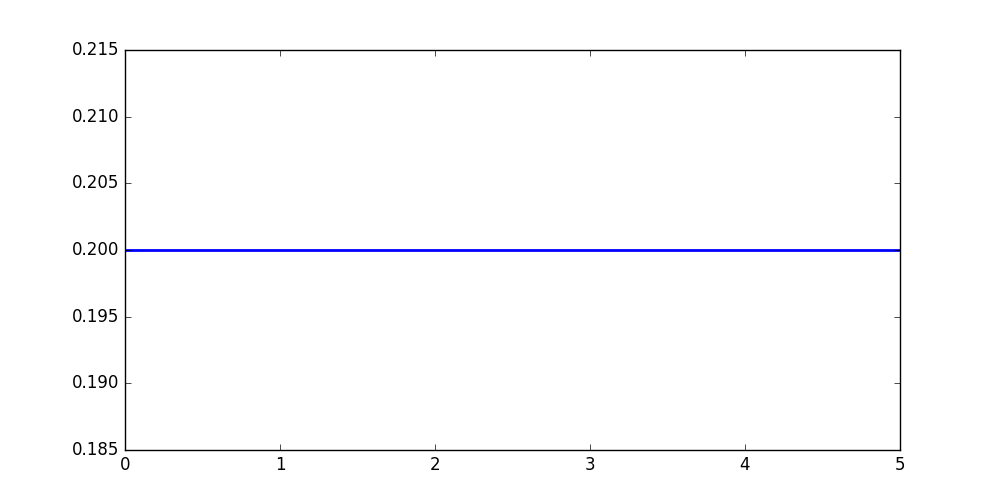
\includegraphics[width=\marginparwidth]{Pictures/uniform_0_5.png}}

\noindent This produces the picture in the margin. It describes the
probability density function (pdf) $f \colon [0,5] \rightarrow \RNpos$
with constant value $f(x) = \frac{1}{5}$, such that the integral
$\int_{0}^{5}f(x) \intd x$ equals $1$. The latter property is
essential for a probability distribution.\sidenote{A pdf $f\colon D
  \rightarrow \RNpos$ determines the probability of an event
  $U\subseteq D$ as the integral $\int_{U} f(x) \intd x$, with outcome
  in the unit interval $[0,1]$. It is the size of the surface under
  $f$ bounded by $U$. We shall describe this in probability in terms
  of validity later on.}

With the \EfProb libarary one can form joint distributions via
products \pythoninline{@}, also of discrete and continous
probabilities.
\begin{python}
>>> s = uniform_state(R(-1,1)) @ uniform_state(R(5,10))
>>> s
State on R(-1, 1) * R(5, 10)
>>> t = flip(0.3) @ s
>>> t
State on [True, False] * R(-1, 1) * R(5, 10)
\end{python}

\noindent We see that printing such states gives information about
their domains. Only 1-dimensional continuous states can be plotted.



\subsection{Operations on states}\label{subsec:cstate:operations}


\section{Predicates}\label{sec:cpred}


\subsection{Operations on predicates}\label{subsec:cpred:operations}


\subsection{Validity}\label{subsec:cpred:validity}


\subsection{Conditioning}\label{subsec:cpred:conditioning}


\section{Random variables}\label{sec:crandvar}




\section{Channels}\label{sec:cchannel}


\subsection{State transformation}\label{subsec:cchannel:statetransform}


\subsection{Structural channels}\label{subsec:cchannel:structural}





\chapter{Quantum Probability}\label{ch:qp}

The reader is assumed to be familiar with the basics of quantum
theory, see for instance\cite{NielsenC00,RieffelP11,YanofskyM08}.

\marginnote{To do: comparison with other quantum languages like
Quipper,\cite{GreenLRSV13} Qwire,\cite{PaykinRZ17}
LIQ$Ui\ket{}$,\cite{WeckerS14} and also to QuTiP.}

The code fragments shown in this chapter require the
\pythoninline{efprob_qu} library. It should be imported either on the
command line at the beginning of a session, or in the beginning of a
\Python file.

This chapter follows the same pattern as the previous two, discussing
states and predicates, random variables and channels, together with
many illustrations and some basic explanations of the underlying
mathematical structures. The quantum part of \EfProb is separate from
the (combined) discrete and continuous part. But discrete probability
does exist as special case within the \EfProb quantum world, as the
`diagonal' case in density matrices, see below. The operations on
states and predicates and channels are in general the same in quantum
probability as in the `classical' non-quantum probability, with
as notable exceptions:
\begin{itemize}
\item non-commutativity of certain operations, like sequential
conjunction $\andthen$ and conditioning of states;

\item non-copyability of states, because of the no-cloning property.
\end{itemize}


\section{States}\label{sec:qstate}

States in quantum theory are very different from states in discrete
probability and also from states in continuous
probability. Nevertheless, they do include discrete probabilistic
states as special case, as we shall see. Quantum states --- or simply
`states' in this chapter --- are represented as \emph{density
  matrices}.\index{density~matrix}\index{matrix!density~--} A state of
dimension $n$ is a represented as a matrix $\rho$ of dimension
$n\times n$, which is
positive\index{positive~matrix}\index{matrix!positive~--} and has
trace\index{trace} one: the elements on the diagonal add up to 
one. We sometimes use the standard notation $\Mat_n$ for the set of
arbitrary $n\times n$ (square) matrices over the complex numbers
$\CN$. Thus, a state of dimension $n$ is a special element
$\rho\in\Mat_n$, given by $n\times n$ complex numbers. Since it is
positive with trace $1$, all its elements on the diagonal are real
numbers, that add up to one.  Here we only consider finite-dimensional
states.

Let's see some examples, starting with dimension 2. States of this
dimension are called \emph{qubits}\index{qubit}. The two most familar
ones are written as \pythoninline{ket(0)}, \pythoninline{ket(1)},
\pythoninline{plus}, \pythoninline{minus} in:
\begin{python}
>>> ket(0)
[[ 1.  0.]
 [ 0.  0.]]
>>> ket(1)
[[ 0.  0.]
 [ 0.  1.]]
>>> plus
[[ 0.5+0.j  0.5+0.j]
 [ 0.5+0.j  0.5+0.j]]
>>> minus
[[ 0.5+0.j -0.5+0.j]
 [-0.5+0.j  0.5+0.j]]
\end{python}

\noindent The notation \pythoninline{0.j} is part of python's notation
for the imaginary part of complex numbers. In all of the above
examples the imaginary part is zero.\marginnote{The matrix of a state
  \pythoninline{s} can be accessed as \pythoninline{s.array}. It is
  what is (pretty) printed if you print a state.}

Please note that we deviate to some extend from standard quantum
notation where the ket notation $\ket{0}$ is used for the unit vector
$\left(\begin{smallmatrix} 1 \\ 0
\end{smallmatrix}\right) \in \CN^2$, and $\ket{1}$ for 
$\left(\begin{smallmatrix} 0 \\ 1 \end{smallmatrix}\right) \in \CN^2$.
Here \pythoninline{ket(0)} means the corresponding density matrix,
which is conventionally written as $\ket{0}\bra{0}$. Similarly,
\pythoninline{ket(1)} is $\ket{1}\bra{1}$. The two other states above,
\pythoninline{plus} and \pythoninline{minus}, are, respectively, the
density matrices:
$$\ket{+}\bra{+} 
\quad\mbox{and}\quad
\ket{-}\bra{-}
\quad\mbox{where}\quad
\left\{\begin{array}{rcl}
\ket{+}
& = &
\frac{1}{\sqrt{2}}(\ket{0} + \ket{1})
\\
\ket{-}
& = &
\frac{1}{\sqrt{2}}(\ket{0} - \ket{1})
\end{array}\right.$$

States can be defined `manually' as objects of the class
\pythoninline{State}. The constructor of this class takes an
array as argument, together with a domain. For instance, the 
states \pythoninline{ket(0)} and \pythoninline{ket(1)} could
be defined as:
\begin{python}
ket(0) = State(np.array([1,0], 
                        [0,0]]), [2])
ket(1) = State(np.array([0,0], 
                        [0,1]]), [2])
\end{python}

\noindent The Bell states\index{Bell!states} are pre-defined via outer
products as:
\begin{python}
bell00_vect = np.array([1,0,0,1])
bell01_vect = np.array([0,1,1,0])
bell10_vect = np.array([1,0,0,-1])
bell11_vect = np.array([0,1,-1,0])

bell00 = State(0.5 * np.outer(bell00_vect, bell00_vect), [2,2])
bell01 = State(0.5 * np.outer(bell01_vect, bell01_vect), [2,2])
bell10 = State(0.5 * np.outer(bell10_vect, bell10_vect), [2,2])
bell11 = State(0.5 * np.outer(bell11_vect, bell11_vect), [2,2])
\end{python}

\noindent Later in Subsection~\ref{subsec:qchannel:structural} we
shall see other ways to defined these states, namely via state
transformation. The same holds for the Greenberger-Horne-Zeilinger
(GHZ)\index{GHZ!states} states:
\begin{python}
ghz_vect1 = np.array([1,0,0,0,0,0,0,1])
ghz_vect2 = np.array([1,0,0,0,0,0,0,-1])
ghz_vect3 = np.array([0,0,0,1,1,0,0,0])
ghz_vect4 = np.array([0,0,0,1,-1,0,0,0])
ghz_vect5 = np.array([0,0,1,0,0,1,0,0])
ghz_vect6 = np.array([0,0,1,0,0,-1,0,0])
ghz_vect7 = np.array([0,1,0,0,0,0,1,0])
ghz_vect8 = np.array([0,1,0,0,0,0,-1,0])

ghz1 = State(0.5 * np.outer(ghz_vect1, ghz_vect1), [2,2,2])
ghz2 = State(0.5 * np.outer(ghz_vect2, ghz_vect2), [2,2,2])
ghz3 = State(0.5 * np.outer(ghz_vect3, ghz_vect3), [2,2,2])
ghz4 = State(0.5 * np.outer(ghz_vect4, ghz_vect4), [2,2,2])
ghz5 = State(0.5 * np.outer(ghz_vect5, ghz_vect5), [2,2,2])
ghz6 = State(0.5 * np.outer(ghz_vect6, ghz_vect6), [2,2,2])
ghz7 = State(0.5 * np.outer(ghz_vect7, ghz_vect7), [2,2,2])
ghz8 = State(0.5 * np.outer(ghz_vect8, ghz_vect8), [2,2,2])
\end{python}


\subsection{Operations on states}\label{subsec:qstate:operations}

This subsection describes the three operations that can be applied to
states themselves, namely \emph{parallel product}, \emph{convex sum},
and \emph{marginalisation}.  Later we shall see more operations that
produce new states, but they require other structures that we have not
yet described, like predicates for conditioning (see
Subsection~\ref{subsec:qpred:conditioning}) and channels for state
transformation (see Subsection~\ref{subsec:qchannel:statetransform}).

\paragraph{Product states} As before we can form 
product
states\index{product!of~quantum~states}\index{state!quantum~product~--}
--- also called joint states --- by putting states in parallel via the
binary operator \pythoninline{@}.
\begin{python}
>>> ket(0) @ ket(1)
[[ 0.  0.  0.  0.]
 [ 0.  1.  0.  0.]
 [ 0.  0.  0.  0.]
 [ 0.  0.  0.  0.]]
>>> ket(1) @ plus
[[ 0.0+0.j  0.0+0.j  0.0+0.j  0.0+0.j]
 [ 0.0+0.j  0.0+0.j  0.0+0.j  0.0+0.j]
 [ 0.0+0.j  0.0+0.j  0.5+0.j  0.5+0.j]
 [ 0.0+0.j  0.0+0.j  0.5+0.j  0.5+0.j]]
\end{python}

\noindent The resulting matrix is the \emph{Kronecker
  product}\index{Kronecker!product}\index{product!Kronecker~--} of the
two matrices. As one sees, the size of these matrices grows
quickly. Indeed, the product of an $n$-dimensional state and an
$m$-dimensional state has dimension $n\times
m$.\sidenote{\label{note:qstate:type}We have said that a qubit has
  dimension $2$. Each state \pythoninline{s} has a domain attribute
  called \pythoninline{s.dom}. It returns a list of dimensions of all
  its component states. For instance for the large example state we
  can ask for \pythoninline{((plus @ ket(0)) ** 4).dom} and get
  \pythoninline{[2, 2, 2, 2, 2, 2, 2, 2]}. This domain is used as the
  \emph{type} of a state, and is checked when states are combined with
  for instance predicates or channels. The size
  \pythoninline{s.dom.size} is the product of all numbers in
  \pythoninline{dom}.}


There is a short-hand \pythoninline{ket(0,0)} for the product
\pythoninline{ket(0) @ ket(0)}. An arbitrary tuple of
\pythoninline{0}'s and \pythoninline{1}'s can be used as input to the
function \pythoninline{ket}:
\begin{python}
>>> ket(0,1,1)
[[ 0.  0.  0.  0.  0.  0.  0.  0.]
 [ 0.  0.  0.  0.  0.  0.  0.  0.]
 [ 0.  0.  0.  0.  0.  0.  0.  0.]
 [ 0.  0.  0.  1.  0.  0.  0.  0.]
 [ 0.  0.  0.  0.  0.  0.  0.  0.]
 [ 0.  0.  0.  0.  0.  0.  0.  0.]
 [ 0.  0.  0.  0.  0.  0.  0.  0.]
 [ 0.  0.  0.  0.  0.  0.  0.  0.]]
\end{python}

\noindent This is the same as \pythoninline{ket(0) @ ket(1) @ ket(1)}.
Using other entries than \pythoninline{0} or \pythoninline{1} yields
an exception.

Products can also be iterated as:
\begin{python}
>>> ket(0) ** 3
[[ 1.  0.  0.  0.  0.  0.  0.  0.]
 [ 0.  0.  0.  0.  0.  0.  0.  0.]
 [ 0.  0.  0.  0.  0.  0.  0.  0.]
 [ 0.  0.  0.  0.  0.  0.  0.  0.]
 [ 0.  0.  0.  0.  0.  0.  0.  0.]
 [ 0.  0.  0.  0.  0.  0.  0.  0.]
 [ 0.  0.  0.  0.  0.  0.  0.  0.]
 [ 0.  0.  0.  0.  0.  0.  0.  0.]]
\end{python}

\noindent This is \pythoninline{ket(0) @ ket(0) @ ket(0)}, which is
the same as \pythoninline{ket(0,0,0)}. The operators \pythoninline{@}
and \pythoninline{**} can be combined, leading quickly to large states
like:\sidenote{The parallel product operator \pythoninline{@} is
  `strictly' associative, so that \pythoninline{(s1 @ s2) @ s3} and
  \pythoninline{s1 @ (s2 @ s3)} are the same states.}
\begin{python}
>>> (plus @ ket(0)) ** 4
>>> ...
\end{python}


\paragraph{Convex sums of states} The second construction on states in this 
subsection is the convex sum.\index{convex!sum~of~quantum~states} It
involves a weighted sum of states where the weights add up to one, as
in:
\begin{python}
>>> convex_state_sum((0.2,ket(0)),(0.3,plus),(0.5,minus))
[[ 0.6+0.j -0.1+0.j]
 [-0.1+0.j  0.4+0.j]]
\end{python}

%% \noindent For binary convex sums one can also use the following syntax:
%% \begin{python}
%% >>> (ket(0) + ket(1))(0.2)
%% [[ 0.2  0. ]
%%  [ 0.   0.8]]
%% \end{python}

%% \noindent This is the same as \pythoninline{convex_state_sum((0.2,
%%   ket(0)), (0.8, ket(1)))}

\paragraph{Marginalisation} Via products one joins states together.
Marginalisation is the reverse operation that deletes certain parts
of joint product states. How this works is best illustrated via
an example:
\begin{python}
>>> ket(0) @ ket(1) @ plus @ minus % [1,0,1,0]
[[ 0.5+0.j  0.5+0.j  0.0+0.j  0.0+0.j]
 [ 0.5+0.j  0.5+0.j  0.0+0.j  0.0+0.j]
 [ 0.0+0.j  0.0+0.j  0.0+0.j  0.0+0.j]
 [ 0.0+0.j  0.0+0.j  0.0+0.j  0.0+0.j]]
\end{python}

\noindent The post-fix selection operation \pythoninline{\%[1,0,1,0]}
selects the first and third component --- indicated by
\pythoninline{1} in first and third position in the selector
\pythoninline{[1,0,1,0]} --- from the joint state, and removes the
second and fourth component --- indicated by \pythoninline{0} in the
second and fourth position. What remains in the example is the product
state \pythoninline{ket(0) @ plus}. Mathematically this
marginalisation operation takes the appropriate partial
traces.\sidenote{We have described in
  sidenote~\getrefnumber{note:qstate:type} that the domain attribute
  `dom' of a state is a list of dimensions of the components states,
  say \pythoninline{[2,2,4]}, and that such lists are used as types
  for states. A selector in marginalisation must match such dom
  attribute, and in this case also be of length three, consisting of
  \pythoninline{0}'s and \pythoninline{1}'s, describing whether each
  of these components must be kept or removed. If a marginalisation
  selector does not match the type of a state, an exception is
  raised.}

Marginalisation exists in a quantum setting because quantum
bits/information can be discarded. But since there is no
\emph{cloning} in a quantum world, there is no copy operation.  As
already mentioned in the beginning of this chapter, this is a crucial
difference with the world of classical (discrete and continuous)
probability.

In general, a joint state \pythoninline{s} is different from the
product of its marginals, that is, \pythoninline{s} is not equal to
\pythoninline{(s \% [1,0]) @ (s \% [0,1])}. This is due to possible
\emph{entanglement}\index{entanglement} within \pythoninline{s}.  Via
such entanglement one part of the state can influence the other part,
as we have also seen in classical probability theory, see
Example~\ref{ex:diseasemood}. But quantum entanglement is stronger
than probabilistic entwinedness.





\subsection{Basic states}\label{subsec:qstate:basic}

We have already seen basic states like \pythoninline{ket(0)},
\pythoninline{ket(1)}, \pythoninline{plus}, \pythoninline{minus}.
This section describes several more functions that produce quantum
states, namely:
\begin{itemize}
\item probabilistic states

\item vector states

\item random states
\end{itemize}

\paragraph{Probabilistic states}

A quantum state is called \emph{probabilistic} if its all its non-zero
matrix entries are on the diagonal. These entries are then necessarily
real and add up to one. The states \pythoninline{ket(0)} and
\pythoninline{ket(1)} are thus probabilistic, but \pythoninline{plus}
and \pythoninline{minus} are not. Probabilistic states are often
called \emph{classical} states.

There is function that takes an arbitrary-length tuple of numbers,
normalises them, and turns them into a probabilistic state:
\begin{python}
>>> probabilistic_state(3,4,1)
[[ 0.375  0.     0.   ]
 [ 0.     0.5    0.   ]
 [ 0.     0.     0.125]]
\end{python}

\noindent There is a special function for the binary case:
\begin{python}
>>> cflip(0.3)
[[ 0.3  0. ]
 [ 0.   0.7]]
\end{python}

\noindent where \pythoninline{cflip} stand for `classical flip'.  It
yields the same outcome as \pythoninline{probabilistic_state(0.3,
  0.7)} and as \pythoninline{probabilistic_state(3, 7)}. There are
further abbreviations \pythoninline{cfflip} for
\pythoninline{cflip(0.5)}, giving a classical `fair' flip. These are
just different names for \pythoninline{ket(0)} and
\pythoninline{ket(1)}.

The product and convex sum of probabilistic states is again
probabilistic. For instance:
\begin{python}
>>> cfflip @ probabilistic_state(2,2,1)
[[ 0.2  0.   0.   0.   0.   0. ]
 [ 0.   0.2  0.   0.   0.   0. ]
 [ 0.   0.   0.1  0.   0.   0. ]
 [ 0.   0.   0.   0.2  0.   0. ]
 [ 0.   0.   0.   0.   0.2  0. ]
 [ 0.   0.   0.   0.   0.   0.1]]
\end{python}


\paragraph{Vector states} Each vector $\ket{v}$ of norm $1$ yields
a state / density matrix $\ket{v}\bra{v}$, which is often called a
vector state.\index{state!vector~--}\index{vector~state} Thus, by
provinding an $n$-tuple of complex numbers we can get a
state. Implicitly, the numbers are normalised:
\begin{python}
>>> vector_state(1, complex(1, 2), -2)
[[ 0.1+0.j   0.1-0.2j -0.2-0.j ]
 [ 0.1+0.2j  0.5+0.j  -0.2-0.4j]
 [-0.2+0.j  -0.2+0.4j  0.4+0.j ]]
\end{python}


In the 2-dimensional case such a vector $\ket{v}$ is of
the form $\ket{v} = \left(\begin{smallmatrix} \alpha \\ \beta
\end{smallmatrix}\right)$, where $\alpha,\beta\in\CN$ are complex numbers
with $|\alpha|^{2} + |\beta|^{2} = 1$. The resulting density matrix
is:
$$\left(\begin{array}{ccc}
|\alpha|^{2} & & \alpha\cdot\overline{\beta}
\\
\overline{\alpha}\cdot \beta & & |\beta|^{2}
\end{array}\right)$$

\begin{python}
>>> vector_state(0.5 * sqrt(3), complex(0, 0.5))
[[ 0.75+0.j         0.00-0.4330127j]
 [ 0.00+0.4330127j  0.25+0.j       ]]
\end{python}

There is a general result saying that each (finite-dimensional)
density matrix can be written as a convex combination (a `mixture') of
`pure' vector states, via spectral decomposition, see
\eg~Thm.~2.5 of\cite{NielsenC00}.

A \emph{unit state}\index{state!quantum~unit~--} is a special case of
a vector state --- and also of a probabilistic state. It puts a single
\pythoninline{1} at the indicated position of the diagonal:
\begin{python}
>>> point_state(2,3)
[[ 0.  0.  0.]
 [ 0.  0.  0.]
 [ 0.  0.  1.]]
\end{python}

\noindent This is the same as \pythoninline{vector\_state(0,0,1)}.


\paragraph{Random states} For testing purposes it is very useful
to have randomly generated states of a certain length. For instance:
\begin{python}
>>> random_state(3)
[[ 0.32162863+0.j          0.23537749-0.07970437j -0.08834685-0.11437522j]
 [ 0.23537749+0.07970437j  0.49432253+0.j         -0.08974455+0.06699254j]
 [-0.08834685+0.11437522j -0.08974455-0.06699254j  0.18404884+0.j        ]]
\end{python}

\noindent Each time this function is called a new random state is
produced, using the underlying random number generator of python.

There is a similar function that produces a random probabilistic state,
as in:
\begin{python}
>>> random_probabilistic_state(2)
[[ 0.59979369  0.        ]
 [ 0.          0.40020631]]
\end{python}

\noindent Earlier, in the beginning of Section~\ref{sec:qstate}, we
already described the Bell and GHZ states, essentially as vector
states.



\section{Predicates}\label{sec:qpred}

The distinction between states and predicates is fundamental in our
approach to probability theory, both in the classical and in the
quantum case. Having seen quantum states, we now introduce quantum
predicates. In combination with states we can obtain the
\emph{validity} of a predicate in a state, and also the state
\emph{conditioned} by a predicate. But first we shall describe
predicates on their own, with several ways to combine them into new
predicates.

Mathematically, a predicate $p$ of dimension $n$ is an $n\times n$
matrix $p\in\Mat_n$ over the complex numbers, which is positive and
below the identity: $0 \leq p \leq 1$, there $0, 1 \in \Mat_{n}$ are
the zero matrix and the identity matrix respectively. These quantum
predicates are often called \emph{effects}.\index{effect} A predicate
$p$ is called
\emph{sharp}\index{sharp~predicate!quantum~--}\index{predicate!sharp~quantum~--}
if $p\cdot p = p$.  The matrices of predicates may involve complex
numbers, as for instance in:
$$\frac{1}{2}\left(\begin{array}{ccc}
1 & & -i
\\
i & & 1
\end{array}\right)$$

If $\omega\in\Mat_n$ is a state and $p\in\Mat_n$ is a predicate, then
the validity $\omega\models p$ of $p$ in $\omega$ is defined as the
number in the unit interval $[0,1]$ defined as:
\begin{equation}
\label{eqn:qvalidity}
\begin{array}{rcl}
\omega\models p
\;=\;
\tr(\omega\cdot p),
\end{array}
\end{equation}

\noindent where $\tr$ is the trace operation and $\cdot$ is matrix
composition. This equation is also known as Born's rule.

The most basic predicates are truth and falsity:
\begin{python}
>>> falsity(2)
[[ 0.  0.]
 [ 0.  0.]]
>>> truth(2,3)
[[ 1.  0.  0.  0.  0.  0.]
 [ 0.  1.  0.  0.  0.  0.]
 [ 0.  0.  1.  0.  0.  0.]
 [ 0.  0.  0.  1.  0.  0.]
 [ 0.  0.  0.  0.  1.  0.]
 [ 0.  0.  0.  0.  0.  1.]]
\end{python}

\noindent Notice that the arguments of \pythoninline{falsity} and
\pythoninline{truth} are not single dimensions but lists of
dimensions. These domains describe the type of a state, see
sidenote~\getrefnumber{note:qstate:type}, and make it possible to
define truth and falsity on an entire product state at once, by using
the appropriate domain of the product state as input. Thus, the
predicate \pythoninline{truth(2,3)} used above is the same
as the parallel product \pythoninline{truth(2) @ truth(3)} that
will be described below.

A \emph{probabilistic} predicate has, like a probabilistic state, only
real entries from $[0,1]$ on its diagonal, but these entries need not
add up to one. There is a function that produces such a probabilistic
predicate of dimension $n$ from an $n$-tuple of numbers in the unit
interval.
\begin{python}
>>> probabilistic_pred(0.1,1,0.25,0.0)
[[ 0.1   0.    0.    0.  ]
 [ 0.    1.    0.    0.  ]
 [ 0.    0.    0.25  0.  ]
 [ 0.    0.    0.    0.  ]]
\end{python}

\noindent As a special case there are `unit' predicates that put a
\pythoninline{1} at the given position of the diagonal:
\begin{python}
>>> point_pred(2,4)
[[0 0 0 0]
 [0 0 0 0]
 [0 0 1 0]
 [0 0 0 0]]
\end{python}

For testing purposes one can use
\pythoninline{random_pred(n)} and
\pythoninline{random_probabilistic_pred(n)} to get
arbitrary (probabilist) predicates of dimension \pythoninline{n}.

Each state of dimension $n$ is also a predicate of dimension $n$, but
not the around --- take \pythoninline{falsity} for instance. There is
a way in \EfProb to turn a state into a predicate, via the method
\pythoninline{as\_pred()}, but it will not be used frequently.  Since
the distinction between predicates and states is so fundamental, we
prefer to define predicates immediately as predicates, and not first
as states. For this reason there is a function
\pythoninline{vector\_pred}, in analogy with
\pythoninline{state\_pred}.  It turns a vector $\ket{v}$ into the
outer product $\ket{v}\bra{v}$, considered as a predicate.

Again, it is important not to confuse states and predicates.  They are
very different. As we shall see next, there are several logical
operations on predicates which do not exists for states, in the sense
that states are not closed under these operations.



\subsection{Operations on predicates}\label{subsec:qpred:operations}

We shall discuss the following operations on predicates.
\begin{itemize}
\item orthosupplement, or negation \pythoninline{\~}

\item scalar multiplication \pythoninline{*}

\item partial sum \pythoninline{+}

\item parallel conjunction \pythoninline{@}

\item sequential conjunction \pythoninline{\&}

\item weakening.
\end{itemize}

\noindent The first three points capture the \emph{effect module}
structure of quantum predicates. This effect module structure is
common for predicates in discrete, continuous, and quantum
probability.


\paragraph{Orthosupplement} Negation in a probabilistic or quantum
setting is called orthosupplement.\index{orthosupplement!quantum~--}
Here it is written as $\ortho p$, but in the literature one often sees
$p^{\bot}$ instead. On the unit interval $[0,1]$ orthosupplement is
given by $\ortho r = 1 - r$. In a quantum setting the orthosupplement
of a predicate is given similarly, by subtracting the predicate from
the identity (diagonal) matrix. Thus, $\ortho p = 1 - p$, see:
\begin{python}
>>> p = random_pred(2)
>>> p
[[ 0.36250803+0.j         -0.15404606-0.00875401j]
 [-0.15404606+0.00875401j  0.96265550+0.j        ]]
>>> ~p
[[ 0.63749197+0.j          0.15404606+0.00875401j]
 [ 0.15404606-0.00875401j  0.03734450+0.j        ]]
\end{python}

\noindent Notice that the orthosupplement of a probabilistic predicate
is probabilistic again. Obviously, taking the orthosupplement twice
returns the original predicate. Hence the `double negation' rule of
classical (Boolean) logic holds. But the logic of
quantum/probabilistic predicate is not Boolean. Its structure is
captured algebraically in terms of effect modules.


\paragraph{Scalar multiplication} Predicates are closed under
multiplication\index{scalar~multiplication!quantum~--} with a scalar
from the unit interval $[0,1]$.  Each element of the matrix is then
multiplied by the scalar.  Here is a simple probabilistic example.
\begin{python}
>>> 0.3 * probabilistic_pred(0.2,0.5)
[[ 0.06  0.  ]
 [ 0.    0.15]]
\end{python}

\noindent Probabilistic predicates are closed under scalar
multiplication, but sharp predicates are not.


\paragraph{Partial sum} Addition of numbers $r,s\in [0,1]$ in
the unit interval is a partial operation, which is defined only if
$r+s\leq 1$. This sum is commutative and associative in a suitable
partial sense. Similarly there is a partial
sum\index{partial~sum!of~quantum~predicates} of predicates, which is
given by (elementwise) sum of matrices, as long as the resulting
matrix is still below the identity (matrix). Here is an example.
\begin{python}
>>> point_pred(2,4) + point_pred(0,4)
[[1 0 0 0]
 [0 0 0 0]
 [0 0 1 0]
 [0 0 0 0]]
\end{python}

\noindent It is not hard to see that a convex sum of predicates always
exists. Such sums can be written simply as \pythoninline{0.3 * p1 +
  0.6 * p2 + 0.1 * p3} for predicates \pythoninline{p1, p2, p3}.  This
works in the same way for $n$-ary convex sums, for any fixed $n\geq
1$.

A \emph{test}\index{test} is a finite list of predicates
\pythoninline{p1}, \ldots, \pythoninline{pn}, all with the same
domain, whose sum \pythoninline{p1 + ... + pn} equals truth.  Such
tests are used in measurements, see
Subsection~\ref{subsec:qchannel:measurement}. The bell and GHZ basis
vectors mentiond at the end of Section~\ref{sec:qstate} give rise to
the following Bell\index{Bell!test} and GHZ\index{GHZ!test} tests,
in which these states are used as predicates.
\begin{python}
>>> bell_test = [bell00.as_pred(), bell01.as_pred(), 
...              bell10.as_pred(), bell11.as_pred()]
>>> ghz_test = [ghz1.as_pred(), ghz2.as_pred(), 
...             ghz3.as_pred(), ghz4.as_pred(), 
...             ghz5.as_pred(), ghz6.as_pred(), 
...             ghz7.as_pred(), ghz8.as_pred()]
\end{python}

\noindent Indeed, the Bell predicates form a test (and the GHZ
predicates too):
\begin{python}
>>> bell00.as_pred() + bell01.as_pred() + bell10.as_pred() + bell11.as_pred()
[[ 1.  0.  0.  0.]
 [ 0.  1.  0.  0.]
 [ 0.  0.  1.  0.]
 [ 0.  0.  0.  1.]]
\end{python}

\noindent When the matrix sum $p+q$ of two predicates $p,q$ is not
below the identity, their sum still exists in \EfProb, but it no
longer a predicate. It has become a random variable, see
Section~\ref{sec:qrandvar} for details.



\paragraph{Parallel conjunction} If \pythoninline{p1} is a predicate
on state \pythoninline{s1} and \pythoninline{p2} is a predicate on
\pythoninline{s2}, then there is a parallel
conjunction\index{parallel~conjunction!of~quantum~predicates}
predicate \pythoninline{p1 @ p2} on the product state \pythoninline{s1
  @ s2}.  It is obtained via the Kronecker
product\index{Kronecker!product}\index{product!Kronecker~--} of the
two matrices, just like for states. The predicate \pythoninline{p1 @
  p2} is like a multiplication, see \eg in:
\begin{python}
>>> truth(2) @ falsity(3)
[[ 0.  0.  0.  0.  0.  0.]
 [ 0.  0.  0.  0.  0.  0.]
 [ 0.  0.  0.  0.  0.  0.]
 [ 0.  0.  0.  0.  0.  0.]
 [ 0.  0.  0.  0.  0.  0.]
 [ 0.  0.  0.  0.  0.  0.]]
\end{python}

\noindent In this way the underlying matrices grow considerable in
size.\sidenote[][-3\baselineskip]{\label{note:qpred:type}When we take
  the sum \pythoninline{p+q} of two predicates, these predicates
  \pythoninline{p} and \pythoninline{q} have to have \emph{the same
    domain}. This domain of a predicate is the same as the domain of a
  state, as sketched in sidenote~\ref{note:qstate:type}: it is given
  by a list of natural numbers describing the dimensions of their
  components.  These dimension lists (domains) are simply concatenated
  in the operation \pythoninline{@}, both for states and for
  predicates. We often informally say things like ``\pythoninline{p}
  is a predicate on states \pythoninline{s}''. This means that
  \pythoninline{p} and \pythoninline{s} have the same domain/type, as
  given by their \pythoninline{dom} attribute. }


\paragraph{Sequential conjunction} For two predicates \pythoninline{p},
\pythoninline{q} of the same type, there is a predicate
\pythoninline{p \& q} for sequential
conjunction.\index{sequential~conjunction!of~quantum~predicates} It is
pronounced as `\pythoninline{p} and-then \pythoninline{q}'. The order
is relevant, since this conjunction \pythoninline{\&} is \emph{not}
commutative in the quantum case --- unlike in classical probability.

The mathematical interpretation of `and-then' is given by:
\begin{equation}
\label{eqn:qandthen}
\begin{array}{rcl}
p \andthen q
& = &
\sqrt{p} \cdot q \cdot \sqrt{p}.
\end{array}
\end{equation}

\noindent Here we use $\sqrt{p}$ as the square root of the
\emph{matrix} \pythoninline{p}.\sidenote{The square root of a matrix
  is not the same thing as the square root of its elements
  separately. The standard way to obtain the square root of a positive
  (\ie non-negative, sometimes called positive definite) matrix $M$ is
  to diagonalise $M$ as $M = VEV^*$, where $E$ is a diagonal matrix
  containing the (positive) eigenvalues of $M$. Let $D$ be the
  diagonal matrix with the square roots of the eigenvalues in $E$,
  taken elementwise. Then $\sqrt{M} = VDV^{*}$.} It exists since $p$,
as a predicate, is positive. This construction is sometimes called
\emph{L\"uders rule}.\index{L\"uders~rule} It's role will be
illustrated in Example~\ref{ex:polarisation}. Here we just use a
probabilistic example, where sequential conjunction \pythoninline{\&}
is simply pointwise multiplication --- and thus commutative.
\begin{python}
>>> probabilistic_pred(0.2,0.8) & probabilistic_pred(0.4, 0.6)
[[ 0.08  0.  ]
 [ 0.    0.48]]
\end{python}

\noindent We shall see illustrations of non-commutativity of $\andthen$
later on, for instance in Example~\ref{ex:polarisation}.


\paragraph{Weakening}
Weakening\index{weakening!of~quantum~predicates} is a structural rule
in logic that makes it possible to ``widen the context'', see the
general explanation at the end of
Subsection~\ref{subsec:dpred:validity} for discrete probability. It
works the same way in quantum probability: we have to deal with
weakening explicitly, namely via parallel conjunction with truth:
\begin{python}
>>> t = ket(0,0)
>>> p = point_pred(1,2)
>>> s >= p
0.6
>>> s @ t >= p @ truth(2,2)
0.6
\end{python}

%% \noindent Weakening thus involves some burocracy. One has to be
%% careful to provide the truth predicate with the appropriate
%% domain. One way of doing this is simply by extracting it form the
%% additional state components, as in:\sidenote{The \pythoninline{*} is
%%   needed in \pythoninline{truth(*t.dom.dims)} since the argument of
%%   \pythoninline{truth} is a list, which has to be converted into a
%%   tuple by \Python.}
%% \begin{python}
%% >>> t @ s @ t >= truth(*t.dom.dims) @ p @ truth(*t.dom.dims)
%% 0.6
%% \end{python}



\subsection{Validity}\label{subsec:qpred:validity}

As we already mentioned in the beginning of Section~\ref{sec:qpred},
validity\index{validity!quantum~--} $\omega\models p$ of a predicate
$p$ in a state $\omega$ is a very basic notion. In \Python the
operator that is most similar to `$\models$' is
\pythoninline{>=}. Hence this what we shall use.
Equation~\eqref{eqn:qvalidity} describes $\omega\models p$ as the
trace $\tr(\omega\cdot p)$ of the product. It can be understood as the
Hilbert-Schmidt inner product $\tuple{\omega\mid p}$, using that $p^*
= p$.
\begin{python}
>>> v = vector_pred(0.5 * sqrt(3), complex(0, 0.5))
>>> v
[[ 0.75+0.j         0.00-0.4330127j]
 [ 0.00+0.4330127j  0.25+0.j       ]]
>>> ket(0) >= v
0.75
>>> ket(1) >= v
0.25
\end{python}

Validity $\models$ satisfies some basic mathematical properties:
$$\begin{array}{rcl}
\omega \models \truth
& = &
1
\\
\omega \models \falsity
& = &
0
\\
\omega\models \ortho p
& = &
1 - (\omega\models p)
\\
\omega \models r * p
& = &
r * (\omega\models p)
\\
\omega \models p_{1} + p_{2}
& = &
(\omega\models p_{1}) + (\omega\models p_{2})
\\
\omega \tensor \sigma \models p \tensor q
& = &
(\omega\models p) \cdot (\sigma\models q).
\end{array}$$

\noindent Such properties can be tested (but not proven!) by using
random states and predicates, as in:
\begin{python}
>>> s = random_state(100)
>>> p = random_pred(100)
>>> s >= 0.3 * p
0.05918743186783347
>>> 0.3 * (s >= p)
0.059187431867833463
\end{python}

\noindent Using validity we can now easily see that sequential
conjunction $\andthen$ is \emph{not commutative}:
\begin{python}
>>> p = point_pred(0,2)
>>> q = plus.as_pred()
>>> ket(0) >= p & q
0.5
>>> ket(0) >= q & p
0.25
\end{python}

\noindent See Example~\ref{ex:polarisation} for more such examples.

Since a state can be turned into a predicate, we can write states on
both sides of the validity operator \pythoninline{>=}, where we do need
to turn the state on the right hand side into a predicate. The resulting
validity does not depend on which of the two states is used as
predicate.
\begin{python}
>>> s = random_state(8)
>>> t = random_state(8)
>>> s >= t.as_pred()
0.116791838672 
>>> t >= s.as_pred()
0.116791838672
\end{python}

\noindent If these states \pythoninline{s} and \pythoninline{t} are
vector states, then validity corresponds to the square of the inner product
of the underlying states, as tested in:
\begin{python}
>>> v1 = np.random.rand(5)
>>> v2 = v1/np.linalg.norm(v1)
>>> w1 = np.random.rand(5)
>>> w2 = w1/np.linalg.norm(w1)
>>> s = vector_state(*v2)
>>> t = vector_state(*w2)
>>> s >= t.as_pred()
0.659104940735
>>> np.inner(v2, w2) ** 2 
0.659104940735
\end{python}


\auxproof{
\begin{example}
\label{ex:linda}
We illustrate sequential conjunction \pythoninline{\&} and disjunction
\pythoninline{|} in the famous \emph{Linda
  problem}\index{Linda~problem} leading to `conjunction
fallacies'\index{conjunction!fallacy}\index{fallacy!conjunction~--}
and `disjunction
falacies',\index{disjunction!fallacy}\index{fallacy!disjunction~--}
with their explanation in quantum cognition.\index{quantum~cognition}
We follow the description in\cite{BusemeyerB12}. Consider the
following quote and subsequent questions.
\begin{quote}
Linda is 31 years old, single, outspoken and very bright. She majored
in philosophy. As a student, she was deeply concerned with issues of
discrimination and social justice, and also participated in
anti-nuclear demonstrations.
\end{quote}

\noindent What is the likelihood of the following events? Linda is:
\begin{enumerate}
\item \label{ex:linda:fem} active in the feminist movement;
\item \label{ex:linda:bank} a bank teller;
\item \label{ex:linda:femandbank} active in the feminist movement and a
  bank teller;
\item \label{ex:linda:femorbank} active in the feminist movement or a
  bank teller.
\end{enumerate}

\noindent The `conjunction fallacy' concerns the fact that when asked
many people say that option~\eqref{ex:linda:femandbank} is more likely
than option~\eqref{ex:linda:bank}, and the `disjunction fallacy'
occurs when option~\eqref{ex:linda:fem} is judged to be more likely
than option~\eqref{ex:linda:femorbank}.

We illustrate how to realise these fallacies using the
following state from\cite{BusemeyerB12}.
\begin{python}
>>> s = vector_state(0.987, -0.1564)
>>> feminist = point_pred(0,2)
>>> bankteller = vector_pred(cos(0.4 * pi), sin(0.4 * pi))
>>> s >= feminist 
0.97550548153
>>> s >= bankteller 
0.0244489755636
>>> s >= feminist & bankteller
0.0931524844331
>>> s >= bankteller | feminist
0.906843166606
\end{python}

\noindent In this example the probability that Linda is \emph{both} a
feminist and a bankteller (option~\ref{ex:linda:femandbank}) is higher
than the probability that she is only a bankteller
(option~\ref{ex:linda:bank}). Similarly, the probability that Linda is
a bankteller \emph{or} a feminist (option~\ref{ex:linda:femorbank}) is
lower than the probability that she is just a feminist
(option~\ref{ex:linda:fem}).

The above probabilities coincide with the numbers
in\cite{BusemeyerB12}.  There is an important difference however: here
these probabilities are obtained in an intuitive, high-level manner,
via validities of generally defined `and' and `or' formulas in the
logic of effects. In \emph{loc.\ cit.} they arise from detailed
low-level calculations via inner products in the Hilbert space
$\CN^2$. All that complexity is hidden here.  Similar illustrations
are given in Examples~\ref{ex:carpreference} and~\ref{??}.
\end{example}

    print("* Linda example")
    s = vector_state(0.987, -0.1564)
    feminist = point_pred(0,2)
    bankteller = vector_pred(cos(0.4 * pi), sin(0.4 * pi))
    print( s >= feminist )
    print( s >= bankteller )
    print( s >= feminist & bankteller )
    print( s >= bankteller | feminist )

    print("\n===\n")

}


\begin{example}
\label{ex:belltable}
The Bell states are famous 2-qubit states which have been defined at
the end of Section~\ref{sec:qstate}. Of these four states be use the
one named \pythoninline{bell00}. We additionally use the following
predicates, obtained from states.
\begin{python}
>>> A1 = vector_pred(1/sqrt(2), 1/sqrt(2))
>>> B1 = A1
>>> A2 = vector_pred(1/sqrt(2), 0.5/sqrt(2) * complex(1, sqrt(3)))
>>> B2 = A2
>>> A1
[[ 0.5  0.5]
 [ 0.5  0.5]]
>>> A2
[[ 0.50+0.j         0.25-0.4330127j]
 [ 0.25+0.4330127j  0.50+0.j       ]]
\end{python}

\noindent These predicates may look a bit \emph{ad hoc} at this
stage,\sidenote[][-1\baselineskip]{\label{sidenote:abramskycalculations}Detailed
  calculations and explanations of the coice of these predicates can
  be found at \url{https://arxiv.org/abs/1406.7386}.} but later in
Subsection~\ref{subsec:qchannel:predtransform} we show how they can be
described in a more systematic manner via predicate transformation.

The valdities of the parallel conjunctions of the predicates
\pythoninline{A1}, \pythoninline{A2}, \pythoninline{B1},
\pythoninline{B2} and their orthosupplements yield the famous
Bell-tables\index{Bell!table} that play an important role in
non-locality\index{non-locality} in quantum foundations, see
\eg\cite{AbramskyB11} for more information. The table below summarises
the validities of the 4-tuples of predicates, forming a test:
$$\mbox{\pythoninline{Ai @ Bj, Ai @ ~Bj, ~Ai @ Bj, ~Ai @ ~Bj}}$$

\noindent for $i,j \in \{1,2\}$.

\bigskip

\begin{fullwidth}
\begin{center}
\begin{tabular}{c|c|c|c}
{\pythoninline{bell00 >= A1 @ B1}} &
   {\pythoninline{bell00 >= A1 @ ~B1}} &
   {\pythoninline{bell00 >= ~A1 @ B1}} &
   {\pythoninline{bell00 >= ~A1 @ ~B1}}
\\
\hline
\hline
0.5 & -1.11022302463e-16 & -1.11022302463e-16 & 0.5
\\
\hline
& & & \\
%% \end{tabular}
%% \end{center}
%% \end{fullwidth}

%% \smallskip

%% \noindent Using the predicate \pythoninline{B2} instead of
%% \pythoninline{B1} yields:

%% \smallskip

%% \begin{fullwidth}
%% \begin{center}
%% \begin{tabular}{c|c|c|c}
{\pythoninline{bell00 >= A1 @ B2}} &
   {\pythoninline{bell00 >= A1 @ ~B2}} &
   {\pythoninline{bell00 >= ~A1 @ B2}} &
   {\pythoninline{bell00 >= ~A1 @ ~B2}}
\\
\hline
\hline
0.375 & 0.125 & 0.125 & 0.375
\\
\hline
& & & \\
%% \end{tabular}
%% \end{center}
%% \end{fullwidth}

%% \smallskip

%% \noindent By changing \pythoninline{A1} into \pythoninline{A2} one
%% gets:

%% \smallskip

%% \begin{fullwidth}
%% \begin{center}
%% \begin{tabular}{c|c|c|c}
{\pythoninline{bell00 >= A2 @ B1}} &
   {\pythoninline{bell00 >= A2 @ ~B1}} &
   {\pythoninline{bell00 >= ~A2 @ B1}} &
   {\pythoninline{bell00 >= ~A2 @ ~B1}}
\\
\hline
\hline
0.375 & 0.125 & 0.125 & 0.375
\\
\hline
& & & \\
%% \end{tabular}
%% \end{center}
%% \end{fullwidth}

%% \smallskip

%% \noindent Finally:
%% \begin{fullwidth}
%% \begin{center}
%% \begin{tabular}{c|c|c|c}
{\pythoninline{bell00 >= A2 @ B2}} &
   {\pythoninline{bell00 >= A2 @ ~B2}} &
   {\pythoninline{bell00 >= ~A2 @ B2}} &
   {\pythoninline{bell00 >= ~A2 @ ~B2}}
\\
\hline
\hline
0.125 & 0.375 & 0.375 & 0.125
\end{tabular}
\end{center}
\end{fullwidth}
\end{example}


\subsection{Conditioning}\label{subsec:qpred:conditioning}

Validity $\omega\models p$ is one way to combine states and
predicates. When this validity is non-zero, one can also form the
conditional\index{conditional!state!quantum~--} state $\omega|_{p}$,
which is written in \Python as $\omega/p$. This new state is an update
of $\omega$ given the information given by the predicate $p$.

Mathematically this conditioning is given by the formula:
\begin{equation}
\label{eqn:qconditiong}
\begin{array}{rcl}
\omega|_{p}
& = &
\displaystyle\frac{\sqrt{p} \cdot \omega \cdot \sqrt{p}}{\omega\models p}.
\end{array}
\end{equation}

\noindent The use of square root matrices reminds us of sequential
conjunction $\andthen$, see~\eqref{eqn:qandthen}. Indeed, there is a
close connection given by Bayes'\index{Bayes'~rule!quantum~--} rule:
\begin{equation}
\label{eqn:qbayes}
\begin{array}{rcl}
\omega|_{p} \models q
& \;=\; &
\displaystyle\frac{\omega\models p\andthen q}{\omega\models q}.
\end{array}
\end{equation}

\noindent Here is a test of Bayes rule in the quantum world:
\begin{python}
>>> s = random_state(2)
>>> p = random_pred(2)
>>> q = random_pred(2)
>>> s / p >= q
0.5479352799030488
>>> (s >= p & q) / (s >= p)
0.5479352799030488
\end{python}

\noindent Conditional states are a powerful primitive, as will
be illustrated next.


\begin{example}
\label{ex:polarisation}
Polarised light filters are a great illustration of the `weirdness' of
the quantum world. Briefly, if we first polarise\index{polarisation} a
light source vertically as $\updownarrow$, and then check how much
horizontally polarised light $\leftrightarrow$ is visible, we see
nothing, of course. But if one puts a diagonally oriented filter
$\neswarrow$ inbetween $\updownarrow$ and $\leftrightarrow$, light
does go trough the sequence of filters $\updownarrow, \neswarrow,
\leftrightarrow$, namely one quarter of it.

Here we describe this situation via condtioning of states,
following~\cite{Jacobs15}. For more background information see
\eg~\cite{RieffelP11}.

We start with a random qubit state, and the relevant predicates.
\begin{python}
>>> s = random_state(2)
>>> vert_filt = point_pred(0,2)
>>> hor_filt = point_pred(1,2)
>>> diag_filt = plus.as_pred()
>>> s >= vert_filt
0.574918520238
>>> s_vert = s / vert_filt
\end{python}

\noindent The latter probability tells how much of the light from the
arbitrary source (state) is horizontally polarised.  We proceed to
condition the state. This corresponds to putting a horizontally
polarised filter right after the (random) source:
\begin{python}
>>> s_vert >= vert_filt
1.0
>>> s_vert >= hor_filt
0.0
\end{python}

\noindent Not surprisingly, after this vertical polarisation all of
the light is vertically polarised, but none of it is horizontally
polarised.

Next we ask for the probability of light coming through if we first
look at the vertically polarised light diagonally \emph{and then}
horizontally:
\begin{python}
>>> s_vert >= diag_filt & hor_filt
0.25
\end{python}

\noindent Now (approximately) one quarter is horizontally polarised!
If we do this in the other order, we still see nothing:
\begin{python}
>>> s_vert >= hor_filt & diag_filt
0.0
\end{python}

\noindent If we enforce diagonal polarisation via a second filter ---
that is, via conditioning once more --- and then ask how much of the
light is horizontally polarised we get a probability of one half:
\begin{python}
>>> s_vert / diag_filt >= hor_filt
0.5
\end{python}

To conclude, we use this polarisation example for some counter
examples.  First, we show that iterated conditioning yields a
different outcome than conditioning with conjunction:
\begin{python}
>>> s / vert_filt / diag_filt
[[ 0.5+0.j  0.5+0.j]
 [ 0.5+0.j  0.5+0.j]]
>>> s / (vert_filt & diag_filt)
[[ 1.+0.j  0.+0.j]
 [ 0.+0.j  0.+0.j]]
\end{python}

\noindent In classical probability these outcomes are the same.

This polarisation example can also be used to illustrate the failure
of the law of total
probability\index{law~of~total~probability}\index{probability!law~of~total~--}
in the quantum setting, see also
Example~\ref{ex:dtotalprobability}. For instance:
\begin{python}
>>> s >= hor_filt
0.425081479762
\end{python}

\noindent The `law of total probability' formulation gives a different
outcome:
\begin{python}
>>> (s / diag_filt >= hor_filt) * (s >= diag_filt) + 
...    (s / ~diag_filt >= hor_filt) * (s >= ~diag_filt)
0.5
\end{python}

\noindent Since Baye's rule~\eqref{eqn:qbayes} does hold in the
quantum world, the latter probability can also be obtained as:
\begin{python}
>>> (s >= diag_filt & hor_filt) + (s >= ~diag_filt & hor_filt)
0.5
\end{python}
\end{example}

%% By now we can perform non-trivial constructions with states and
%% predicates. Here is an example. Let \pythoninline{s} be a ``binary''
%% state with type \pythoninline{[n,m]} and let \pythoninline{p} be a
%% predicate on \pythoninline{n}. We can extend/weaken \pythoninline{p}
%% to a predicate \pythoninline{p @ truth(m)} on \pythoninline{[n,m]},
%% condition \pythoninline{s} with it, and take the resulting second
%% marginal in:
%% \begin{python}
%% (s / (p @ truth(m))) % [0,1]
%% \end{python}

%% \noindent This yields a state of dimension \pythoninline{m}, which
%% shows in the second coordinate the `crossover' influence of
%% conditioning with predicate \pythoninline{p} in the first coordinate.
%% This is a common construction.


\section{Random variables}\label{sec:qrandvar}

So far we have seen states and predicates. States are density
matrices: positive square matrices (operators) whose trace is
one. Predicates are effects: positive square matrices below the
identity. States can be turned into predicates via their
\pythoninline{as\_pred()} method.  In the \EfProb library predicates
form a subclass, namely of random variables. Mathematically the latter
are
\emph{self-adjoint}\index{self-adjoint~matrix}\index{matrix!self-adjoint~--}
square matrices: they are equal to their conjugate transpose. Such
operators are also called
\emph{Hermitian}.\index{Hermitian~matrix}\index{matrix!Hermitian~--}
Thus we have the following structure of classes in \Python,
corresponding to inclusions between sets of associated matrices.
$$\xymatrix@C+1pc{
\shabox{\begin{tabular}{c}
\textbf{Random Variables} \\[-.5em]
(self-adjoint matrices)
\end{tabular}}
\\
\shabox{\begin{tabular}{c}
\textbf{Predicates} \\[-.5em]
(effects)
\end{tabular}}\ar@{^{(}->}[u]
& 
\shabox{\begin{tabular}{c}
\textbf{States} \\[-.5em]
(density matrices)
\end{tabular}}\ar@{..>}[l]_-{\mbox{\pythoninline{as\_pred()}}}
}$$

\noindent These conversions from predicates to random variables is
performed implicitly. Predicates are closed under scalar
multiplication with a number from the unit interval. Random variables
are closed under scalar multiplication with arbitrary real --- but not
complex --- numbers. Hence we get the following type information:
\begin{python}
>>> type( ket(0) )
<class 'efprob_qu.State'>
>>> type( 0.5 * ket(0).as_pred() )
<class 'efprob_qu.Predicate'>
>>> type( 5 * ket(0).as_pred() )
<class 'efprob_qu.RandVar'>
\end{python}

In discrete and continuous probability a predicate on a sample space
$\Omega$ is a function $\Omega \rightarrow [0,1]$. A random variable
is a more general function $\Omega \rightarrow \RN$ to the real
numbers. This difference is reflected in the quantum case, in the
following way. The eigenvalues of an effect lye in the unit interval
$[0,1]$.  And eigenvalues of a self-adjoint matrix are real-valued.


\subsection{Operations on random variables}\label{subsec:qrandvar:operations}

Random variables are closed under addition \pythoninline{+},
subtraction \pythoninline{-}, negation \pythoninline{-} and scalar
multiplication \pythoninline{*} with a real number. These operations
are applied pointwise to all the elements of the matrices involved.
Hence these basic arithmetical operations can be applied more
generally than to predicates, where, for instance, addition
\pythoninline{+} is only partially defined. If the sum of two
predicates does not exist, as predicate, the result is automatically
cast to a random variable:
\begin{python}
>>> type( point_pred(0,2) )
<class 'efprob_qu.Predicate'>
>>> type( point_pred(0,2) + point_pred(0,2) )
<class 'efprob_qu.RandVar'>
\end{python}

\noindent Random variables have a domain like predicates and
states. Random variable can be put in parallel via
\pythoninline{@}. In fact, in the \EfProb library, parallel product
\pythoninline{@} is defined for the superclass of random variable, and
then inherited by the subclass of predicates.

Validity \pythoninline{s >= rv} in state \pythoninline{s} is defined
for a random variable \pythoninline{rv} and not just for a predicate.
This validity is what is usually called the
expectation.\index{expectation!of~a~quantum~random~variable} But, in
contrast, conditioning \pythoninline{s / p} of a state
\pythoninline{s} is defined only for a predicate \pythoninline{p}, and
not for a random variable. These types are checked in the \EfProb
implementation. Also, the sequential conjunction \pythoninline{\&} and
disjunction \pythoninline{|} operations on predicates do not exist for
random variables. They exist only for predicates.

A new operation that exists on random variables is
\emph{variance}.\index{variance!quantum~--} We shall illustrate
it for an ordinary dice, incorporated into the quantum world.
\begin{python}
>>> dice = uniform_probabilistic_state(6)
>>> points = 1 * point_pred(0,6) + 2 * point_pred(1,6) + 3 * point_pred(2,6) \
...          + 4 * point_pred(3,6) + 5 * point_pred(4,6) + 6 * point_pred(5,6)
>>> dice >= points
3.5
>>> points.variance(dice)
2.91666666667
\end{python}

\noindent Implicitly in the defintion of \pythoninline{point} the
predicates \pythoninline{unit\_pred} are cast to random variables, via
scalar multiplication and addition.

(The expectation and variance values computed above in the quantum
framework coincide with the probabilistic ones.)


\section{Channels}\label{sec:qchannel}

States and predicates are nice, but the real action comes from
\emph{channels}\index{channel!quantum~--}, also known as quantum
operations. They can be used in two directions, namely as mapping
\begin{itemize}
\item states to states, as \emph{state transformers}, according to
  `Schr\"odinger's picture';

\item predicates to predicates, as \emph{predicate transformers},
  according to `Heisenberg's picture'.
\end{itemize}

\noindent Here we follow the latter approach, so that channels are
morphisms in the opposite of the category of von Neumann algebras,
see\cite{ChoJWW15} for details.

Mathematically, in the finite-dimensional case, a channel is a
completely positive normal linear map between algebras of square
matrices. In our implementation the size of these matrices is
determined by the `types' of the domain and codomain of the channel.
These types are lists of natural numbers, like for states and for
predicates, describing the dimensions of the product components
involved. The types are checked at run-time. We can write a channel as
an arrow:
$$\xymatrix@C+1pc{
[n_{1}, \ldots, n_{a}] \ar[r]^-{c} & [m_{1}, \ldots, m_{b}]
}$$

\noindent The type $[n_{1}, \ldots, n_{a}]$ of the domain of the
channel can be accessed via the \pythoninline{dom} attribute of
a channel. Similarly, the type $[m_{1}, \ldots, m_{b}]$ is
available as \pythoninline{cod} attribute. The channel
is represented in \EfProb as a \emph{nested} matrix, given by:
\begin{itemize}
\item an $m\times m$ matrix, where $m = m_{1} \cdot \ldots \cdot
  m_{b}$, whose entries are:

\item $n\times n$ matrices, where $n = n_{1} \cdot \ldots \cdot
  n_{a}$.
\end{itemize}

\noindent Pictorially this $m\times m$ matrix of $n\times n$ matrices
can be seen as:
\begin{equation}
\label{diag:channelmatrix}
\begin{array}{cl}
\left(\begin{array}{ccc}
\left(\,\fbox{\strut\rule[-0.5em]{0em}{0em}$n\times n$}\,\right)
& \quad\cdots\quad &
\left(\,\fbox{\strut\rule[-0.5em]{0em}{0em}$n\times n$}\,\right)
\\
\vdots & & \vdots
\\
\left(\,\fbox{\strut\rule[-0.5em]{0em}{0em}$n\times n$}\,\right)
& \quad\cdots\quad &
\left(\,\fbox{\strut\rule[-0.5em]{0em}{0em}$n\times n$}\,\right)
\end{array}\right) & 
\raisebox{+0.7em}{$\underset{\underset{\textstyle\downarrow}{\textstyle m}}{\textstyle\uparrow}$}
\\
\leftarrow\!m\!\rightarrow 
\end{array}
\end{equation}

\noindent This matrix\index{matrix!of a quantum channel} can be
accessed via an attribute, as in \pythoninline{c.array} for a channel
\pythoninline{c}.

The channel implementation involves quite a bit of
bookkeeping to handle these matrices appropriately, but luckily an
\EfProb user doesn't have to bother about these details. What has to
be kept in mind however, are the types of these channels.  For
instance, there is \emph{sequential} composition \pythoninline{*} of
channels, which only works if there is a codomain-domain match in the
middle, as in:
$$\xymatrix@C+1pc{
[n_{1}, \ldots, n_{a}] \ar[r]^-{c} & 
   [m_{1}, \ldots, m_{b}] \ar[r]^-{d} & [k_{1}, \ldots, k_{c}]
}$$

\noindent There is also \emph{parallel} composition \pythoninline{@} of
channels. It combines two channels:
$$\xymatrix@C+0pc{
[n_{1}, \ldots, n_{a}] \ar[r]^-{c} & [m_{1}, \ldots, m_{b}]
& 
[n'_{1}, \ldots, n'_{c}] \ar[r]^-{c'} & [m'_{1}, \ldots, m'_{d}]
}$$

\noindent into a new channel:
\begin{equation}
\label{eqn:qparallelchannel}
\vcenter{\xymatrix@C+1pc{
[n_{1}, \ldots, n_{a},n'_{1}, \ldots, n'_{c}] 
   \ar[r]^-{c\,\tensor\, c'} & [m_{1}, \ldots, m_{b},m'_{1}, \ldots, m'_{d}]
}}
\end{equation}

\noindent Semantically this works via a
Kronecker\index{Kronecker!product}\index{product!Kronecker~--} product
of the matrices of the two channels.

In addition for a state $s$ and a predicate $p$ we shall
define state transformation $c \gg s$ and predicate transformation $c
\ll p$, where the types must match, as suggested in the following
diagram.
\begin{equation}
\label{diag:statepredtransformer}
\vcenter{\xymatrix@C+1pc@R-1.5pc{
s\ar@{|->}[r] & c \gg s
\\
[n_{1}, \ldots, n_{a}] \ar[r]^-{c} & [m_{1}, \ldots, m_{b}]
\\
c \ll p & p\ar@{|->}[l]
}}
\end{equation}

\noindent Thus:
\begin{itemize}
\item state transformation works in the forward (channel) direction:
  it turns a state $s$ with the same type as the domain of a channel
  $c$ into a state $c \gg s$ with the same type as the codomain;

\item predicate transformation works in the opposite direction: it
  turns a predicate $p$ with the same type as the codomain into a
  predicate $c \ll p$ with the same type as the domain.
\end{itemize}

\noindent State- and predicate-transformation interact with validity
in the following pleasing manner:
\begin{equation}
\label{eqn:qvaliditytransformation}
\begin{array}{rcl}
c \gg s \models p
& \;=\; &
s \models c \ll p.
\end{array}
\end{equation}

\noindent This is sometimes called the transformation validity
equation.


\subsection{Channels from unitary matrices}\label{subsec:qchannel:unitaries}

An $n\times n$ complex matrix $U$ is called \emph{unitary} if its
conjugate transpose $U^\dag$ is its inverse. Such $n\times n$ unitary
matrix gives rise to a quantum channel $[n] \rightarrow [n]$, given by
a `Choi' matrix of the following form:
$$\left(\begin{array}{ccc}
UE_{11}U^{\dag} & \quad\cdots\quad & UE_{n1}U^{\dag}
\\
\vdots & & \vdots
\\
UE_{1n}U^{\dag} & \quad\cdots\quad & UE_{nn}U^{\dag}
\end{array}\right)
\qquad\mbox{where}\qquad
{\begin{array}{rcl}
E_{ij}
& = &
\ket{i}\bra{j}.
\end{array}}$$

\noindent The matrices $E_{ij} = \ket{i}\bra{j}$ have a $1$ at
position $(i,j)$ and zero's everywhere else. They form the basis
vectors of the vector space $\Mat_{n}$ of $n\times n$ matrices.

In this way the \EfProb library defines a number of standard
channels, like:
\begin{python}
x_chan = channel_from_unitary(np.array([[0,1],
                                        [1,0]]), [2], [2])
y_chan = channel_from_unitary(np.array([[0,-complex(0, 1)],
                                        [complex(0,1),0]]), [2], [2])
z_chan = channel_from_unitary(np.array([[1,0],
                                        [0,-1]]), [2], [2])
hadamard = channel_from_unitary((1/sqrt(2)) * np.array([ [1, 1],
                                                         [1, -1] ]), [2], [2])
def phase_shift(angle):
    return channel_from_unitary(np.array([[1, 0],
                                          [0, complex(cos(angle),
                                                      sin(angle))]]), [2], [2])
\end{python}

\noindent These are all channels $[2] \rightarrow [2]$.

In addition, we have the following channels $[2,2] \rightarrow [2,2]$.
\begin{python}
cnot = channel_from_unitary(np.array([ [1, 0, 0, 0],
                                       [0, 1, 0, 0],
                                       [0, 0, 0, 1],
                                       [0, 0, 1, 0] ]), [2,2], [2,2])
swap = channel_from_unitary(np.array([ [1, 0, 0, 0],
                                       [0, 0, 1, 0],
                                       [0, 1, 0, 0],
                                       [0, 0, 0, 1] ]), [2,2], [2,2])
\end{python}

\noindent We can use these channels to define new states and
predicates once we have described state transformation $\gg$ and
predicate transformation $\ll$.


\subsection{State transformation}\label{subsec:qchannel:statetransform}

Diagram~\eqref{diag:statepredtransformer} describes how a state $s$
with the same type as the domain of a channel $c$ gives rise to a
state $c \gg s$ on the codomain of the channel. We sometimes say:
`state $s$ is pushed forward along the channel $c$'.

How this works is best described for a channel $c \colon [n]
\rightarrow [m]$, as represented in~\eqref{diag:channelmatrix}. A
state $s$, corresponding to an $n\times n$ matrix $S$, gives an
$m\times m$ matrix $c \gg s$ with at position $(\ell,k)$ the number:
\begin{equation}
\label{eqn:qstatetransform}
\tr(c_{k\ell}\cdot S)
\quad\mbox{where}\quad
\mbox{$c_{k\ell}$ is the $n\times n$ matrix at $(k,\ell)$ 
  in~\eqref{diag:channelmatrix}.}
\end{equation}

\noindent Notice the change of order of indices: at position
$(\ell,k)$ of $c \gg s$ we use the matrix $c_{k\ell}$. What we use at
each position is the Hilbert-Schmidt inner product, given by
$\tuple{A\mid B} = \tr(A^{*}\cdot B)$.

The same mechanism works for more complicated types $[n_{1},
  \ldots, n_{a}]$.

We can now re-define the states \pythoninline{plus} and
\pythoninline{minus} from the beginning of Section~\ref{sec:qstate} as:
\begin{python}
>>> plus = hadamard >> ket(0)
>>> minus = hadamard >> ket(1)
>>> plus
[[ 0.5+0.j  0.5+0.j]
 [ 0.5+0.j  0.5+0.j]]
>>> minus
[[ 0.5+0.j -0.5+0.j]
 [-0.5+0.j  0.5+0.j]]
\end{python}

\noindent We also see the familar equations: \pythoninline{cnot >>
  ket(i,j)} equals \pythoninline{ket(i,i+j)} where \pythoninline{+} is
binary addition.
\begin{python}
>>> cnot >> ket(0,0)
[[ 1.+0.j  0.+0.j  0.+0.j  0.+0.j]
 [ 0.+0.j  0.+0.j  0.+0.j  0.+0.j]
 [ 0.+0.j  0.+0.j  0.+0.j  0.+0.j]
 [ 0.+0.j  0.+0.j  0.+0.j  0.+0.j]]
>>> cnot >> ket(0,1)
[[ 0.+0.j  0.+0.j  0.+0.j  0.+0.j]
 [ 0.+0.j  1.+0.j  0.+0.j  0.+0.j]
 [ 0.+0.j  0.+0.j  0.+0.j  0.+0.j]
 [ 0.+0.j  0.+0.j  0.+0.j  0.+0.j]]
>>> cnot >> ket(1,0)
[[ 0.+0.j  0.+0.j  0.+0.j  0.+0.j]
 [ 0.+0.j  0.+0.j  0.+0.j  0.+0.j]
 [ 0.+0.j  0.+0.j  0.+0.j  0.+0.j]
 [ 0.+0.j  0.+0.j  0.+0.j  1.+0.j]]
>>> cnot >> ket(1,1)
[[ 0.+0.j  0.+0.j  0.+0.j  0.+0.j]
 [ 0.+0.j  0.+0.j  0.+0.j  0.+0.j]
 [ 0.+0.j  0.+0.j  1.+0.j  0.+0.j]
 [ 0.+0.j  0.+0.j  0.+0.j  0.+0.j]]
\end{python}



\subsection{Predicate transformation}\label{subsec:qchannel:predtransform}

Where state transformation works in the forward direction of a
channel, predicate transformation acts in the backward direction: it
transforms a predicate $p$ with the same type as the codomain of a
channel $c$ into a predicate $c \ll p$ with the same type as the
domain of the channel, see Diagram~\eqref{diag:statepredtransformer}.
We often say: `predicate $p$ is pulled back along channel $c$'.  The
resulting predicate $c \ll p$ can be understood as the weakest
precondition\cite{dHondtP06a,Ying16}\index{weakest~precondition!for~quantum~predicates}
of $p$ along $c$.

We again describe its mathematical definition for a channel $c \colon
[n] \rightarrow [m]$ with types of length $1$. Let predicate $p$ have
$m\times m$ matrix $P$.  We construct an $n\times n$ matrix $c \ll p$
as sum of scaled matrices:
\begin{equation}
\label{eqn:qpredtransform}
\sum_{k,\ell}\, P_{k\ell}\cdot c_{k\ell}
\end{equation}

\noindent If we view a channel $[n] \rightarrow [m]$ as a map
$c\colon\Mat_{m} \rightarrow \Mat_{n}$ between von Neumann algebras of
matrices --- in the opposite direction! --- then $c$ is determined by
its action on base vectors, as $c_{k\ell} = c(E_{k\ell}) =
c(\ket{k}\bra{\ell})$. Then $c(P) = \sum_{k,\ell}P_{k\ell}\cdot
c_{k\ell}$ is the action of $c$ on $P$, obtained by linear extension.

As illustration, the predicates \pythoninline{A2}, \pythoninline{B2}
in the Bell table Example~\ref{ex:belltable} can now be described
via predicate transformation as:\sidenote{See again the the reference
  \url{https://arxiv.org/abs/1406.7386} from
  sidenote~\getrefnumber{sidenote:abramskycalculations} for details.}
\begin{python}
>>> A1 = hadamard << point_pred(0,2)
>>> A1
[[ 0.5+0.j  0.5+0.j]
 [ 0.5+0.j  0.5+0.j]]
>>> angle = pi / 3
>>> A2 = phase_shift(angle) << A1
>>> A2
[[ 0.50+0.j         0.25-0.4330127j]
 [ 0.25+0.4330127j  0.50+0.j       ]]
\end{python}

We can also \emph{test} the transformation validity
equation~\eqref{eqn:qvaliditytransformation}, even in an iterated
manner, using compositon \pythoninline{*} of channels:
\begin{python}
>>> p = random_pred(2)
>>> s = random_state(2)
>>> x_chan >> (hadamard >> s) >= p
0.66686812144481133
>>> (x_chan * hadamard) >> s >= p
0.66686812144481133
>>> s >= hadamard << (x_chan << p)
0.66686812144481133
>>> s >= (x_chan * hadamard) << p
0.66686812144481133
\end{python}

\noindent Notice the reversal of channels when using $\ll$ twice, because
$\ll$ works in backward direction.


\auxproof{
\begin{example}
\label{ex:carpreference}
We illustrate how the quantum setting can be used to capture different
personal perspectives or contexts, via different states. The example
is copied from\cite{BusemeyerB12}; we use the same vectors (states)
and obtain the same probabilities. We show that our logical language
of predicates (effects) and conditioning makes the formulation of the
relevant properties quite natural.

A couple consisting of a man \pythoninline{M} and a woman
\pythoninline{W} wish to buy a new car together. They consider three
brands, namely BMW (\pythoninline{B}), Audi (\pythoninline{A}) and
Cadillac (\pythoninline{C}), which will be modeled as the three basic
predicates with domain of size 3:
\begin{python}
>>> B = point_pred(0,3)
>>> A = point_pred(1,3)
>>> C = point_pred(2,3)
\end{python}

\noindent The man's perspective is captured via a particular state, in
which the probabilities of his preferences for each of the three
brands is expressed via validity:
\begin{python}
>>> M = vector_state(-0.6963, 0.6963, 0.1741)
>>> M >= B
0.484844264453
>>> M >= A
0.484844264453
>>> M >= C
0.0303114710932
\end{python}

\noindent The woman's perspective is described via a different state
\pythoninline{W}. It can be defined via state transformation
\pythoninline{W = ch >> M} from the man's state \pythoninline{M},
where the channel \pythoninline{ch} is determined by a unitary matrix
\pythoninline{U}:
\begin{python}
>>> U = np.array([[1/sqrt(2), 1/2, -1/2], 
...               [1/sqrt(2), -1/2, 1/2], 
...               [0, 1/sqrt(2), 1/sqrt(2)]])
>>> ch = channel_from_unitary(U, [3], [3])
>>> W = ch >> M
>>> W >= B
0.0
>>> W >= A
0.328557047933
>>> W >= C
0.671442952067
\end{python}

\noindent Via the transformation validity
equation~\eqref{eqn:qvaliditytransformation} we can also obtain the
latter preferences of the woman in the man's state as validities of
the transformed predicates: \pythoninline{M >= (ch << B)},
\pythoninline{M >= (ch << A)} and \pythoninline{M >= (ch << C)}.  In
the remainder of this example we shall use these transformed
predicates for the woman's preferences.

We can now describe what are called \emph{order
  effects}\index{order!effect}\index{effect!order~--} in cognition
research. The probability that the man first thinks his wife prefers
the Cadillac and then he prefers the BMW is given by:
\begin{python}
>>> M >= (ch << C) & B
0.167860738017
\end{python}

\noindent Interestingly, taking the woman's preference for a Cadillac
into account, the man's preference for a BMW goes down, wrt.\ the
value \pythoninline{0.484844264453} of \pythoninline{M >= B} given
above. But if the man thinks his wife wants a Caddilac his preference
for the Caddilac goes up, a little bit.
\begin{python}
>>> M >= (ch << C) & C
0.335721476033 
>>> M >= C 
0.0303114710932
\end{python}

\noindent This is an example where a conjunction has a higher
probability than one of its components: another `conjunction fallacy',\index{conjunction!fallacy}\index{fallacy!conjunction~--}
as in Example~\ref{ex:linda}. That is impossible in
classical probability theory.

Exchanging the two predicates we get:
\begin{python}
>>> M >= B & (ch << C)
0.121211066113
\end{python}

\noindent We once again see that sequential conjunction
\pythoninline{\&} is not commutative, and thus creates an `order
effect'.

Let's now assume that the man and woman focus on making the same
choice. They do so by looking at their joint state \pythoninline{M @
  W} and forcing it to the situation where their choices coincide.  We
then compute the probabilities for the various brands:
\begin{python}
>>> js = (M @ W) / (A @ A | B @ B | C @ C)
>>> js >= A @ A
0.886711592961
>>> js >= B @ B
0.0
>>> js >= C @ C
0.113288407039
\end{python}

\noindent Hence it is most likely that they buy an Audi. It is not
hard to see that these three probabilities arise via normalisation
from the three numbers:
$$\mbox{\pythoninline{(M >= A) * (W >= A)}}
\qquad
\mbox{\pythoninline{(M >= B) * (W >= B)}}
\qquad
\mbox{\pythoninline{(M >= C) * (W >= C)}}$$

In the relatively new area of quantum
cognition\index{quantum~cognition} one uses quantum structures to
model these kinds of situations. Different quantum states in the same
space are used to handle different perspectives of different people
(see also Example~\ref{??}). Predicates correspond to questions that
people answer correctly with a certain likelihood, given by
validity. It is a well-known psychological phenomenon that the order
in which questions are being asked influences the answers that people
give. This is handled via the non-commutativity of sequential
conjunction \pythoninline{\&}. Classical probability theory does not
help here, since its sequential conjunction is commutative. Moreover,
conditioning of states corresponds to `priming',\index{priming} where
showing certain information before asking a question influences the
answer. Again, this can be handled in a quantum setting.

The logic of effects that we are using here lifts these matters to a
higher level of abstraction, as also argued in the Linda problem
in Example~\ref{ex:linda}.
\end{example}

    print("\n===\n")

    print("* Man's car preferences")
    B = point_pred(0,3)
    A = point_pred(1,3)
    C = point_pred(2,3)
    M = vector_state(-0.6963, 0.6963, 0.1741)
    print("Probability of man choosing Audi: ", M >= A )
    print("Probability of man choosing BMW: ", M >= B )
    print("Probability of man choosing Cadillac: ", M >= C )
    print("Probability of man choosing Audi or BMW: ", M >= A | B)

    print("\n===\n")

    print("* Woman's car preferences")
    U = np.array([[1/sqrt(2), 1/2, -1/2], 
                  [1/sqrt(2), -1/2, 1/2], 
                  [0, 1/sqrt(2), 1/sqrt(2)]])
    ch = channel_from_unitary(U, [3], [3])
    W = ch >> M
    print( W >= B )
    print( W >= A )
    print( W >= C )

    print("\n===\n")

    print("* Man first thinks his wife prefers the Cadillac")
    print( M >= (ch << C) & B )
    print( M >= (ch << C) & C, M >= C )

    print("\n===\n")

    print("* Woman first thinks her man prefers the BMW then she prefers the Cadillac")
    print( M >= B & (ch << C) )

    print("\n===\n")

    print("* Man and woman force themselves to make the same choice")
    js = (M @ W) / (A @ A | B @ B | C @ C)
    print( js >= A @ A)
    print( js >= B @ B)
    print( js >= C @ C)
    print("Same numbers, obtained via normalisation")
    a = (M >= A) * (W >= A) + (M >= B) * (W >= B) + (M >= C) * (W >= C)
    print( (M >= A) * (W >= A) / a)
    print( (M >= B) * (W >= B) / a)
    print( (M >= C) * (W >= C) / a)

}


\subsection{Sequential and parallel composition of channels}\label{subsec:qchannel:composition}

As we have already discussed at a mathematical level in the beginning
of this section, channels can be composed sequentially:
\pythoninline{d * c} is the channel obtained by first doing
\pythoninline{c} and then \pythoninline{d}. Thus, the sequential
composition operation \pythoninline{*} is like function composition
$\after$ in mathematics, and is best pronounced as `after'.
Sequential composition \pythoninline{d * c} is well-defined if the
codomain/output type of \pythoninline{c} is the same as the
domain/input type of \pythoninline{d}; otherwise a \Python exception
is thrown.

Sequential composition of channels interacts with state- and
predicate- transformation in the `obvious' way: the left- and right
hand side below are the same:
\begin{center}
\begin{tabular}{ccc}
\mbox{\pythoninline{(d * c) >> s}}
& \qquad\mbox{is}\qquad\quad &
\mbox{\pythoninline{d >> (c >> s)}}
\\
\mbox{\pythoninline{(d * c) << p}}
& \qquad\mbox{is}\qquad\quad &
\mbox{\pythoninline{c << (d << p)}}
\end{tabular}
\end{center}

\noindent Notice the reversal in order of the channels \pythoninline{c}
and \pythoninline{d} in predicate transformation. The reason is that
predicate transformation works in a backward direction.

In addition, there are the standard equalities form category theory,
saying that identity channels \pythoninline{idn}, see
Subsection~\ref{subsec:qchannel:structural} are identities for
sequential composition \pythoninline{*}, and that composition is
associative.

Parallel composition \pythoninline{c @ d} is always defined: there are
no type restrictions on \pythoninline{c} and \pythoninline{d}, as
illustrated in~\eqref{eqn:qparallelchannel}.  This parallel
composition \pythoninline{@} for channels interacts appropriately with
composition \pythoninline{@} for states and with \pythoninline{@} for
predicates, in the sense that:
\begin{center}
\begin{tabular}{ccc}
\mbox{\pythoninline{(c @ d) >> (s @ t)}}
& \qquad\mbox{is}\qquad\quad &
\mbox{\pythoninline{(c >> s) @ (d >> t)}}
\\
\mbox{\pythoninline{(c @ d) << (p @ q)}}
& \qquad\mbox{is}\qquad\quad &
\mbox{\pythoninline{(c << p) @ (d << q)}}
\end{tabular}
\end{center}

\noindent The `interchange law' for monoidal categories also holds:
\begin{center}
\begin{tabular}{ccc}
\mbox{\pythoninline{(c @ d) * (e @ f)}}
& \qquad\mbox{is}\qquad\quad &
\mbox{\pythoninline{(c * e) @ (d * f)}}
\end{tabular}
\end{center}

Finally, channels are also closed under convex
sums,\index{convex!sum~of~quantum~channels} via a function
\pythoninline{convex\_channel\_sum}, which works just like the
function \pythoninline{convex\_state\_sum} discussed in
Subsection~\ref{subsec:qstate:operations}.



\subsection{Structural channels}\label{subsec:qchannel:structural}

This subsection describes several `structural' channels, namely
identity, discard, and projection, swap, Kronecker, and ancilla. They
will be described one by one. We occasionally use quantum circuits to
visually explain what these channels do.\sidenote{Wires in quantum
  circuits are meant to transfer single qubits. They have dimension
  $2$ in the setting of the \EfProb library. A purist might complain
  that we are slightly abusing the circuit notation, since we use it
  for channels and not for gates, as is traditional. To be more
  concrete, tranditionally one would write $\Qcircuit@C-1pc{& \gate{U}
    & \qw}$ for a unitary matrix $U$, used as \emph{gate}, where we
  use $\Qcircuit@C-1pc{& \gate{c} & \qw}$ where $c$ is a
  \emph{channel}.  Of course, this channel result from applying the
  function \pythoninline{channel\_from\_unitary} to the gate
  \pythoninline{U}, so that both cases amount to the same.}



\paragraph{Identity channels}
For each domain \pythoninline{dom} (list of dimensions) there is an
identity
channel\index{identity~channel!quantum~---}\index{channel!quantum~identity~--}
\pythoninline{dom -> dom} written as \pythoninline{idn(dom)}. This
identity channel has no effect in sequential composition
\pythoninline{*} of channels, but it is extremely useful in parallel
composition \pythoninline{@}, for instance in defining the Bell states
from the end of Section~\ref{sec:qstate} more systematically via the
Bell channel\index{Bell!channel} as:
\begin{python}
bell_chan = cnot * (hadamard @ idn(2))
bell00 = bell_chan >> ket(0,0)
bell01 = bell_chan >> ket(0,1)
bell10 = bell_chan >> ket(1,0)
bell11 = bell_chan >> ket(1,1)
\end{python}

\noindent We can draw the channel \pythoninline{c} as a circuit:
$$\mbox{\pythoninline{bell\_chan}} 
\quad=\quad 
\mbox{\pythoninline{cnot * (hadamard @ idn(2))}} 
\quad=\;\quad 
\vcenter{\Qcircuit@R-1pc@C-1pc{
& \gate{H} & \ctrl{1} & \qw
\\
& \qw & \targ & \qw 
}}$$

\noindent Unfortunately, we have to deal with a clash of conventions:
flows in circuits go from left to right, whereas function
composition works in the other direction, since \pythoninline{*} is
read as `after'.

But the important thing to note is that the identity channel
\pythoninline{idn(2)} in the definition of \pythoninline{bell\_chan}
is the wire in parallel with the Hadamard channel $H$, written below
$H$ in the above circuit.

One of the four bell states defined above, \pythoninline{bell00}, was
already used in Example~\ref{ex:belltable} to obtain the probabilities
in the Bell table.


\begin{example}
\label{ex:ghz}
At the end of Section~\ref{sec:qstate} we have introduced the
eight Greenberger-Horne-Zeilinger (GHZ) states concretely via
matrices. At this stage we can give a more abstract description,
using state transformation via various channels:
\begin{python}
ghz = (idn(2) @ cnot) >> ((bell_chan @ idn(2)) >> ket(0,0,0))
\end{python}

\noindent This state is called \pythoninline{ghz1} in
Section~\ref{sec:qstate}:\sidenote[][-3\baselineskip]{\label{sidenote:qstateequality}Here
  we use \pythoninline{==} for equality of states. It is pre-defined
  and involves equality of domains, and equality of density matrices,
  up to a certain small value (the `tolerance'), as incorporated in
  \pythoninline{numpy}'s \pythoninline{isclose} function. There is a
  similar equality function for predicates.}
\begin{python}
>>> ghz == ghz1
True
\end{python}
\end{example}


In \EfProb an identity channel can work on an arbitary domain, given
as list of dimentions.  In circuits, wires represent qubit channels,
of dimension $2$.  Hence three qubit wires in parallel can be
described as:
$$\mbox{\pythoninline{idn(2,2,2)}}
\quad=\;\quad
\vcenter{\Qcircuit@R-1pc{
& \qw 
\\
& \qw 
\\
& \qw 
}}
\quad\;=\quad
\mbox{\pythoninline{idn(2) @ idn(2) @ idn(2)}}$$

\paragraph{Discard channels} Recall that in quantum theory we can
discard\index{discard~channel!quantum~---}\index{channel!quantum~discard~--}
--- but not copy --- resources. That's why we can marginalise
states. For these same reasons we have channels for discarding, and
for projection, see below.

The discard channel has type \pythoninline{dom -> []} for an
arbitrary list of dimensions \pythoninline{dom}. It simply terminates
everything coming through. A discard channel \pythoninline{[2] -> []}
is drawn as:
$$\mbox{\pythoninline{discard(2)}}
\quad=\;\quad
\vcenter{\Qcircuit@R-1pc{
& \qw {\Qdiscard}
}}$$

\noindent The outcome of a discard channel is independent of the
input, see for instance:
\begin{python}
>>> discard(2) >> ket(0)
[[ 1.+0.j]]
>>> discard(2) >> ket(1)
[[ 1.+0.j]]
\end{python}


\paragraph{Projection channels} Now that we have discard channels, we can
form projection channels, namely via a discard in parallel with an
identity channel, as suggested in:
$$\vcenter{\Qcircuit@R-1pc{
& \qw {\Qdiscard}
\\
& \qw & \qw
}}
\qquad\qquad\mbox{and}\qquad\qquad
\vcenter{\Qcircuit@R-1pc{
& \qw & \qw
\\
& \qw {\Qdiscard}
}}$$

%% \noindent In the \EfProb library there are pre-defined first and
%% second projections for the qubit case, written as \pythoninline{proj1
%%   : [2,2] -> [2]} and \pythoninline{proj2 : [2,2] -> [2]}. For other
%% dimensions one can always use the parallel composition of identity and
%% discard, as in:
%% $$\mbox{\pythoninline{proj1 * cnot}}
%% \quad=\;\quad
%% \vcenter{\Qcircuit@R-1pc@C-1pc{
%% & \ctrl{1} & \qw & \qw
%% \\
%% & \targ & \qw {\Qdiscard}
%% }}
%% \quad\;=\quad
%% \mbox{\pythoninline{(idn(2) @ discard(2)) * cnot}}$$

%% $$\mbox{\pythoninline{proj2 * cnot}}
%% \quad=\;\quad
%% \vcenter{\Qcircuit@R-1pc@C-1pc{
%% & \ctrl{1} & \qw {\Qdiscard}
%% \\
%% & \targ & \qw & \qw
%% }}
%% \quad\;=\quad
%% \mbox{\pythoninline{(discard(2) @ idn(2)) * cnot}}$$

\noindent Here is a simple test:
\begin{python}
>>> s = random_state(2)
>>> s
[[ 0.47726159+0.j        -0.44585810-0.0353013j]
 [-0.44585810+0.0353013j  0.52273841+0.j       ]]
>>> t = random_state(2)
>>> ((idn(2) @ discard(2)) * cnot) >> (s @ t)
[[ 0.47726159+0.j          0.21691432+0.01717443j]
 [ 0.21691432-0.01717443j  0.52273841+0.j        ]]
>>> (cnot >> (s @ t)) % [1,0]
[[ 0.47726159+0.j          0.21691432+0.01717443j]
 [ 0.21691432-0.01717443j  0.52273841+0.j        ]]
\end{python}

\noindent These last lines illustrate that
marginalisation\index{marginalisation!via~a~projection~channel} coincides with projection.

In the same way, weakening\index{weakening!via~a~projection~channel}
corresponds to predicate transformation with a projection channel.


\paragraph{Swapping} Sometimes it is convenient when wires
can cross. There is a \pythoninline{swap}
channel\index{swap~channel!quantum~---}\index{channel!quantum~swap~--}
that can do this, but only for qubits. Its type is \pythoninline{[2,2]
  -> [2,2]}.

Here is where swapping is useful. In the \EfProb library
the control bit in the \pythoninline{cnot} channel is the
first (upper) argument, as depicted in:
$$\mbox{\pythoninline{cnot}}
\quad=\;\quad
\vcenter{\Qcircuit@R-1pc@C-1pc{
& \ctrl{1} & \qw 
\\
& \targ & \qw 
}}$$

\noindent If you want ``\pythoninline{cnot} upside-down'' you
can do this via swapping both the input and the output:
$$\mbox{\pythoninline{swap * cnot * swap}}
\quad=\;\quad
\vcenter{\Qcircuit@R-1pc@C-1pc{
& \targ & \qw 
\\
& \ctrl{-1} & \qw 
}}$$

\noindent There is no pre-defined swap channel for other dimensions.


\paragraph{Kronecker channels} The product \pythoninline{@} of two states of
type \pythoninline{[n]} and \pythoninline{[m]} is of type
\pythoninline{[n,m]}. The size of the underlying density matrix is
\pythoninline{n*m}, since products are implemented via the Kronecker
product of matrices,
see~Subsection~\ref{subsec:qstate:operations}. The same works for
parallel conjunctions \pythoninline{@} of predicates and for products
\pythoninline{@} of channels.

It turns out to be convenient to have channels that translate between
\pythoninline{[n,m]} and \pythoninline{n*m}. This is done by what we
call Kronecker\index{Kronecker!channel} channels, written as
$$\begin{array}{ccc}
\mbox{\pythoninline{kron : [n,m] -> [n*m]}}
& \quad\mbox{and}\quad &
\mbox{\pythoninline{kron_inv : [n*m] -> [n,m]}}
\end{array}$$

\noindent Internally these channels do nothing --- they are just
`identity channels' --- but they re-order inputs and outputs. They
will be useful when we do measurements in bases of length greater than
two, see the GHZ teleportation and superdense coding illustrations in
Examples~\ref{ex:ghz:teleportation}  and~\ref{ex:ghz:superdensecoding}.

With these Kronecker channels we step outside the world of quantum
circuits where wires correspond to quantum (or classical)
bits. Indeed, we can now combine such qubit wires into ququat wires,
via \pythoninline{[2,2] -> [4]}, or decompose them via first applying
the Kronecker-inverse \pythoninline{[4] -> [2,2]} and then using
projection/discard channels.


\paragraph{Ancilla channels} Channels can `narrow' or `widen'
over time: they can narrow via discarding certain flows. But new flows
can also be added to a channel, via new states, so that a channel
widens. Such new states are often called \emph{ancilla}
qubits. Pictorially, the can be added to an existing channel $c$ in
the following way.
$$\vcenter{\Qcircuit@R-1pc{
& \gate{c} & \qw 
\\
& \lstick{\ket{1}} & \qw & 
}}
=\quad
\mbox{\pythoninline{c @ ket(1).as\_chan()}}$$

\noindent Here we use that each state of type \pythoninline{dom} has a
method \pythoninline{as\_chan} which turns in to a channel
\pythoninline{[] -> dom}. By using this ancilla state/channel in
parallel with an existing channel, this existing channel is widenend.
This effect is illustrated in:
\begin{python}
>>> c = hadamard
>>> s = random_state(2)
>>> (c @ ket(1).as_chan()) >> s == (c >> s) @ ket(1) )
True
\end{python}

The combination of discard and ancilla makes it possible to terminate
a wire and restart it with a new qubit on it, as in:
$$\vcenter{\Qcircuit@R-1pc{
& \qw \Qdiscard & & \lstick{\ket{0}} & \qw
}}
\quad
\begin{array}[t]{l}
=\quad\mbox{\pythoninline{discard(2) @ ket(0).as\_chan()}}
\\
=\quad\mbox{\pythoninline{ket(0).as\_chan() @ discard(2)}}
\end{array}$$

\noindent Indeed, the random state \pythoninline{s} plays no role in
this construction:
\begin{python}
>>> s = random_state(2)
>>> (discard(2) @ ket(0).as_chan()) >> s
[[ 1.+0.j  0.+0.j]
 [ 0.+0.j  0.+0.j]]
>>> (ket(0).as_chan() @ discard(2)) >> s
[[ 1.+0.j  0.+0.j]
 [ 0.+0.j  0.+0.j]]
\end{python}


\subsection{Measurement, classical control, and instruments}\label{subsec:qchannel:measurement}

This subsection introduces measurement, both for predicates and for
tests. It also describes how to use the outcomes of such measurements
in classical control, where only the probabilistic outcomes of the
measurement are used. Multiple examples are given in
Section~\ref{sec:teleportation}, of teleportation and superdense
coding, both using shared Bell and GHZ states.



\paragraph{Measurement}
For each predicate \pythoninline{p} of type \pythoninline{dom} there
is a channel \pythoninline{meas\_pred(p) : dom ->
  [2]}.\index{measurement!wrt.~a~predicate} It is such that for
an arbitrary state \pythoninline{s},
$$\begin{array}{rclcrcl}
\mbox{\pythoninline{meas\_pred(p) >> s}}
& \;=\; &
\left(\begin{smallmatrix} r & 0 \\ 0 & 1-r \end{smallmatrix}\right)
%% \left(\begin{array}{ccc}
%% r & & 0 \\
%% 0 & & 1-r
%% \end{array}\right)
& \qquad\mbox{where}\qquad &
r 
& \;=\; &
\mbox{\pythoninline{s >= p}}.
\end{array}$$

\noindent Hence this channel \pythoninline{meas(p)} measures and
produces the resulting value as a probabilistic state. Concretely:
\begin{python}
>>> p = random_pred(5)
>>> s = random_state(5)
>>> s >= p
0.514240393407
>>> meas_pred(p) >> s
[[ 0.51424039+0.j  0.00000000+0.j]
 [ 0.00000000+0.j  0.48575961+0.j]]
\end{python}

\noindent The following abbreviations are convenient for binary
measurement in the standard basis:
\begin{python}
meas0 = meas_pred(point_pred(0,2))
meas1 = meas_pred(point_pred(1,2))
\end{python}

In quantum circuits it is custom to indicate the classical outcome of
such a measurement by using a double wire $\Qcircuit{&\cw}$.  Quantum
wires are indicated by single lines $\Qcircuit{&\qw}$. For
a measurement channel \pythoninline{meas(p)} we use a picture:
$$\Qcircuit{
& \measureD{p} & \cw &
}$$

\noindent Where for the above two special case we simply write:
$$\mbox{\pythoninline{meas0}}
\quad=\;\quad
\vcenter{\Qcircuit{
& \measureD{0} & \cw &
}}
\qquad
\mbox{\pythoninline{meas1}}
\quad=\;\quad
\vcenter{\Qcircuit{
& \measureD{1} & \cw &
}}$$


%% $$\Qcircuit{
%% & \meter & \cw &
%% }$$

These measurement ideas are used in a channel
\pythoninline{classic(dom) : dom -> dom} that measures in the
`computational basic' of the domain. This channel removes everything
from a state except its diagonal:
\begin{python}
>>> s = random_state(3)
>>> s
[[ 0.32345901+0.j          0.00687158+0.15788094j  0.15185772-0.22324826j]
 [ 0.00687158-0.15788094j  0.34920366+0.j         -0.23730879+0.01392982j]
 [ 0.15185772+0.22324826j -0.23730879-0.01392982j  0.32733733+0.j        ]]
>>> classic(3) >> s
[[ 0.32345901+0.j  0.00000000+0.j  0.00000000+0.j]
 [ 0.00000000+0.j  0.34920366+0.j  0.00000000+0.j]
 [ 0.00000000+0.j  0.00000000+0.j  0.32733733+0.j]]
\end{python}

We recall from Subsection~\ref{subsec:dpred:operations} that a test is
a list of predicates whose joint sum \pythoninline{+} exists and
equals the truth predicate. These tests can also be used for
measurement, generalising what is commonly called `measurement in a
basis'.\index{measurement!wrt.~a~basis} Here is a Bell
measurement\index{Bell!measurement} illustration, using a measurement
channel \pythoninline{meas\_test} that uses a test as
input.\index{measurement!wrt.~a~test}
\begin{python}
>>> bell_test = [bell00.as_pred(), bell01.as_pred(), bell10.as_pred(), bell11.as_pred()]
>>> meas_bell = meas_test(bell_test)
>>> w = cnot >> (random_state(2) @ random_state(2))
>>> meas_bell >> w 
[[ 0.12947764+0.j  0.00000000+0.j  0.00000000+0.j  0.00000000+0.j]
 [ 0.00000000+0.j  0.16059948+0.j  0.00000000+0.j  0.00000000+0.j]
 [ 0.00000000+0.j  0.00000000+0.j  0.31687829+0.j  0.00000000+0.j]
 [ 0.00000000+0.j  0.00000000+0.j  0.00000000+0.j  0.39304459+0.j]]
>>> w >= bell00.as_pred()
0.129477644519
>>> w >= bell01.as_pred()
0.160599477211
>>> w >= bell10.as_pred()
0.316878289196
>>> w >= bell11.as_pred()
0.393044589075
\end{python}

\noindent We see that measurement of an (arbitrary) state
\pythoninline{w : [2,2]} in the Bell basis, turned into a test of
predicates, yields a probabilistic state. These probabilities on the
diagonal can be obtained separately as validities of the individual
predicates in the state \pythoninline{w}.


\paragraph{Control channels}
In Subsection~\ref{subsec:qchannel:unitaries} we have seen the
\pythoninline{cnot} channel, obtained from a unitary matrix. It
performs what is called `controlled-not'. One would like to have
similar `controlled' channels. At this stage we only support
`classical control'.  The more adventurous `quantum
control'\cite{Ying16} also known as `alternation'\cite{BadescuP16} is
not yet supported in \EfProb.

For a channel \pythoninline{c : dom -> cod} there is a classical
control channel \pythoninline{ccontrol(c) : [2]+dom -> [2]+cod}
with an additional qubit input. If this qubit is
\pythoninline{ket(0)}, the control channel is the identity on the
second input. Otherwise it applies the channel \pythoninline{c}. This
behaviour is illustrated in:
\begin{python}
>>> s = random_state(2)
>>> s
[[ 0.58141072+0.j         0.46816135+0.1293966j]
 [ 0.46816135-0.1293966j  0.41858928+0.j       ]]
>>> (ccontrol(hadamard) >> (ket(0) @ s)) % [0,1]
[[ 0.58141072+0.j         0.46816135+0.1293966j]
 [ 0.46816135-0.1293966j  0.41858928+0.j       ]]
>>> hadamard >> s
[[ 0.96816135+0.j         0.08141072-0.1293966j]
 [ 0.08141072+0.1293966j  0.03183865+0.j       ]]
>>> (ccontrol(hadamard) >> (ket(1) @ s)) % [0,1]
[[ 0.96816135+0.j         0.08141072-0.1293966j]
\end{python}

\noindent The \pythoninline{cnot} channel defined in
Subsection~\ref{subsec:qchannel:unitaries} is \emph{not} defined via
classical control, but via quantum control. If we restrict
\pythoninline{cnot} to classical bits via the \pythoninline{classic}
channel we can make a precise statement, namely that the next two
channels are the same.
\begin{itemize}
\item \pythoninline{cnot * (classic(2) @ idn(2))}

\item \pythoninline{ccontrol(x\_chan)}
\end{itemize}

There is a more general $n$-ary version of \pythoninline{ccontrol},
which we call \pythoninline{ccase}, for `classical case'.  It takes a
list of channels as input. These channels all need to have the same
domain and codomain, say \pythoninline{dom} and \pythoninline{cod}.
If the list of channels has length \pythoninline{n}, then the
\pythoninline{ccase} channel has type \pythoninline{[n]+dom ->
  [n]+cod}. The main property of \pythoninline{ccase} is illustrated
below.
\begin{python}
>>> s = probabilistic_state(0.2, 0.3, 0.5)
>>> t = random_state(2)
>>> w = ccase(x_chan, hadamard, idn(2)) >> (s @ t)
>>> w % [1, 0]
[[ 0.2+0.j  0.0+0.j  0.0+0.j]
 [ 0.0+0.j  0.3+0.j  0.0+0.j]
 [ 0.0+0.j  0.0+0.j  0.5+0.j]]
>>> w % [0, 1]
[[ 0.62046813+0.j  0.22676644+0.j]
 [ 0.22676644+0.j  0.37953187+0.j]]
>>> convex_state_sum( (0.2, x_chan >> t), \
...                   (0.3, hadamard >> t), \
...                   (0.5, idn(2) >> t) )
[[ 0.62046813 +0.00000000e+00j  0.22676644 -2.77555756e-17j]
 [ 0.22676644 +2.77555756e-17j  0.37953187 +0.00000000e+00j]]
\end{python}

\noindent The \pythoninline{ccase} channel returns the probabilistic
state \pythoninline{s} in its first component. Its second output
component is a convex combination of the channels applied to the
second input component.



\paragraph{Instruments}
As described above, measurement destroys the state and only returns
the probabilities of the measurement, as classical
state. Instruments,\index{instrument} as introduced in\cite{Jacobs15},
combine measurement and state update, by producing not only
probabilities but also a convex sum of conditional states. Instruments
can be defined for tests, but \EfProb currently only supports them for
predicates.

Let \pythoninline{p} be a predicate with domain \pythoninline{dom}.
The channel \pythoninline{instr(p)} has type \pythoninline{dom ->
  [2]+dom}. By projecting away the second part we obtain measurement:
\begin{python}
>>> p = random_pred(5)
>>> (idn(2) @ discard(5)) * instr(p) == meas_pred(p)
True
\end{python}

\noindent The second part of the output of an instrument is a
convex combination of conditional states, as illustrated in:
\begin{python}
>>> p = random_pred(5)
>>> s = random_state(5)
>>> discard(2) @ idn(5) * instr(p) >> s ==
...   convex_state_sum( (s >= p, s / p), (s >= ~p, s / ~p) 
True
\end{python}

\noindent The quantum circuit language of Quipper\cite{GreenLRSV13}
involves only destructive measurement, via what we call the
\pythoninline{meas\_pred} channel. One of the saillant features of
effectus\index{effectus} theory is that it explicitly deals with
side-effects\index{side-effect} (state changes) of measurements.  This
is incorporated in the instrument channel \pythoninline{instr}, via
conditioning of states as described above.

Conditioning of states \pythoninline{s/p} is intimately linked to
sequential conjunction \pythoninline{p \& q} of predicates, via Bayes'
rule, see Subsection~\ref{subsec:qpred:conditioning}. This connection
re-appears when we describe predicate transformation for instruments,
as described below. We have to weaken the predicate \pythoninline{q}
so that domains fit. 
\begin{python}
>>> p = random_pred(10)
>>> q = random_pred(10)
>>> instr(p) << truth(2) @ q == (p & q) + (~p & q)
True
>>> instr(p) << point_pred(0,2) @ q == p & q
True
>>> instr(p) << point_pred(1,2) @ q == ~p & q
True
\end{python}

\noindent We see that by using \pythoninline{unit\_pred(2,i)}, which
is the same as \pythoninline{ket(i).as\_pred()}, we get the sequential
conjunctions separately.

We take this instrument channel one step further and incorporate it
into an if-then-else style construction, written as
\pythoninline{pcase(p)(c,d)}, for `predicate-case'. This function
\pythoninline{pcase} is applied to a predicate \pythoninline{p} and to
a pair of channels \pythoninline{c,d}. Intuitively it performs
if-\pythoninline{p}-then-\pythoninline{c}-else-\pythoninline{d}, but
it does so by taking probabilities and side-effect into account.
\begin{python}
>>> p = random_pred(2)
>>> s = random_state(2)
>>> pcase(p)(x_chan, y_chan) >> s ==
...   convex_state_sum( (s >= p, x_chan >> s/p), (s >= ~p, y_chan >> s/~p) ) 
True
>>> q = random_pred(2)
>>> pcase(p)(x_chan, y_chan) << q ==
...   (p & x_chan << q) + (~p & y_chan << q) )
True
\end{python}

\noindent The latter equality corresponds to the familar weakest
precondition rule for if-then-else.

Finally, by conditioning the outcome of an instrument to the ``true''
case and taking the second marginal we can extract the updated state:
\begin{python}
>>> p = random_pred(10)
>>> s = random_state(10)
>>> ((instr(p) >> s) / (point_pred(0,2) @ truth(10))) % [0,1] ==  s / p 
True
\end{python}


\section{Teleportation and superdense coding examples}\label{sec:teleportation}

This section only contains examples, namely of the famous
teleportation and superdense coding protocols. Both these protocols
are described in two versions, with the Bell state and with the GHZ
state as shared state.


\begin{example}
\label{ex:bell:teleportation}
In the teleportation protocol a qubit is transferred via two classical
bits and two entangled qubits. The two parties involved are called
\pythoninline{alice} and \pythoninline{bob}. The quantum circuit for
\pythoninline{alice} is:
$$\vcenter{\Qcircuit@R-1pc{
& \ctrl{1} & \gate{H} & \measureD{0} & \cw
\\
& \targ & \qw & \measureD{0} & \cw
}}$$

\noindent In \EfProb this becomes:
$$\begin{array}{rcl}
\mbox{\pythoninline{alice}}
& = &
\mbox{\pythoninline{(meas0 @ meas0) * (hadamard @ idn(2)) * cnot}}
\end{array}$$

\noindent The circuit for \pythoninline{bob} is:
$$\vcenter{\Qcircuit@R-1pc{
& \cw & \cw & \cctrl{2} & \cw {\Qdiscard}
\\
& \cctrl{1} & \cw {\Qdiscard}
\\
& \gate{X} & \qw & \gate{Z} & \qw
}}$$

\noindent As a channel it is:
$$\begin{array}{rcl}
\mbox{\pythoninline{bob}}
& = &
\mbox{\pythoninline{(discard(2) @ idn(2)) * ccontrol(z_chan)}} \\
& & \qquad 
\mbox{\pythoninline{ * (idn(2) @ discard(2) @ idn(2)) * (idn(2) @ ccontrol(x_chan))}}
\end{array}$$

\noindent The circuit for the whole protocol first prepares the
Bell state \pythoninline{bell00}, followed by \pythoninline{alice}
and then \pythoninline{bob}:
$$\vcenter{\Qcircuit@R-1pc@C-.7pc{
& \qw & \qw & \qw & \ctrl{1} & \gate{H} & \measureD{0} & \cw & \cw & \cctrl{2} & \cw {\Qdiscard}
\\
& \lstick{\ket{0}} & \gate{H} & \ctrl{1} & \targ & \qw & \measureD{0} & \cctrl{1} & \cw {\Qdiscard}
\\
& & \lstick{\ket{0}} & \targ & \qw & \qw & \qw & \gate{X} & \qw & \gate{Z} & \qw
}}$$

\noindent As a channel it is:
$$\begin{array}{rcl}
\mbox{\pythoninline{teleportation}}
& = &
\mbox{\pythoninline{bob * (alice @ idn(2)) * (idn(2) @ bell00.as_chan())}}
\end{array}$$

\noindent In this way, \pythoninline{teleportation} is a channel
\pythoninline{[2] -> [2]}. The claim is that this channel is the
identity. The \EfProb library does not provide a way to \emph{prove}
this logically. But it does allow us to \emph{test} the claim that
\pythoninline{teleportation} is the identity channel, by applying it
to an arbitrary state. After loading the above definitions we can do
this:
\begin{python}
>>> s = random_state(2)
>>> s
[[ 0.80038663+0.j          0.01459339+0.11782929j]
 [ 0.01459339-0.11782929j  0.19961337+0.j        ]]
>>> teleportation >> s
[[ 0.80038663+0.j          0.01459339+0.11782929j]
 [ 0.01459339-0.11782929j  0.19961337+0.j        ]]
\end{python}

\noindent Of course, testing does not prove anything. But it can
\emph{disprove} (falsify) and thus reveal errors. More succintly, the
fact that the original state \pythoninline{s} re-appears after
teleportation can be tested as:
\begin{python}
>>> s == (teleportation >> s)
True
\end{python}

We can actually do a little bit more. If we claim that the
\pythoninline{teleportation} and \pythoninline{idn(2)} channels are
the same, we can check that they have the same matrices, via their
\pythoninline{array} attribute. Checking actual equality does not work,
because of the small inaccuracies in floating point calculations. By
\Python's matrix library \pythoninline{numpy}, commonly abbreviated
(imported) as \pythoninline{np}, provides a function
\pythoninline{isclose} that tells if all the numbers in the two
argument matrices are really close.
\begin{python}
>>> np.isclose(teleportation.array, idn(2).array)
[[[[ True  True]
   [ True  True]]

  [[ True  True]
   [ True  True]]]


 [[[ True  True]
   [ True  True]]

  [[ True  True]
   [ True  True]]]]
\end{python}

\noindent This looks good! We can reduce the answer to one boolean by
adding the \pythoninline{numpy} function
\pythoninline{all},\marginnote{The combination of \pythoninline{all}
  and \pythoninline{isclose} exists in \pythoninline{numpy} as
  \pythoninline{allclose}.} as in:
\begin{python}
>>> np.all(np.isclose(teleportation.array, idn(2).array))
True
\end{python}

\noindent We could have saved ourselves this trouble, via the
pre-defined equality of channels, which checks equality of domains and
codomains, and `closedness' of arrays, as described above,
see also Sidenote~\ref{sidenote:qstateequality}.
\begin{python}
>>> teleportation == idn(2)
True
\end{python}

\noindent Again, we emphasise: this is not a proof, at most an
indication.

This last equality of channels looks pleasingly simple. But it
involves non-trivial computation: the intermediate channels, after
adding the ancilla Bell state and before projecting, have type
\pythoninline{[2,2,2] -> [2,2,2]}. They involve an $8\times 8$ matrix
of $8\times 8$ matrices, and thus a $64\times 64$ matrix.
\end{example}



\begin{example}
\label{ex:bell:superdensecoding}
The superdense coding protocol can be seen as a reverse version of
teleportation: it allows to transfer two classical bits via an
entangled quantum state (again a Bell state). The relevant channels are:
$$\begin{array}{rcl}
\mbox{\pythoninline{alice}}
& = &
\mbox{\pythoninline{(discard(2) @ idn(2)) * ccontrol(x\_chan) * (idn(2) @ proj2)}}
\\
& & \qquad 
    \mbox{\pythoninline{* (idn(2) @ ccontrol(z\_chan)) * (swap @ idn(2))}}
\\
\mbox{\pythoninline{bob}}
& = &
\mbox{\pythoninline{(meas0 @ meas0) * (hadamard @ idn(2)) * cnot}}
\end{array}$$

\noindent These two channels are combined with a Bell state in a
function that takes two probabilities \pythoninline{r,s} as input:
\begin{python}
def superdense_coding(r, s):
    return bob >> ((alice @ idn(2)) >> (cflip(r) @ cflip(s) @ bell00))
\end{python}

\noindent We can test this function by feeding it with arbitrary
random numbers from $[0,1]$, using \Python's \pythoninline{random}
module.
\begin{python}
>>> r = random.uniform(0,1)
>>> s = random.uniform(0,1)
>>> r
0.28103908384848075
>>> s
0.08831266497462498
>>> superdense_coding(r,s) % [1,0]
[[ 0.28103908+0.j  0.00000000+0.j]
 [ 0.00000000+0.j  0.71896092+0.j]]
>>> superdense_coding(r,s) % [0,1]
[[ 0.08831266+0.j  0.00000000+0.j]
 [ 0.00000000+0.j  0.91168734+0.j]]
\end{python}

\noindent For those who prefer quantum circuits we include the
whole protocol as such:
$$\vcenter{\Qcircuit@R-1pc@C-.7pc{
& \cw & \cw & \cw & \cctrl{2} & \cw \Qdiscard
\\
& \cw & \cw & \cw & \cw & \cctrl{1} & \cw {\Qdiscard}
\\
& \lstick{\ket{0}} & \gate{H} & \ctrl{1} & \gate{Z} & \gate{X} & \ctrl{1} & 
   \gate{H} & \measureD{0} & \cw
\\
& & \lstick{\ket{0}} & \targ & \qw & \qw & \targ & \qw & \measureD{0} & \cw
}}$$

In the end one may wander if it is possible to obtain an equality of
channels for superdense coding, like at the end of
Example~\ref{ex:bell:teleportation} for teleportation. What is
different here is that the superdense coding protocol acts on
\emph{classical} (probabililistic) bits, so that we will never obtain
that its channel is equal to the identity channel. What we can hope
for is an equality with the classic channel, which extracts the
probabilistic part from qubits via measurement in the standard basis.
\begin{python}
>>> sdc = bob * (alice @ idn(2)) * (idn(2,2) @ bell00.as_chan())
>>> sdc.dom
[2,2]
>>> sdc.cod
[2,2]
>>> sdc == classic(2) @ classic(2)
True
\end{python}
\end{example}


We include two more examples which essentially achieve the same, but
now use shared GHZ states instead of Bell states for teleportation and
superdense coding. These examples are interesting since they involve a
more general form of measurement, not wrt.~a predicate, but wrt.~a
test.


% Check also: dHondtP06b

\begin{example}
\label{ex:ghz:teleportation}
In the teleportation protocol with a shared GHZ state Alice has an
unknown state \pythoninline{s} that she wishes to transport to
Bob. Alice and Bob share a GHZ state, where Alice has access to the
first qubit of this tripartite state \pythoninline{ghz}, and Bob has
access to the second and third qubit.\sidenote[][-3\baselineskip]{In a
  variation on this protocol Bob has access to the second qubit of
  \pythoninline{ghz} and a third participant Charlie has access to the
  third qubit. In this set-up one can achieve `secret sharing', where
  Alice shares an unknown quantum state, and Bob and Charlie have to
  cooperate to obtain that state, see \eg\cite{HilleryBB99}.} Alice
jointly measures the state-to-be-transported \pythoninline{s} and her
part of the state \pythoninline{ghz} in the Bell basis, given by the
four states \pythoninline{bell00}, \pythoninline{bell01},
\pythoninline{bell10} and \pythoninline{bell11}. Because measurement
in this basis yields 4 outcomes, instead of 2, we can no longer use
quantum circuits.  Therefore we shall be more explicit about the types
(domains and codomains) of the various channels.

On Alice's side we use the following set-up.
\begin{python}
>>> bell_test = [bell00.as_pred(), bell01.as_pred(), bell10.as_pred(), bell11.as_pred()]
>>> meas_bell = meas_test(bell_test)
>>> meas_bell.dom
[2,2]
>>> meas_bell.cod
[4]
>>> alice = (meas_bell @ idn(2,2)) * (idn(2) @ ghz.as_chan())
>>> alice.dom
[2]
>>> alice.cod
[4,2,2]
\end{python}

\noindent As we see, this measurement channel yields a
(classic/probabilistic) state of dimension 4, on which case
distinctions can be made by Bob.

But first Bob measures his qubit in the Hadamard basis, given by the
states \pythoninline{plus} and \pythoninline{minus}. Subsequently we
combines the resulting 2 options with the 4 options obtained from
Alice, via the Kronecker channel \pythoninline{kron}, into a joint
probabilistic state with 8 options. Then he can make the relevant
case distinctions:
\begin{python}
>>> hadamard_test = [plus.as_pred(), minus.as_pred()]
>>> meas_hadamard = meas_test(hadamard_test)
>>> bob = ( discard(8) @ idn(2) ) \
...       * ccase(idn(2), z_chan, x_chan, x_chan * z_chan, \
...               z_chan, idn(2), x_chan * z_chan, x_chan) \
...     * ( kron(4, 2) @ idn(2) ) \
...     * ( idn(4) @ meas_hadamard @ idn(2) )
>>> bob.dom
[4, 2, 2] 
>>> bob.cod
[2]
>>> ghz_teleporation = bob * alice
\end{python}

\noindent Since the types match, the latter composite is allowed,
giving us GHZ-teleportation as a single channel. Now we can test it:
\begin{python}
>>> s = random_state(2)
>>> s
[[ 0.33869735+0.j          0.06518770+0.17403915j]
 [ 0.06518770-0.17403915j  0.66130265+0.j        ]]
>>> ghz_teleporation >> s 
[[ 0.33869735+0.j          0.06518770+0.17403915j]
 [ 0.06518770-0.17403915j  0.66130265+0.j        ]]
>>> ghz_teleporation == idn(2)
True
\end{python}

\end{example}



\begin{example}
\label{ex:ghz:superdensecoding}
Superdense coding can also be done with GHZ as shared
state\cite{Cereceda01,Hillebrand12}. In the example bewlow three
classical (probabilistic) qubits are transferred via two ordinary
qubits. These three classical qubits give rise to 8 options for a
controlled case channel. The state \pythoninline{ghz} is used as
shared state.  Alice has access to the first two qubits of
\pythoninline{ghz} and applies a controlled case channel to them.
One new channel is needed, which is commonly called \pythoninline{iy}.
It is defined first.
\begin{python}
>>> iy_matrix = np.array([[0,1],
...                       [-1,0]])
>>> iy_chan = channel_from_unitary(iy_matrix, [2], [2])
>>> alice = (discard(8) @ idn(2,2)) * ccase(idn(2) @ idn(2), 
...                                         idn(2) @ x_chan, 
...                                         x_chan @ idn(2), 
...                                         x_chan @ x_chan, 
...                                         z_chan @ idn(2), 
...                                         z_chan @ x_chan, 
...                                         iy_chan @ idn(2), 
...                                         iy_chan @ x_chan)
>>> alice.dom
[8, 2, 2]
>>> alice.cod
[2, 2]
\end{python}

\noindent The role of Bob is simple: he
measures\index{GHZ!measurement} the two incoming qubits and his own
third qubit of the GHZ state in the GHZ basis.
\begin{python}
>>> ghz_test = [ghz1.as_pred(), ghz2.as_pred(), ghz3.as_pred(), ghz4.as_pred(), 
...             ghz5.as_pred(), ghz6.as_pred(), ghz7.as_pred(), ghz8.as_pred()]
>>> meas_ghz = meas_test(ghz_test)
>>> bob = meas_ghz
>>  ghz_sdc = bob * (alice @ idn(2)) * (idn(8) @ ghz.as_chan())
>>> ghz_sdc.dom
[8]
>>> ghz_sdc.cod
[8]
\end{python}

We are ready to test the channel \pythoninline{ghz\_superdense\_coding}.
One way of doing this by taking an arbitrary probabilistic state
of length 8, and feeding it into the channel.
\begin{python}
>>> s = random_probabilistic_state(8)
>>> t = ghz_sdc >> s 
\end{python}

\noindent A manual comparison of states \pythoninline{s} and
\pythoninline{t} shows that they contain the same probabilities \ldots
but in a different order.

We can get a better handle on the situation by translating the
input and output of length 8 into 3 inputs of length 2, via the
Kronecker channels.
\begin{python}
>>> k1 = kron(4,2) * (kron(2,2) @ idn(2))
>>> k2 = (kron_inv(2,2) @ idn(2)) * kron_inv(4,2)
>>> r1 = random_probabilistic_state(2)
>>> r2 = random_probabilistic_state(2)
>>> r3 = random_probabilistic_state(2)
>>> r1
[[ 0.04748214  0.        ]
 [ 0.          0.95251786]]
>>> r2
[[ 0.67005383  0.        ]
 [ 0.          0.32994617]]
>>> r3
[[ 0.43412549  0.        ]
 [ 0.          0.56587451]]
>>> r = k1 >> (r1 @ r2 @ r3)
>>> w = k2 >> (ghz_sdc >> r)
>>> w % [1,0,0] 
[[ 0.43412549+0.j  0.00000000+0.j]
 [ 0.00000000+0.j  0.56587451+0.j]]
>>> w % [0,1,0] 
[[ 0.67005383+0.j  0.00000000+0.j]
 [ 0.00000000+0.j  0.32994617+0.j]]
>>> w % [0,0,1]
[[ 0.04748214+0.j  0.00000000+0.j]
 [ 0.00000000+0.j  0.95251786+0.j]]
\end{python}

\noindent We now see that the transferred classical bits appear in
reverse order.

In the end we point out that the transfer from Alice to Bob is of type
\pythoninline{[8,2,2] -> [8,2,2]}. This involves a $1024 \times 1024$
matrix. The computation time for this protocol is indeed noticeable,
in the order of a second (on an average laptop). The \EfProb formalism
hides these implementation details.
\end{example}



\auxproof{
\section{Order inference effect example}\label{sec:orderinference}

In classical (discrete and continuous) probability the order of
conditioning of states does not matter, as expressed by the equation:
$(\omega|_{p})|_{q} = (\omega|_{q})_{p}$. This can be proven easily,
via commutativity of sequential conjunction:
$$\begin{array}{rcccccl}
(\omega|_{p})|_{q}
& = &
\omega|_{p\andthen q}
& = &
\omega|_{q\andthen p}
& = &
(\omega|_{q})_{p}.
\end{array}$$

\noindent This argument does not work in the quantum case
since quantum \pythoninline{\&} is not commutative.

Indeed, in a quantum setting there is in general a difference between
$(\omega|_{p})|_{q}$ and $(\omega|_{q})_{p}$. This means that the
order in which evince, given by the predicates $p,q$, is presented has
influence on the resulting (multiply conditioned) state.  This
phenomenon has been picked up in the area of quantum
cognition,\index{quantum~cognition} where it is used to explain what
is known as the `order inference effect' in psychology: the order in
which people are primed\index{priming} with evidence is relevant for
what they believe. We include an illustration, adapted
from\cite{BusemeyerB12}.


\begin{example}
\label{ex:orderinference}
Consider a court case, with three points of view: the prosecutor's
perspective \pythoninline{P}, the defense's perspective
\pythoninline{D}, and the judge's perspective \pythoninline{J}.  These
three perspectives are modeled as three states \pythoninline{P},
\pythoninline{D}, \pythoninline{J} with four dimensions. They are
connected via unitary matrices --- actually via the associated
channels --- as suggested in:
$$\xymatrix@R-1pc@C+1pc{
\mbox{\pythoninline{P}} 
& &
\mbox{\pythoninline{J}}\ar[ll]_-{\mbox{\pythoninline{Ujp}}}
   \ar[rr]^-{\mbox{\pythoninline{Ujd}}}
& & 
\mbox{\pythoninline{D}}
}$$

\noindent The precise form of these unitary matrices does not matter
too much, but we copy the details from the orginal source. First, one
starts from a self-adjoint matrix \pythoninline{H}, which is used as
`Hamiltonian', like in the solution of Schr\"odinger's
(time-independent) wave equation. It used to form the above two
unitary matrices \pythoninline{Ujp} and \pythoninline{Ujd} via a
matrix-exponent:
\begin{python}
>>> H = np.array([[2, 1, 1, 0],
...               [1, -2, 0, 1],
...               [1, 0, 0, 1],
...               [0, 1, 1, 0]])
>>> Ujp = scipy.linalg.expm(1.2393 * complex(0,-1) * H)
>>> chjp = channel_from_unitary(Ujp, [4], [4])
>>> Ujd = scipy.linalg.expm(-3.8324 * complex(0,-1) * H)
>>> chjd = channel_from_unitary(Ujd, [4], [4])
\end{python}

\noindent With this infrastructure in place, we can define the three
states, corresponding to the three different perspectives:
\begin{python}
>>> J = vector_state(sqrt(0.459/2),sqrt(0.459/2),sqrt(0.541/2),sqrt(0.541/2))
>>> P = chjp >> J
>>> D = chjd >> J
\end{python}

\noindent The information that is presented in this court case is
modeled by the four basic predicates on our 4-dimensional space. There
are four kinds of information: postive/negative guilt-hypotheses and
postive/negative evidence (wrt.\ guilt). They are captured by the
following abbreviations.
\begin{python}
>>> pGpE = point_pred(0,4)
>>> pGnE = point_pred(1,4)
>>> nGpE = point_pred(2,4)
>>> nGnE = point_pred(3,4)
>>> J >= pGpE | pGnE
0.459
>>> J >= nGpE | nGnE
0.541
\end{python}

\noindent We see that the judge has a slight bias towards
innocence (non-guilt).

We turn to the prosecutor's perspective, in which guilt is seen as more
likely:
\begin{python}
>>> P >= pGpE | pGnE
0.833938321775
\end{python}

\noindent Via predicate transformation these same probabilities can be
obtained in the judge's state,
using Equation~\eqref{eqn:qvaliditytransformation}:
\begin{python}
>>> J >= chjp << (pGpE | pGnE)
0.833938321775
\end{python}

%% \noindent When the prosecutioner's state is updated with the positive
%% evidence, it leads to a slightly higher probability of guilt:
%% \begin{python}
%% >>> P / (pGpE | nGpE) >= (pGpE | pGnE)
%% 0.870284240057
%% \end{python}

The defence is in this case apparantly not really convinced of
innocence:
\begin{python}
>>> D >= pGpE | pGnE
0.659557172917
\end{python}

The judge digests both the positive evindence \pythoninline{pGpE |
  nGpE} of the prosecutor, via the channel \pythoninline{chjp}, and
the negative evidence \pythoninline{pGnE | nGnE} of the defense, via
the channel \pythoninline{chjd}. This can be done in two orders.
Subsequently the guilt question is asked:
\begin{python}
>>> P_ev = chjp << (pGpE | nGpE)
>>> D_ev = chjd << (pGnE | nGnE)
>>> J / P_ev / D_ev >= pGpE | pGnE
0.289907257861
>>> J / D_ev / P_ev >= pGpE | pGnE
0.350576430568
\end{python}

\noindent Hence the judge is likely to acquit. But more importantly,
the likelihood depends on the order in which the evindence is
presented: a clear 'order inference effect'. The judge is most
convinced by the one who speaks last. This is a very human
characteristic.
\end{example}

    print("* States for the three perspectives")
    H = np.array([[2, 1, 1, 0],
                  [1, -2, 0, 1],
                  [1, 0, 0, 1],
                  [0, 1, 1, 0]])
    Ujp = scipy.linalg.expm(complex(0,-1) * 1.2393 * H)
    Ujd = scipy.linalg.expm(complex(0,-1) * -3.8324 * H)
    Upd = np.dot(Ujd, conjugate_transpose(Ujp))
    Udp = np.dot(Ujp, conjugate_transpose(Ujd))
    print("Self-adjoint and unitaries: ",
          is_hermitian(H), is_unitary(Ujp), is_unitary(Ujd), is_unitary(Upd) )
    chjp = channel_from_unitary(Ujp, [4], [4])
    chjd = channel_from_unitary(Ujd, [4], [4])
    chpd = channel_from_unitary(Upd, [4], [4])
    chdp = channel_from_unitary(Udp, [4], [4])
    J = vector_state(sqrt(0.459/2),sqrt(0.459/2),sqrt(0.541/2),sqrt(0.541/2))
    P = chjp >> J
    D = chjd >> J
    print("Equality of states: ", D == chpd >> P, P == chdp >> D )
    print("Alternative descriptions via evolution: ",
          P == RandVar(H, [4]).evolution(J)(1.2393),
          D == RandVar(H, [4]).evolution(J)(-3.8324) )

    print("\n===\n")

    print("* Predicates for the four kinds of information, and naieve perspective")
    pGpE = point_pred(0,4)
    pGnE = point_pred(1,4)
    nGpE = point_pred(2,4)
    nGnE = point_pred(3,4)
    print( J >= pGpE | pGnE )
    print( J >= nGpE | nGnE )

    print("\n===\n")

    print("* Prosecutor's perspective")
    print("Guilt and non-guilt: ", P >= pGpE | pGnE, P >= nGpE | nGnE )
    print("Similarly, via predicate transformation: ",
          J >= chjp << (pGpE | pGnE), J >= chjp << (nGpE | nGnE) )
    print( P / (pGpE | nGpE) >= (pGpE | pGnE) )
    print("This can also be obtained by moving back and forth, since the channel is MIU")
    print( chjp >> (J / (chjp << (pGpE | nGpE))) >= (pGpE | pGnE) )

    print("\n===\n")

    print("* Defense perspective")
    print( D >= pGpE | pGnE )
    print( D / (chdp << (pGpE | nGpE)) >= pGpE, 
           D / (chdp << (pGpE | nGpE)) >= pGnE,
           D / (chdp << (pGpE | nGpE)) >= nGpE,
           D / (chdp << (pGpE | nGpE)) >= nGnE )
    print( D / (chdp << (pGpE | nGpE)) >= pGpE | pGnE )

    print("\n===\n")

    print("* Judge's perspective")
    P_ev = chjp << (pGpE | nGpE)
    D_ev = chjd << (pGnE | nGnE)
    print("Positive evidence of prosector first: ",
          J / P_ev / D_ev >= pGpE | pGnE )
    print("Negative evidence of defense first: ",
          J / D_ev / P_ev >= pGpE | pGnE )

}


\auxproof{
\section{Operators}\label{sec:operator}\marginpar{Unfinished}

In Diagram~\eqref{diag:channelmatrix} we have described a channel as
an $m\times m$ matrix of $n\times n$ matrices. In this section we
describe a slightly different representation, namely as a square $(n
\cdot m) \times (n\cdot m)$ matrix. This representation is captured in
what is called a \emph{transition operator}, or simply an
\emph{operator}.

Let channel $c$ have $m\times m$ matrix $C$ of $n\times n$ matrices.
It is turned into a matrix $\widehat{C} \in \Mat_{n\cdot m}$ with:
$$\begin{array}{rcl}
(\bra{i}\otimes\bra{k})\widehat{C}(\ket{j}\otimes\ket{\ell})
& = &
\bra{i}\bra{k}C\ket{\ell}\ket{j}.
\end{array}$$

\noindent That is:
$$\begin{array}{rcl}
\widehat{C}_{(i\cdot m+k)(j\cdot m+\ell)}
& = &
(C_{k\ell})_{ij}.
\end{array}$$

\noindent where $0 \leq i,j < n$ and $0 \leq k,\ell < m$.

For a state $s$ represented by a $n\times n$ density matrix
$S$ we can do state transformation \pythoninline{c >> s}, say
represented by an $m\times m$ matrix $S'$, where, according
to~\eqref{eqn:qstatetransform}:
$$\begin{array}{rcl}
S'_{\ell\,k}
& = &
\tr(S\cdot C_{k\ell}).
\end{array}$$

\noindent This same matrix $S'$ can then be obtained as transpose of
the partial trace $\tr_{2}((S\otimes\idmap[m])\widehat{C})$. The
first and second partial trace maps, are written, in analogy with
projections as:
$$\xymatrix{
\Mat_{n} & \Mat_{n\cdot m}\ar[l]_-{\tr_1}\ar[r]^-{\tr_2} & \Mat_{m}
}$$

\noindent We can then check:
$$\begin{array}{rcl}
\tr_{2}((S\otimes \idmap[m])\widehat{C})_{k\ell}
& = &
\bra{k}\tr_{2}((S\otimes \idmap[m])\widehat{C})\ket{\ell}
\\
& = &
\bra{k}\sum_{j}(\bra{j}\otimes\idmap[m])(S\otimes \idmap[m])
    \widehat{C})(\ket{j}\otimes\idmap[m])\ket{\ell}
\\
& = &
\sum_{j}\,(\bra{j}\otimes\bra{k})(S\otimes \idmap[m])
    \widehat{C})(\ket{j}\otimes\ket{\ell})
\\
& = &
\sum_{i,j}\,\bra{j}S\ket{i} \cdot 
    (\bra{i}\otimes\bra{k})\widehat{C}(\ket{j}\otimes\ket{\ell})
\\
& = &
\sum_{i,j}\,\bra{j}S\ket{i} \cdot \bra{i}\bra{k}C\ket{\ell}\ket{j}
\\
& = &
\sum_{j}\,\bra{j}(S \cdot \bra{k}C\ket{\ell})\ket{j} 
\\
& = &
\tr(S \cdot C_{k\ell})
\\
& = &
B_{\ell\,k}.
\end{array}$$

Similarly, for $P\in\Mat_{m}$ representing a predicate, we elaborate
the formula for predicate transformation for operators:
$$\begin{array}{rcl}
\tr_{1}\big((\idmap[n]\otimes P^{T})\widehat{C}\big)_{ij}
& = &
\bra{i}\tr_{1}\big((\idmap[n]\otimes P^{T})\widehat{C}\big)\ket{j}
\\
& = &
\sum_{\ell}\,(\bra{i}\otimes\bra{\ell})(\idmap[n]\otimes P^{T})\widehat{C})
   (\ket{j}\otimes\ket{\ell})
\\
& = &
\sum_{k,\ell}\, \bra{\ell}P^{T}\ket{k}\cdot 
   (\bra{i}\otimes\bra{k})\widehat{C}(\ket{j}\otimes\ket{\ell})
\\
& = &
\sum_{k,\ell}\, \bra{k}P\ket{\ell}\cdot \bra{i}\bra{k}C\ket{\ell}\ket{j}
\\
& = &
\bra{i}\big(\sum_{k,\ell}\, \bra{k}P\ket{\ell}\cdot 
   \bra{k}C\ket{\ell}\big)\ket{j}
\\
& = &
\big(\sum_{k,\ell}\, P_{k\ell} \cdot C_{k\ell}\big)_{ij}
\end{array}$$

\noindent The inner expression corresponds to predicate
transformation~\eqref{eqn:qpredtransform}.

For a channel $c \colon n \rightarrow m$ and a state $s$ with domain
$n$ we define a joint state $\gp(s,c)$ with domain $[n,m]$ following
the construction in\cite{LeiferS13}. The abbreviation `$\gp$' stands
for `graph-pair'. The matrix of the state $\gp(s,c)$ has type $(n\cdot
m) \times (n\cdot m)$. We write, as above $C$ for the matrix associated
with the channel $c$, with operator version $\widehat{C}$, and $S$ for
the matrix associated with the state $s$. The joint state $\gp(s,c)$
is then defined as:
$$\begin{array}{rcl}
\gp(s,c)
& = &
(\sqrt{S}\otimes\idmap[m]) \cdot \widehat{C} \cdot (\sqrt{S}\otimes\idmap[m]).
\end{array}$$

\noindent We first have to check that this yields a state:
$$\begin{array}{rcl}
\tr\big(\gp(s,c)\big)
& = &
\sum_{i,k}\, (\bra{i}\otimes\bra{k})\Big((\sqrt{S}\otimes\idmap[m]) \cdot 
   \widehat{C} \cdot (\sqrt{S}\otimes\idmap[m])\Big)(\ket{i}\otimes\ket{k})
\\
& = &
\sum_{i,k,j,j'}\, \bra{i}\sqrt{S}\ket{j} \cdot (\bra{j}\otimes\bra{k})
   \widehat{C}(\ket{j'}\otimes\ket{k}) \cdot \bra{j'}\sqrt{S}\ket{i}
\\
& = &
\sum_{k,j,j'}\, \big(\sum_{i} \bra{j'}\sqrt{S}\ket{i} \cdot 
   \bra{i}\sqrt{S}\ket{j}\big) \cdot \bra{j}\bra{k}C\ket{k}\ket{j'}
\\
& = &
\sum_{j,j'}\, \bra{j'}(\sqrt{S}\cdot\sqrt{S}\ket{j} \cdot 
   \bra{j}(\sum_{k}(\idmap[m])_{kk} \cdot C_{kk})\ket{j'}
\\
& \smash{\stackrel{\eqref{eqn:qpredtransform}}{=}} &
\sum_{j'}\, \bra{j'}(S \cdot (c \ll \mbox{\pythoninline{truth}}))\ket{j'}
\\
& = &
\tr(S \cdot \mbox{\pythoninline{truth}})
\\
& = &
\tr(S \cdot \idmap[n])
\\
& = &
1.
\end{array}$$

\noindent The state $s$ can be recovered from $\gp(s,c)$ via the
first marginal:
$$\begin{array}{rcl}
\tr_{1}\big(\gp(s,c)\big)_{ij}
& = &
\sum_{k}\, (\bra{i}\otimes\bra{k})\Big((\sqrt{S}\otimes\idmap[m]) \cdot 
   \widehat{C} \cdot (\sqrt{S}\otimes\idmap[m])\Big)(\ket{j}\otimes\ket{k})
\\
& = &
\sum_{k}\, \bra{i}\big(\sqrt{S} \cdot 
   (\idmap[n]\otimes\bra{k})\widehat{C}(\idmap[n]\otimes\ket{k}) 
   \cdot \sqrt{S}\big)\ket{j}
\\
& = &
\sum_{k,i',j'}\, \bra{i}\sqrt{S}\ket{i'} \cdot 
   (\bra{i'}\otimes\bra{k})\widehat{C}(\ket{j'}\otimes\ket{k}) 
   \cdot \bra{j'}\sqrt{S}\ket{j}
\\
& = &
\sum_{i',j'}\, \bra{i}\sqrt{S}\ket{i'} \cdot 
   \bra{i'}(\sum_{k}\bra{k}C\ket{k})\ket{j'} \cdot \bra{j'}\sqrt{S}\ket{j}
\\
& = &
\sum_{i',j'}\, \bra{i}\sqrt{S}\ket{i'} \cdot 
   \bra{i'}\idmap[n]\ket{j'} \cdot \bra{j'}\sqrt{S}\ket{j} 
\\
& & \qquad \mbox{as in the previous calculation}
\\
& = &
\sum_{i'}\, \bra{i}\sqrt{S}\ket{i'} \cdot \bra{i'}\sqrt{S}\ket{j} 
\\
& = &
S_{ij}.
\end{array}$$

\noindent The second marginal of $\gp(s,c)$ is the transpose
of the state transformation $c \gg s$, since:
$$\begin{array}{rcl}
\tr_{2}\big(\gp(s,c)\big)_{k\ell}
& = &
\sum_{i}\, (\bra{i}\otimes\bra{k})\Big((\sqrt{S}\otimes\idmap[m]) \cdot 
   \widehat{C} \cdot (\sqrt{S}\otimes\idmap[m])\Big)(\ket{i}\otimes\ket{\ell})
\\
& = &
\sum_{i}\, \bra{i}\big(\sqrt{S} \cdot 
   (\idmap[n]\otimes\bra{k})\widehat{C}(\idmap[n]\otimes\ket{\ell}) 
   \cdot \sqrt{S}\big)\ket{i}
\\
& = &
\sum_{i,j,j'}\, \bra{i}\sqrt{S}\ket{j} \cdot 
   (\bra{j}\otimes\bra{k})\widehat{C}(\ket{j'}\otimes\ket{\ell}) 
   \cdot \bra{j'}\sqrt{S}\ket{i}
\\
& = &
\sum_{j,j'}\, \big(\sum_{i}\bra{j'}\sqrt{S}\ket{i} \cdot 
   \bra{i}\sqrt{S}\ket{j}\big) \cdot 
   \bra{j}\bra{k}C\ket{\ell}\ket{j'}
\\
& = &
\sum_{j,j'}\, \bra{j'}S\ket{j}\big) \cdot \bra{j}C_{k\ell}\ket{j'}
\\
& = &
\tr(S \cdot C_{k\ell})
\\
& \smash{\stackrel{\eqref{eqn:qstatetransform}}{=}} &
(c \gg s\big)_{\ell k}.
\end{array}$$

In the other direction, given a joint state $w$ of type $[n,m]$ we can
obtain a state $w_{1} = \tr_{1}(w)$ of type $[n]$ by taking the first
marginal.  We can also extract a channel $\extr(w) \colon n
\rightarrow m$ corresponding to the operator given by the $(n\cdot
m)\times(n\cdot m)$ matrix defined as:
$$(\sqrt{w_{1}}^{-1}\otimes\idmap[m]) \cdot w \cdot 
   (\sqrt{w_{1}}^{-1}\otimes\idmap[m])$$

\noindent This requires that the (square root of the) first marginal
$w_1$ of $w$ is invertible. We shall assume so in the sequel.

The disintegration equation that we prove for this that $\extr(w) \gg
w_{1}$ is the transpose of the second marginal $w_{2} = \tr_{2}(w)$.
The proof works as follows.
$$\begin{array}{rcl}
\lefteqn{\big(\extr(w) \gg w_{1}\big)_{k\ell}} 
\\
& \smash{\stackrel{\eqref{eqn:qstatetransform}}{=}} &
\tr\big(w_{1} \cdot \extr(w)_{\ell k}\big)
\\
& = &
\sum_{i}\, \bra{i}\big(w_{1} \cdot \bra{\ell}\extr(w)\ket{k}\big)\ket{i}
\\
& = &
\sum_{i,j}\, \bra{i}w_{1}\bra{j} \cdot \ket{j}\bra{\ell}\extr(w)\ket{k}\ket{i}
\\
& = &
\sum_{i,j}\, \bra{i}w_{1}\ket{j} \cdot 
   (\bra{j}\otimes\bra{\ell})\Big((\sqrt{w_{1}}^{-1}\otimes\idmap[m]) \cdot 
   w \cdot (\sqrt{w_{1}}^{-1}\otimes\idmap[m])\Big)(\ket{i}\otimes\ket{k})
\\
& = &
\sum_{i,j,i',j'}\, \bra{i}w_{1}\ket{j} \cdot \bra{j}\sqrt{w_{1}}^{-1}\ket{j'} 
   \cdot  (\bra{j'}\otimes\bra{\ell})w(\ket{i'}\otimes\ket{k}) \cdot 
   \bra{i'}\sqrt{w_{1}}^{-1}\ket{i}
\\
& = &
\sum_{i',j'}\, \big(\sum_{i,j}\,\bra{i'}\sqrt{w_{1}}^{-1} \cdot 
   \ket{i}\bra{i}w_{1}\ket{j} \cdot \bra{j}\sqrt{w_{1}}^{-1}\ket{j'}\big)
   \cdot  (\bra{j'}\otimes\bra{\ell})w(\ket{i'}\otimes\ket{k})
\\
& = &
\sum_{i',j'}\, \bra{i'}(\sqrt{w_{1}}^{-1} \cdot w_{1} \cdot 
   \sqrt{w_{1}}^{-1})\ket{j'}
   \cdot  (\bra{j'}\otimes\bra{\ell})w(\ket{i'}\otimes\ket{k})
\\
& = &
\sum_{i',j'}\, \bra{i'}\idmap[n]\ket{j'}
   \cdot  (\bra{j'}\otimes\bra{\ell})w(\ket{i'}\otimes\ket{k})
\\
& = &
\sum_{i}\, (\bra{i}\otimes\bra{\ell})w(\ket{i}\otimes\ket{k})
\\
& = &
\tr_{2}(w)_{\ell k}.
\end{array}$$


We now concentrate on showing that the graph-pair and extract
operations are each other's inverses.  Starting from a state-channel
pair $(s,c)$, we have already seen that the first marginal of the
graph-pair $\gp(s,c)$ is $s$. We can also recover the channel $c$ via
the extract function:
$$\begin{array}{rcl}
\lefteqn{\Big(\extr\big(\gp(s,c)\big)_{k\ell}\Big)_{ij}}
\\
& = &
(\bra{i}\otimes\bra{k})\Big((\sqrt{S}^{-1}\otimes\idmap[m]) \cdot 
   \gp(s,c) \cdot 
   (\sqrt{S}^{-1}\otimes\idmap[m])\Big)(\ket{j}\otimes\ket{\ell})
\\
& = &
\bra{i}\big(\sqrt{S}^{-1} \cdot 
   (\idmap[n]\otimes\bra{k})\gp(s,c)(\idmap[n]\otimes\ket{\ell}) \cdot 
   \sqrt{S}^{-1}\big)\ket{j}
\\
& = &
\sum_{i',j'}\, \bra{i}\sqrt{S}^{-1}\ket{i'} \cdot 
   (\bra{i'}\otimes\bra{k})\gp(s,c)(\ket{j'}\otimes\ket{\ell}) \cdot 
   \ket{j'}\sqrt{S}^{-1}\ket{j}
\\
& = &
\sum_{i',j'}\, \bra{i}\sqrt{S}^{-1}\ket{i'} \cdot 
   (\bra{i'}\otimes\bra{k})\big(\sqrt{S}\otimes\idmap[m]) \cdot 
   \widehat{C} \cdot (\sqrt{S}\otimes\idmap[m]\big)(\ket{j'}\otimes\ket{\ell}) 
   \cdot \ket{j'}\sqrt{S}^{-1}\ket{j}
\\
& = &
\sum_{i',j',i'',j''}\, \bra{i}\sqrt{S}^{-1}\ket{i'} \cdot \bra{i'}\sqrt{S}\ket{i''} \cdot 
   (\bra{i''}\otimes\bra{k})\widehat{C}(\ket{j''}\otimes\ket{\ell}) 
   \cdot \ket{j''}\sqrt{S}\ket{j'} \cdot \ket{j'}\sqrt{S}^{-1}\ket{j}
\\
& = &
\sum_{i'',j''}\, \bra{i}(\sqrt{S}^{-1}\cdot\sqrt{S})\ket{i''} \cdot 
   \bra{i''}\bra{k}C\ket{\ell}\ket{j''} 
   \cdot \ket{j''}(\sqrt{S}\cdot \sqrt{S}^{-1})\ket{j}
\\
& = &
\sum_{i'',j''}\, \bra{i}\idmap[n]\ket{i''} \cdot 
   \bra{i''}\bra{k}C\ket{\ell}\ket{j''} 
   \cdot \ket{j''}\idmap[n]\ket{j}
\\
& = &
\bra{i}\bra{k}C\ket{\ell}\ket{j} 
\\
& = &
\big(C_{k\ell}\big)_{ij}.
\end{array}$$

Also in the other direction these operations are well-behaved: if we
start with a joint state $w$, it can be recovered from the graph-pair
of its first marginal and extracted channel:
$$\begin{array}{rcl}
\lefteqn{\gp(w_{1}, \extr(w))}
\\
& = &
(\sqrt{w_1}\otimes\idmap[m]) \cdot \widehat{\extr(w)} \cdot 
   (\sqrt{w_1}\otimes\idmap[m])
\\
& = &
(\sqrt{w_1}\otimes\idmap[m]) \cdot (\sqrt{w_{1}}^{-1}\otimes\idmap[m]) \cdot 
   w \cdot (\sqrt{w_{1}}^{-1}\otimes\idmap[m]) \cdot (\sqrt{w_1}\otimes\idmap[m])
\\
& = &
w.
\end{array}$$

\noindent Of course, this works under the assumption that the relevant
inverse matrix exists.
}


\backmatter

\bibliography{bibliography} % Use the bibliography.bib file for the bibliography
\bibliographystyle{plainnat} % Use the plainnat style of referencing

\printindex 

\end{document}




\newthought{The pages} of a book are usually divided into three major sections: the front matter (also called preliminary matter or prelim), the main matter (the core text of the book), and the back matter (or end matter).

\newthought{The front matter} of a book refers to all of the material that comes before the main text. The following table shows a list of material that appears in the front matter of \VDQI, \EI, \VE, and \BE along with its page number. Page numbers that appear in parentheses refer to folios that do not have a printed page number (but they are still counted in the page number sequence).

\bigskip
\begin{minipage}{\textwidth}
\begin{center}
\begin{tabular}{lcccc}
\toprule
& \multicolumn{4}{c}{Books} \\
\cmidrule(l){2-5} 
Page content & \vdqi & \ei & \ve & \be \\
\midrule
Blank half title page & \hangp{1} & \hangp{1} & \hangp{1} & \hangp{1} \\
Frontispiece\footnotemark{}
& \hangp{2} & \hangp{2} & \hangp{2} & \hangp{2} \\
Full title page & \hangp{3} & \hangp{3} & \hangp{3} & \hangp{3} \\
Copyright page & \hangp{4} & \hangp{4} & \hangp{4} & \hangp{4} \\
Contents & \hangp{5} & \hangp{5} & \hangp{5} & \hangp{5} \\
Dedication & \hangp{6} & \hangp{7} & \hangp{7} & 7 \\
Epigraph & -- & -- & \hangp{8} & -- \\
Introduction & \hangp{7} & \hangp{9} & \hangp{9} & 9 \\
\bottomrule
\end{tabular}
\end{center}
\end{minipage}
\vspace{-7\baselineskip}\footnotetext{The contents of this page vary from book to book. In \vdqi this page is blank; in \ei and \ve this page holds a frontispiece; and in \be this page contains three epigraphs.}
\vspace{7\baselineskip}

\bigskip
The design of the front matter in Tufte's books varies slightly from the traditional design of front matter. First, the pages in front matter are traditionally numbered with lowercase roman numerals (\eg, i, ii, iii, iv,~\ldots). Second, the front matter page numbering sequence is usually separate from the main matter page numbering. That is, the page numbers restart at 1 when the main matter begins. In contrast, Tufte has enumerated his pages with arabic numerals that share the same page counting sequence as the main matter.

There are also some variations in design across Tufte's four books. The page opposite the full title page (labeled ``frontispiece'' in the above table) has different content in each of the books. In \VDQI, this page is blank; in \EI and \VE, this page holds a frontispiece; and in \BE, this page contains three epigraphs.

The dedication appears on page~6 in \vdqi (opposite the introduction), and is placed on its own spread in the other books. In \ve, an epigraph shares the spread with the opening page of the introduction.

None of the page numbers (folios) of the front matter are expressed except in \be, where the folios start to appear on the dedication page.

\newthought{The full title page} of each of the books varies slightly in design. In all the books, the author's name appears at the top of the page, the title it set just above the center line, and the publisher is printed along the bottom margin. Some of the differences are outlined in the following table.

\bigskip
\begin{center}
\footnotesize
\begin{tabular}{lllll}
\toprule
Feature & \vdqi & \ei & \ve & \be \\
\midrule
Author & & & & \\
\quad Typeface & serif & serif & serif & sans serif \\
\quad Style & italics & italics & italics & upright, caps \\
\quad Size & 24 pt & 20 pt & 20 pt & 20 pt \\
\addlinespace
Title & & & & \\
\quad Typeface & serif & serif & serif & sans serif \\
\quad Style & upright & italics & upright & upright, caps \\
\quad Size & 36 pt & 48 pt & 48 pt & 36 pt \\
\addlinespace
Subtitle & & & & \\
\quad Typeface & \na & \na & serif & \na \\
\quad Style & \na & \na & upright & \na \\
\quad Size & \na & \na & 20 pt & \na \\
\addlinespace
Edition & & & & \\
\quad Typeface & sans serif & \na & \na & \na \\
\quad Style & upright, caps & \na & \na & \na \\
\quad Size & 14 pt & \na & \na & \na \\
\addlinespace
Publisher & & & & \\
\quad Typeface & serif & serif & serif & sans serif \\
\quad Style & italics & italics & italics & upright, caps \\
\quad Size & 14 pt & 14 pt & 14 pt & 14 pt \\
\bottomrule
\end{tabular}
\end{center}

\begin{figure*}[p]
\fbox{\includegraphics[width=0.45\linewidth]{graphics/vdqi-title.pdf}}
\hfill
\fbox{\includegraphics[width=0.45\linewidth]{graphics/ei-title.pdf}}
\\\vspace{\baselineskip}
\fbox{\includegraphics[width=0.45\linewidth]{graphics/ve-title.pdf}}
\hfill
\fbox{\includegraphics[width=0.45\linewidth]{graphics/be-title.pdf}}
\end{figure*}

\newthought{The tables of contents} in Tufte's books give us our first glimpse of the structure of the main matter. \VDQI is split into two parts, each containing some number of chapters. His other three books only contain chapters---they're not broken into parts.

\begin{figure*}[p]\index{table of contents}
\fbox{\includegraphics[width=0.45\linewidth]{graphics/vdqi-contents.pdf}}
\hfill
\fbox{\includegraphics[width=0.45\linewidth]{graphics/ei-contents.pdf}}
\\\vspace{\baselineskip}
\fbox{\includegraphics[width=0.45\linewidth]{graphics/ve-contents.pdf}}
\hfill
\fbox{\includegraphics[width=0.45\linewidth]{graphics/be-contents.pdf}}
\end{figure*}

%------------------------------------------------

\section{Typefaces}\label{sec:typefaces1}\index{typefaces}
\index{fonts|see{typefaces}}

Tufte's books primarily use two typefaces: Bembo and Gill Sans. Bembo is used for the headings and body text, while Gill Sans is used for the title page and opening epigraphs in \BE.

Since neither Bembo nor Gill Sans are available in default \LaTeX{} installations, the \TL document classes default to using Palatino and Helvetica, respectively. In addition, the Bera Mono typeface is used for \texttt{monospaced} type.

The following font sizes are defined by the \TL classes:

\begin{table}[h]\index{typefaces!sizes}
\footnotesize%
\begin{center}
\begin{tabular}{lccl}
\toprule
\LaTeX{} size & Font size & Leading & Used for \\
\midrule
\verb+\tiny+ & 5 & 6 & sidenote numbers \\
\verb+\scriptsize+ & 7 & 8 & \na \\
\verb+\footnotesize+ & 8 & 10 & sidenotes, captions \\
\verb+\small+ & 9 & 12 & quote, quotation, and verse environments \\
\verb+\normalsize+ & 10 & 14 & body text \\
\verb+\large+ & 11 & 15 & \textsc{b}-heads \\
\verb+\Large+ & 12 & 16 & \textsc{a}-heads, \textsc{toc} entries, author, date \\
\verb+\LARGE+ & 14 & 18 & handout title \\
\verb+\huge+ & 20 & 30 & chapter heads \\
\verb+\Huge+ & 24 & 36 & part titles \\
\bottomrule
\end{tabular}
\end{center}
\caption{A list of \LaTeX{} font sizes as defined by the \TL document classes.}
\label{tab:font-sizes}
\end{table}

%------------------------------------------------

\section{Headings}\label{sec:headings1}\index{headings}

Tufte's books include the following heading levels: parts, chapters,\sidenote{Parts and chapters are defined for the \texttt{tufte-book} class only.} sections, subsections, and paragraphs. Not defined by default are: sub-subsections and subparagraphs.

\begin{table}[h]
\begin{center}
\footnotesize
\begin{tabular}{lcr}
\toprule
Heading & Style & Size \\
\midrule
Part & roman & \measure{24}{36}{40} \\
Chapter & italic & \measure{20}{30}{40} \\
Section & italic & \measure{12}{16}{26} \\
Subsection & italic & \measure{11}{15}{26} \\
Paragraph & italic & 10/14 \\
\bottomrule
\end{tabular}
\end{center}
\caption{Heading styles used in \BE.}
\label{tab:heading-styles}
\end{table}

\paragraph{Paragraph} Paragraph headings (as shown here) are introduced by italicized text and separated from the main paragraph by a bit of space.

%------------------------------------------------

\section{Environments}

The following characteristics define the various environments:

\begin{table}[h]
\begin{center}
\footnotesize
\begin{tabular}{lcl}
\toprule
Environment & Font size & Notes \\
\midrule
Body text & \measure{10}{14}{26} & \\
Block quote & \measure{9}{12}{24} & Block indent (left and right) by \unit[1]{pc} \\
Sidenotes & \measure{8}{10}{12} & Sidenote number is set inline, followed by word space \\
Captions & \measure{8}{10}{12} & \\
\bottomrule
\end{tabular}
\end{center}
\caption{Environment styles used in \BE.}
\label{tab:environment-styles}
\end{table}

%----------------------------------------------------------------------------------------
%	CHAPTER 2
%----------------------------------------------------------------------------------------

\chapter[On the Use of the tufte-book Document Class]{On the Use of the \texttt{tufte-book} Document Class}
\label{ch:tufte-book}

The \TL document classes define a style similar to the style Edward Tufte uses in his books and handouts. Tufte's style is known for its extensive use of sidenotes, tight integration of graphics with text, and well-set typography. This document aims to be at once a demonstration of the features of the \TL document classes and a style guide to their use.

%------------------------------------------------

\section{Page Layout}\label{sec:page-layout}
\subsection{Headings}\label{sec:headings}\index{headings}
This style provides \textsc{a}- and \textsc{b}-heads (that is, \Verb|\section| and \Verb|\subsection|), demonstrated above.

If you need more than two levels of section headings, you'll have to define them yourself at the moment; there are no pre-defined styles for anything below a \Verb|\subsection|. As Bringhurst points out in \textit{The Elements of Typographic Style},\cite{Bringhurst2005} you should ``use as many levels of headings as you need: no more, and no fewer.''

The \TL classes will emit an error if you try to use \linebreak\Verb|\subsubsection| and smaller headings.

\newthought{In his later books},\cite{Tufte2006} Tufte starts each section with a bit of vertical space, a non-indented paragraph, and sets the first few words of the sentence in \textsc{small caps}. To accomplish this using this style, use the \doccmddef{newthought} command:
\begin{docspec}
\doccmd{newthought}\{In his later books\}, Tufte starts\ldots
\end{docspec}

%------------------------------------------------

\section{Sidenotes}\label{sec:sidenotes}
One of the most prominent and distinctive features of this style is the extensive use of sidenotes. There is a wide margin to provide ample room for sidenotes and small figures. Any \doccmd{footnote}s will automatically be converted to sidenotes.\footnote{This is a sidenote that was entered using the \texttt{\textbackslash footnote} command.} If you'd like to place ancillary information in the margin without the sidenote mark (the superscript number), you can use the \doccmd{marginnote} command.\marginnote{This is a margin note. Notice that there isn't a number preceding the note, and there is no number in the main text where this note was written.}

The specification of the \doccmddef{sidenote} command is:
\begin{docspec}
\doccmd{sidenote}[\docopt{number}][\docopt{offset}]\{\docarg{Sidenote text.}\}
\end{docspec}

Both the \docopt{number} and \docopt{offset} arguments are optional. If you provide a \docopt{number} argument, then that number will be used as the sidenote number. It will change of the number of the current sidenote only and will not affect the numbering sequence of subsequent sidenotes.

Sometimes a sidenote may run over the top of other text or graphics in the margin space. If this happens, you can adjust the vertical position of the sidenote by providing a dimension in the \docopt{offset} argument. Some examples of valid dimensions are:
\begin{docspec}
\ttfamily 1.0in \qquad 2.54cm \qquad 254mm \qquad 6\Verb|\baselineskip|
\end{docspec}
If the dimension is positive it will push the sidenote down the page; if the dimension is negative, it will move the sidenote up the page.

While both the \docopt{number} and \docopt{offset} arguments are optional, they must be provided in order. To adjust the vertical position of the sidenote while leaving the sidenote number alone, use the following syntax:
\begin{docspec}
\doccmd{sidenote}[][\docopt{offset}]\{\docarg{Sidenote text.}\}
\end{docspec}
The empty brackets tell the \Verb|\sidenote| command to use the default sidenote number.

If you \emph{only} want to change the sidenote number, however, you may completely omit the \docopt{offset} argument:
\begin{docspec}
\doccmd{sidenote}[\docopt{number}]\{\docarg{Sidenote text.}\}
\end{docspec}

The \doccmddef{marginnote} command has a similar \docarg{offset} argument:
\begin{docspec}
\doccmd{marginnote}[\docopt{offset}]\{\docarg{Margin note text.}\}
\end{docspec}

%------------------------------------------------

\section{References}
References are placed alongside their citations as sidenotes, as well. This can be accomplished using the normal \doccmddef{cite} command.\sidenote{The first paragraph of this document includes a citation.}

The complete list of references may also be printed automatically by using the \doccmddef{bibliography} command. (See the end of this document for an example.) If you do not want to print a bibliography at the end of your document, use the \doccmddef{nobibliography} command in its place. 

To enter multiple citations at one location,\cite[-3\baselineskip]{Tufte2006,Tufte1990} you can provide a list of keys separated by commas and the same optional vertical offset argument: \Verb|\cite{Tufte2006,Tufte1990}|. 
\begin{docspec}
\doccmd{cite}[\docopt{offset}]\{\docarg{bibkey1,bibkey2,\ldots}\}
\end{docspec}

%------------------------------------------------

\section{Figures and Tables}\label{sec:figures-and-tables}
Images and graphics play an integral role in Tufte's work. In addition to the standard \docenvdef{figure} and \docenvdef{tabular} environments, this style provides special figure and table environments for full-width floats.

Full page--width figures and tables may be placed in \docenvdef{figure*} or \docenvdef{table*} environments. To place figures or tables in the margin, use the \docenvdef{marginfigure} or \docenvdef{margintable} environments as follows (see figure~\ref{fig:marginfig}):

\begin{marginfigure}
\includegraphics[width=\linewidth]{helix}
\caption{This is a margin figure. The helix is defined by $x = \cos(2\pi z)$, $y = \sin(2\pi z)$, and $z = [0, 2.7]$. The figure was drawn using Asymptote (\url{http://asymptote.sf.net/}).}
\label{fig:marginfig}
\end{marginfigure}

\begin{docspec}
\textbackslash begin\{marginfigure\}\\
\qquad\textbackslash includegraphics\{helix\}\\
\qquad\textbackslash caption\{This is a margin figure.\}\\
\qquad\textbackslash label\{fig:marginfig\}\\
\textbackslash end\{marginfigure\}\\
\end{docspec}

The \docenv{marginfigure} and \docenv{margintable} environments accept an optional parameter \docopt{offset} that adjusts the vertical position of the figure or table. See the ``\nameref{sec:sidenotes}'' section above for examples. The specifications are:
\begin{docspec}
\textbackslash{begin\{marginfigure\}[\docopt{offset}]}\\
\qquad\ldots\\
\textbackslash{end\{marginfigure\}}\\
\mbox{}\\
\textbackslash{begin\{margintable\}[\docopt{offset}]}\\
\qquad\ldots\\
\textbackslash{end\{margintable\}}\\
\end{docspec}

Figure~\ref{fig:fullfig} is an example of the \docenv{figure*} environment and figure~\ref{fig:textfig} is an example of the normal \docenv{figure} environment.

\begin{figure*}[h]
\includegraphics[width=\linewidth]{sine.pdf}
\caption{This graph shows $y = \sin x$ from about $x = [-10, 10]$.
\emph{Notice that this figure takes up the full page width.}}
\label{fig:fullfig}
\end{figure*}

\begin{figure}
\includegraphics{hilbertcurves.pdf}
\caption[Hilbert curves of various degrees $n$.][6pt]{Hilbert curves of various degrees $n$. \emph{Notice that this figure only takes up the main textblock width.}}
\label{fig:textfig}
\end{figure}

As with sidenotes and marginnotes, a caption may sometimes require vertical adjustment. The \doccmddef{caption} command now takes a second optional argument that enables you to do this by providing a dimension \docopt{offset}. You may specify the caption in any one of the following forms:
\begin{docspec}
\doccmd{caption}\{\docarg{long caption}\}\\
\doccmd{caption}[\docarg{short caption}]\{\docarg{long caption}\}\\
\doccmd{caption}[][\docopt{offset}]\{\docarg{long caption}\}\\
\doccmd{caption}[\docarg{short caption}][\docopt{offset}]%
\{\docarg{long caption}\}
\end{docspec}
A positive \docopt{offset} will push the caption down the page. The short caption, if provided, is what appears in the list of figures/tables, otherwise the ``long'' caption appears there. Note that although the arguments \docopt{short caption} and \docopt{offset} are both optional, they must be provided in order. Thus, to specify an \docopt{offset} without specifying a \docopt{short caption}, you must include the first set of empty brackets \Verb|[]|, which tell \doccmd{caption} to use the default ``long'' caption. As an example, the caption to figure~\ref{fig:textfig} above was given in the form
\begin{docspec}
\doccmd{caption}[Hilbert curves...][6pt]\{Hilbert curves...\}
\end{docspec}

Table~\ref{tab:normaltab} shows table created with the \docpkg{booktabs} package. Notice the lack of vertical rules---they serve only to clutter the table's data.

\begin{table}[ht]
\centering
\fontfamily{ppl}\selectfont
\begin{tabular}{ll}
\toprule
Margin & Length \\
\midrule
Paper width & \unit[8\nicefrac{1}{2}]{inches} \\
Paper height & \unit[11]{inches} \\
Textblock width & \unit[6\nicefrac{1}{2}]{inches} \\
Textblock/sidenote gutter & \unit[\nicefrac{3}{8}]{inches} \\
Sidenote width & \unit[2]{inches} \\
\bottomrule
\end{tabular}
\caption{Here are the dimensions of the various margins used in the Tufte-handout class.}
\label{tab:normaltab}
\end{table}

\newthought{Occasionally} \LaTeX{} will generate an error message:\label{err:too-many-floats}
\begin{docspec}
Error: Too many unprocessed floats
\end{docspec}
\LaTeX{} tries to place floats in the best position on the page. Until it's finished composing the page, however, it won't know where those positions are. If you have a lot of floats on a page (including sidenotes, margin notes, figures, tables, etc.), \LaTeX{} may run out of ``slots'' to keep track of them and will generate the above error.

\LaTeX{} initially allocates 18 slots for storing floats. To work around this limitation, the \TL document classes provide a \doccmddef{morefloats} command that will reserve more slots.

The first time \doccmd{morefloats} is called, it allocates an additional 34 slots. The second time \doccmd{morefloats} is called, it allocates another 26 slots.

The \doccmd{morefloats} command may only be used two times. Calling it a third time will generate an error message. (This is because we can't safely allocate many more floats or \LaTeX{} will run out of memory.)

If, after using the \doccmd{morefloats} command twice, you continue to get the \texttt{Too many unprocessed floats} error, there are a couple things you can do.

The \doccmddef{FloatBarrier} command will immediately process all the floats before typesetting more material. Since \doccmd{FloatBarrier} will start a new paragraph, you should place this command at the beginning or end of a paragraph.

The \doccmddef{clearpage} command will also process the floats before continuing, but instead of starting a new paragraph, it will start a new page.

You can also try moving your floats around a bit: move a figure or table to the next page or reduce the number of sidenotes. (Each sidenote actually uses \emph{two} slots.)

After the floats have placed, \LaTeX{} will mark those slots as unused so they are available for the next page to be composed.

%------------------------------------------------

\section{Captions}
You may notice that the captions are sometimes misaligned. Due to the way \LaTeX's float mechanism works, we can't know for sure where it decided to put a float. Therefore, the \TL document classes provide commands to override the caption position.

\paragraph{Vertical alignment} To override the vertical alignment, use the \doccmd{setfloatalignment} command inside the float environment. For example:

\begin{fullwidth}
\begin{docspec}
\textbackslash begin\{figure\}[btp]\\
\qquad \textbackslash includegraphics\{sinewave\}\\
\qquad \textbackslash caption\{This is an example of a sine wave.\}\\
\qquad \textbackslash label\{fig:sinewave\}\\
\qquad \hlred{\textbackslash setfloatalignment\{b\}\% forces caption to be bottom-aligned}\\
\textbackslash end\{figure\}
\end{docspec}
\end{fullwidth}

\noindent The syntax of the \doccmddef{setfloatalignment} command is:

\begin{docspec}
\doccmd{setfloatalignment}\{\docopt{pos}\}
\end{docspec}

\noindent where \docopt{pos} can be either \texttt{b} for bottom-aligned captions, or \texttt{t} for top-aligned captions.

\paragraph{Horizontal alignment}\label{par:overriding-horizontal}
To override the horizontal alignment, use either the \doccmd{forceversofloat} or the \doccmd{forcerectofloat} command inside of the float environment. For example:

\begin{fullwidth}
\begin{docspec}
\textbackslash begin\{figure\}[btp]\\
\qquad \textbackslash includegraphics\{sinewave\}\\
\qquad \textbackslash caption\{This is an example of a sine wave.\}\\
\qquad \textbackslash label\{fig:sinewave\}\\
\qquad \hlred{\textbackslash forceversofloat\% forces caption to be set to the left of the float}\\
\textbackslash end\{figure\}
\end{docspec}
\end{fullwidth}

The \doccmddef{forceversofloat} command causes the algorithm to assume the float has been placed on a verso page---that is, a page on the left side of a two-page spread. Conversely, the \doccmddef{forcerectofloat} command causes the algorithm to assume the float has been placed on a recto page---that is, a page on the right side of a two-page spread.

%------------------------------------------------

\section{Full-width text blocks}

In addition to the new float types, there is a \docenvdef{fullwidth} environment that stretches across the main text block and the sidenotes area.

\begin{Verbatim}
\begin{fullwidth}
Lorem ipsum dolor sit amet...
\end{fullwidth}
\end{Verbatim}

\begin{fullwidth}
\small\itshape\lipsum[1]
\end{fullwidth}

%------------------------------------------------

\section{Typography}\label{sec:typography}

\subsection{Typefaces}\label{sec:typefaces}\index{typefaces}
If the Palatino, \textsf{Helvetica}, and \texttt{Bera Mono} typefaces are installed, this style will use them automatically. Otherwise, we'll fall back on the Computer Modern typefaces.

\subsection{Letterspacing}\label{sec:letterspacing}
This document class includes two new commands and some improvements on existing commands for letterspacing.

When setting strings of \allcaps{ALL CAPS} or \smallcaps{small caps}, the letter\-spacing---that is, the spacing between the letters---should be increased slightly.\cite{Bringhurst2005} The \doccmddef{allcaps} command has proper letterspacing for strings of \allcaps{FULL CAPITAL LETTERS}, and the \doccmddef{smallcaps} command has letterspacing for \smallcaps{small capital letters}. These commands will also automatically convert the case of the text to upper- or lowercase, respectively.

The \doccmddef{textsc} command has also been redefined to include letterspacing. The case of the \doccmd{textsc} argument is left as is, however. This allows one to use both uppercase and lowercase letters: \textsc{The Initial Letters Of The Words In This Sentence Are Capitalized.}

%------------------------------------------------

\section{Document Class Options}\label{sec:options}

\index{class options|(}
The \doccls{tufte-book} class is based on the \LaTeX\ \doccls{book} document class. Therefore, you can pass any of the typical book options. There are a few options that are specific to the \doccls{tufte-book} document class, however.

The \docclsoptdef{a4paper} option will set the paper size to \smallcaps{A4} instead of the default \smallcaps{US} letter size.

The \docclsoptdef{sfsidenotes} option will set the sidenotes and title block in a \textsf{sans serif} typeface instead of the default roman.

The \docclsoptdef{twoside} option will modify the running heads so that the page number is printed on the outside edge (as opposed to always printing the page number on the right-side edge in \docclsoptdef{oneside} mode). 

The \docclsoptdef{symmetric} option typesets the sidenotes on the outside edge of the page. This is how books are traditionally printed, but is contrary to Tufte's book design which sets the sidenotes on the right side of the page. This option implicitly sets the \docclsopt{twoside} option.

The \docclsoptdef{justified} option sets all the text fully justified (flush left and right). The default is to set the text ragged right. The body text of Tufte's books are set ragged right. This prevents needless hyphenation and makes it easier to read the text in the slightly narrower column.

The \docclsoptdef{bidi} option loads the \docpkg{bidi} package which is used with \tXeLaTeX\ to typeset bi-directional text. Since the \docpkg{bidi} package needs to be loaded before the sidenotes and cite commands are defined, it can't be loaded in the document preamble.

The \docclsoptdef{debug} option causes the \TL classes to output debug information to the log file which is useful in troubleshooting bugs. It will also cause the graphics to be replaced by outlines.

The \docclsoptdef{nofonts} option prevents the \TL classes from automatically loading the Palatino and Helvetica typefaces. You should use this option if you wish to load your own fonts. If you're using \tXeLaTeX, this option is implied (\ie, the Palatino and Helvetica fonts aren't loaded if you use \tXeLaTeX). 

The \docclsoptdef{nols} option inhibits the letterspacing code. The \TL\ classes try to load the appropriate letterspacing package (either pdf\TeX's \docpkg{letterspace} package or the \docpkg{soul} package). If you're using \tXeLaTeX\ with \docpkg{fontenc}, however, you should configure your own letterspacing. 

The \docclsoptdef{notitlepage} option causes \doccmd{maketitle} to generate a title block instead of a title page. The \doccls{book} class defaults to a title page and the \doccls{handout} class defaults to the title block. There is an analogous \docclsoptdef{titlepage} option that forces \doccmd{maketitle} to generate a full title page instead of the title block.

The \docclsoptdef{notoc} option suppresses \TL's custom table of contents (\textsc{toc}) design. The current \textsc{toc} design only shows unnumbered chapter titles; it doesn't show sections or subsections. The \docclsopt{notoc} option will revert to \LaTeX's \textsc{toc} design.

The \docclsoptdef{nohyper} option prevents the \docpkg{hyperref} package from being loaded. The default is to load the \docpkg{hyperref} package and use the \doccmd{title} and \doccmd{author} contents as metadata for the generated \textsc{pdf}.

\index{class options|)}

%----------------------------------------------------------------------------------------
%	CHAPTER 3
%----------------------------------------------------------------------------------------

\chapter[Customizing Tufte-LaTeX]{Customizing \TL}
\label{ch:customizing}

The \TL document classes are designed to closely emulate Tufte's book design by default. However, each document is different and you may encounter situations where the default settings are insufficient. This chapter explores many of the ways you can adjust the \TL document classes to better fit your needs.

%------------------------------------------------

\section{File Hooks}
\label{sec:filehooks}

\index{file hooks|(}
If you create many documents using the \TL classes, it's easier to store your customizations in a separate file instead of copying them into the preamble of each document. The \TL classes provide three file hooks: \docfilehook{tufte-common-local.tex}{common}, \docfilehook{tufte-book-local.tex}{book}, and \docfilehook{tufte-handout-local.tex}{handout}.\sloppy

\begin{description}
\item[\docfilehook{tufte-common-local.tex}{common}]
If this file exists, it will be loaded by all of the \TL document classes just prior to any document-class-specific code. If your customizations or code should be included in both the book and handout classes, use this file hook.
\item[\docfilehook{tufte-book-local.tex}{book}] 
If this file exists, it will be loaded after all of the common and book-specific code has been read. If your customizations apply only to the book class, use this file hook.
\item[\docfilehook{tufte-common-handout.tex}{handout}] 
If this file exists, it will be loaded after all of the common and handout-specific code has been read. If your customizations apply only to the handout class, use this file hook.
\end{description}

\index{file hooks|)}

%------------------------------------------------

\section{Numbered Section Headings}
\label{sec:numbered-sections}
\index{headings!numbered}

While Tufte dispenses with numbered headings in his books, if you require them, they can be enabled by changing the value of the \doccounter{secnumdepth} counter. From the table below, select the heading level at which numbering should stop and set the \doccounter{secnumdepth} counter to that value. For example, if you want parts and chapters numbered, but don't want numbering for sections or subsections, use the command:
\begin{docspec}
\doccmd{setcounter}\{secnumdepth\}\{0\}
\end{docspec}

The default \doccounter{secnumdepth} for the \TL document classes is $-1$.

\begin{table}
\footnotesize
\begin{center}
\begin{tabular}{lr}
\toprule
Heading level & Value \\
\midrule
Part (in \doccls{tufte-book}) & $-1$ \\
Part (in \doccls{tufte-handout}) & $0$ \\
Chapter (only in \doccls{tufte-book}) & $0$ \\
Section & $1$ \\
Subsection & $2$ \\
Subsubsection & $3$ \\
Paragraph & $4$ \\
Subparagraph & $5$ \\
\bottomrule
\end{tabular}
\end{center}
\caption{Heading levels used with the \texttt{secnumdepth} counter.}
\end{table}

%------------------------------------------------

\section{Changing the Paper Size}
\label{sec:paper-size}

The \TL classes currently only provide three paper sizes: \textsc{a4}, \textsc{b5}, and \textsc{us} letter. To specify a different paper size (and/or margins), use the \doccmd[geometry]{geometrysetup} command in the preamble of your document (or one of the file hooks). The full documentation of the \doccmd{geometrysetup} command may be found in the \docpkg{geometry} package documentation.\cite{pkg-geometry}

%------------------------------------------------

\section{Customizing Marginal Material}
\label{sec:marginal-material}

Marginal material includes sidenotes, citations, margin notes, and captions. Normally, the justification of the marginal material follows the justification of the body text. If you specify the \docclsopt{justified} document class option, all of the margin material will be fully justified as well. If you don't specify the \docclsopt{justified} option, then the marginal material will be set ragged right.

You can set the justification of the marginal material separately from the body text using the following document class options: \docclsopt{sidenote}, \docclsopt{marginnote}, \docclsopt{caption}, \docclsopt{citation}, and \docclsopt{marginals}. Each option refers to its obviously corresponding marginal material type. The \docclsopt{marginals} option simultaneously sets the justification on all four marginal material types.

Each of the document class options takes one of five justification types:
\begin{description}
\item[\docclsopt{justified}] Fully justifies the text (sets it flush left and right).
\item[\docclsopt{raggedleft}] Sets the text ragged left, regardless of which page it falls on.
\item[\docclsopt{raggedright}] Sets the text ragged right, regardless of which page it falls on.
\item[\doccls{raggedouter}] Sets the text ragged left if it falls on the left-hand (verso) page of the spread and otherwise sets it ragged right. This is useful in conjunction with the \docclsopt{symmetric} document class option.
\item[\docclsopt{auto}] If the \docclsopt{justified} document class option was specified, then set the text fully justified; otherwise the text is set ragged right. This is the default justification option if one is not explicitly specified.
\end{description}

\noindent For example, 
\begin{docspec}
\doccmdnoindex{documentclass}[symmetric,justified,marginals=raggedouter]\{tufte-book\}
\end{docspec}
will set the body text of the document to be fully justified and all of the margin material (sidenotes, margin notes, captions, and citations) to be flush against the body text with ragged outer edges.

\newthought{The font and style} of the marginal material may also be modified using the following commands:

\begin{docspec}
\doccmd{setsidenotefont}\{\docopt{font commands}\}\\
\doccmd{setcaptionfont}\{\docopt{font commands}\}\\
\doccmd{setmarginnotefont}\{\docopt{font commands}\}\\
\doccmd{setcitationfont}\{\docopt{font commands}\}
\end{docspec}

The \doccmddef{setsidenotefont} sets the font and style for sidenotes, the \doccmddef{setcaptionfont} for captions, the \doccmddef{setmarginnotefont} for margin notes, and the \doccmddef{setcitationfont} for citations. The \docopt{font commands} can contain font size changes (e.g., \doccmdnoindex{footnotesize}, \doccmdnoindex{Huge}, etc.), font style changes (e.g., \doccmdnoindex{sffamily}, \doccmdnoindex{ttfamily}, \doccmdnoindex{itshape}, etc.), color changes (e.g., \doccmdnoindex{color}\texttt{\{blue\}}), and many other adjustments.

If, for example, you wanted the captions to be set in italic sans serif, you could use:
\begin{docspec}
\doccmd{setcaptionfont}\{\doccmdnoindex{itshape}\doccmdnoindex{sffamily}\}
\end{docspec}

%----------------------------------------------------------------------------------------
%	CHAPTER 4
%----------------------------------------------------------------------------------------

\chapter{Compatibility Issues}
\label{ch:compatibility}

When switching an existing document from one document class to a \TL document class, a few changes to the document may have to be made.

%------------------------------------------------

\section{Converting from \doccls{article} to \doccls{tufte-handout}}

The following \doccls{article} class options are unsupported: \docclsopt{10pt}, \docclsopt{11pt}, \docclsopt{12pt}, \docclsopt{a5paper}, \docclsopt{b5paper}, \docclsopt{executivepaper}, \docclsopt{legalpaper}, \docclsopt{landscape}, \docclsopt{onecolumn}, and \doccls{twocolumn}.

The following headings are not supported: \doccmd{subsubsection} and \doccmd{subparagraph}.

%------------------------------------------------

\section{Converting from \doccls{book} to \doccls{tufte-book}}

The following \doccls{report} class options are unsupported: \docclsopt{10pt}, \docclsopt{11pt}, \docclsopt{12pt}, \docclsopt{a5paper}, \docclsopt{b5paper}, \docclsopt{executivepaper}, \docclsopt{legalpaper}, \docclsopt{landscape}, \docclsopt{onecolumn}, and \doccls{twocolumn}.

The following headings are not supported: \doccmd{subsubsection} and \doccmd{subparagraph}.

%----------------------------------------------------------------------------------------
%	CHAPTER 5
%----------------------------------------------------------------------------------------

\chapter{Troubleshooting and Support}
\label{ch:troubleshooting}

%------------------------------------------------

\section{\TL Website}\label{sec:website}
The website for the \TL packages is located at \url{http://code.google.com/p/tufte-latex/}. On our website, you'll find links to our \smallcaps{svn} repository, mailing lists, bug tracker, and documentation.

%------------------------------------------------

\section{\TL Mailing Lists}\label{sec:mailing-lists}
There are two mailing lists for the \TL project:

\paragraph{Discussion list}
The \texttt{tufte-latex} discussion list is for asking questions, getting assistance with problems, and help with troubleshooting. Release announcements are also posted to this list. You can subscribe to the \texttt{tufte-latex} discussion list at \url{http://groups.google.com/group/tufte-latex}.

\paragraph{Commits list}
The \texttt{tufte-latex-commits} list is a read-only mailing list. A message is sent to the list any time the \TL code has been updated. If you'd like to keep up with the latest code developments, you may subscribe to this list. You can subscribe to the \texttt{tufte-latex-commits} mailing list at \url{http://groups.google.com/group/tufte-latex-commits}.

%------------------------------------------------

\section{Getting Help}\label{sec:getting-help}
If you've encountered a problem with one of the \TL document classes, have a question, or would like to report a bug, please send an email to our mailing list or visit our website.

To help us troubleshoot the problem more quickly, please try to compile your document using the \docclsopt{debug} class option and send the generated \texttt{.log} file to the mailing list with a brief description of the problem.

%------------------------------------------------

\section{Errors, Warnings, and Informational Messages}\label{sec:tl-messages}
The following is a list of all of the errors, warnings, and other messages generated by the \TL classes and a brief description of their meanings.
\index{error messages}\index{warning messages}\index{debug messages}

\docmsg{Error: \doccmd{subparagraph} is undefined by this class.}{%
The \doccmd{subparagraph} command is not defined in the \TL document classes. If you'd like to use the \doccmd{subparagraph} command, you'll need to redefine it yourself. See the ``Headings'' section on page~\pageref{sec:headings} for a description of the heading styles availaboe in the \TL document classes.}

\docmsg{Error: \doccmd{subsubsection} is undefined by this class.}{%
The \doccmd{subsubsection} command is not defined in the \TL document classes. If you'd like to use the \doccmd{subsubsection} command, you'll need to redefine it yourself. See the ``Headings'' section on page~\pageref{sec:headings} for a description of the heading styles availaboe in the \TL document classes.}

\docmsg{Error: You may only call \doccmd{morefloats} twice. See the\par\noindent\ \ \ \ \ \ \ \ Tufte-LaTeX documentation for other workarounds.}{%
\LaTeX{} allocates 18 slots for storing floats. The first time \doccmd{morefloats} is called, it allocates an additional 34 slots. The second time \doccmd{morefloats} is called, it allocates another 26 slots.

The \doccmd{morefloats} command may only be called two times. Calling it a third time will generate this error message. See page~\pageref{err:too-many-floats} for more information.}

\docmsg{Warning: Option `\docopt{class option}' is not supported -{}- ignoring option.}{%
This warning appears when you've tried to use \docopt{class option} with a \TL document class, but \docopt{class option} isn't supported by the \TL document class. In this situation, \docopt{class option} is ignored.}

\docmsg{Info: The `\docclsopt{symmetric}' option implies `\docclsopt{twoside}'}{%
You specified the \docclsopt{symmetric} document class option. This option automatically forces the \docclsopt{twoside} option as well. See page~\pageref{clsopt:symmetric} for more information on the \docclsopt{symmetric} class option.}

%------------------------------------------------

\section{Package Dependencies}\label{sec:dependencies}
The following is a list of packages that the \TL document classes rely upon. Packages marked with an asterisk are optional.
\begin{multicols}{2}
\begin{itemize}
\item xifthen
\item ifpdf*
\item ifxetex*
\item hyperref
\item geometry
\item ragged2e
\item chngpage \emph{or} changepage
\item paralist
\item textcase
\item soul*
\item letterspace*
\item setspace
\item natbib \emph{and} bibentry
\item optparams
\item placeins
\item mathpazo*
\item helvet*
\item fontenc
\item beramono*
\item fancyhdr
\item xcolor
\item textcomp
\item titlesec
\item titletoc
\end{itemize}
\end{multicols}

%----------------------------------------------------------------------------------------

\backmatter

%----------------------------------------------------------------------------------------
%	BIBLIOGRAPHY
%----------------------------------------------------------------------------------------

\bibliography{bibliography} % Use the bibliography.bib file for the bibliography
\bibliographystyle{plainnat} % Use the plainnat style of referencing

%----------------------------------------------------------------------------------------

\printindex % Print the index at the very end of the document

\end{document}
